\section{Categorization}
\label{sec:cats}

To boost the sensitivity of the analysis, we divide the signal region into different categories based on the b-tagging score of the leading and subleading jets. 
These categories are constructed based on the most sensitive regions of the 2D plane defined by the b-tagging scores of the leading and subleading jet candidates. 
In order to measure the significance of these regions without using our signal region, we use the control region defined by requiring one of the photons to fail the MVA ID selection. 
It's important to make sure that this control region models well our signal region in our variables of interest, namely the b-tagging scores and the 4-body invariant mass. 
That can be infered through the plots in Figure \ref{fig:PCR_plots}. 

\begin{figure*}[thb]
  \centering
  \includegraphics[width=0.45\textwidth]{figures/sec-cats/ljbdis}\hfil
  \includegraphics[width=0.45\textwidth]{figures/sec-cats/sjbdis}\hfil
  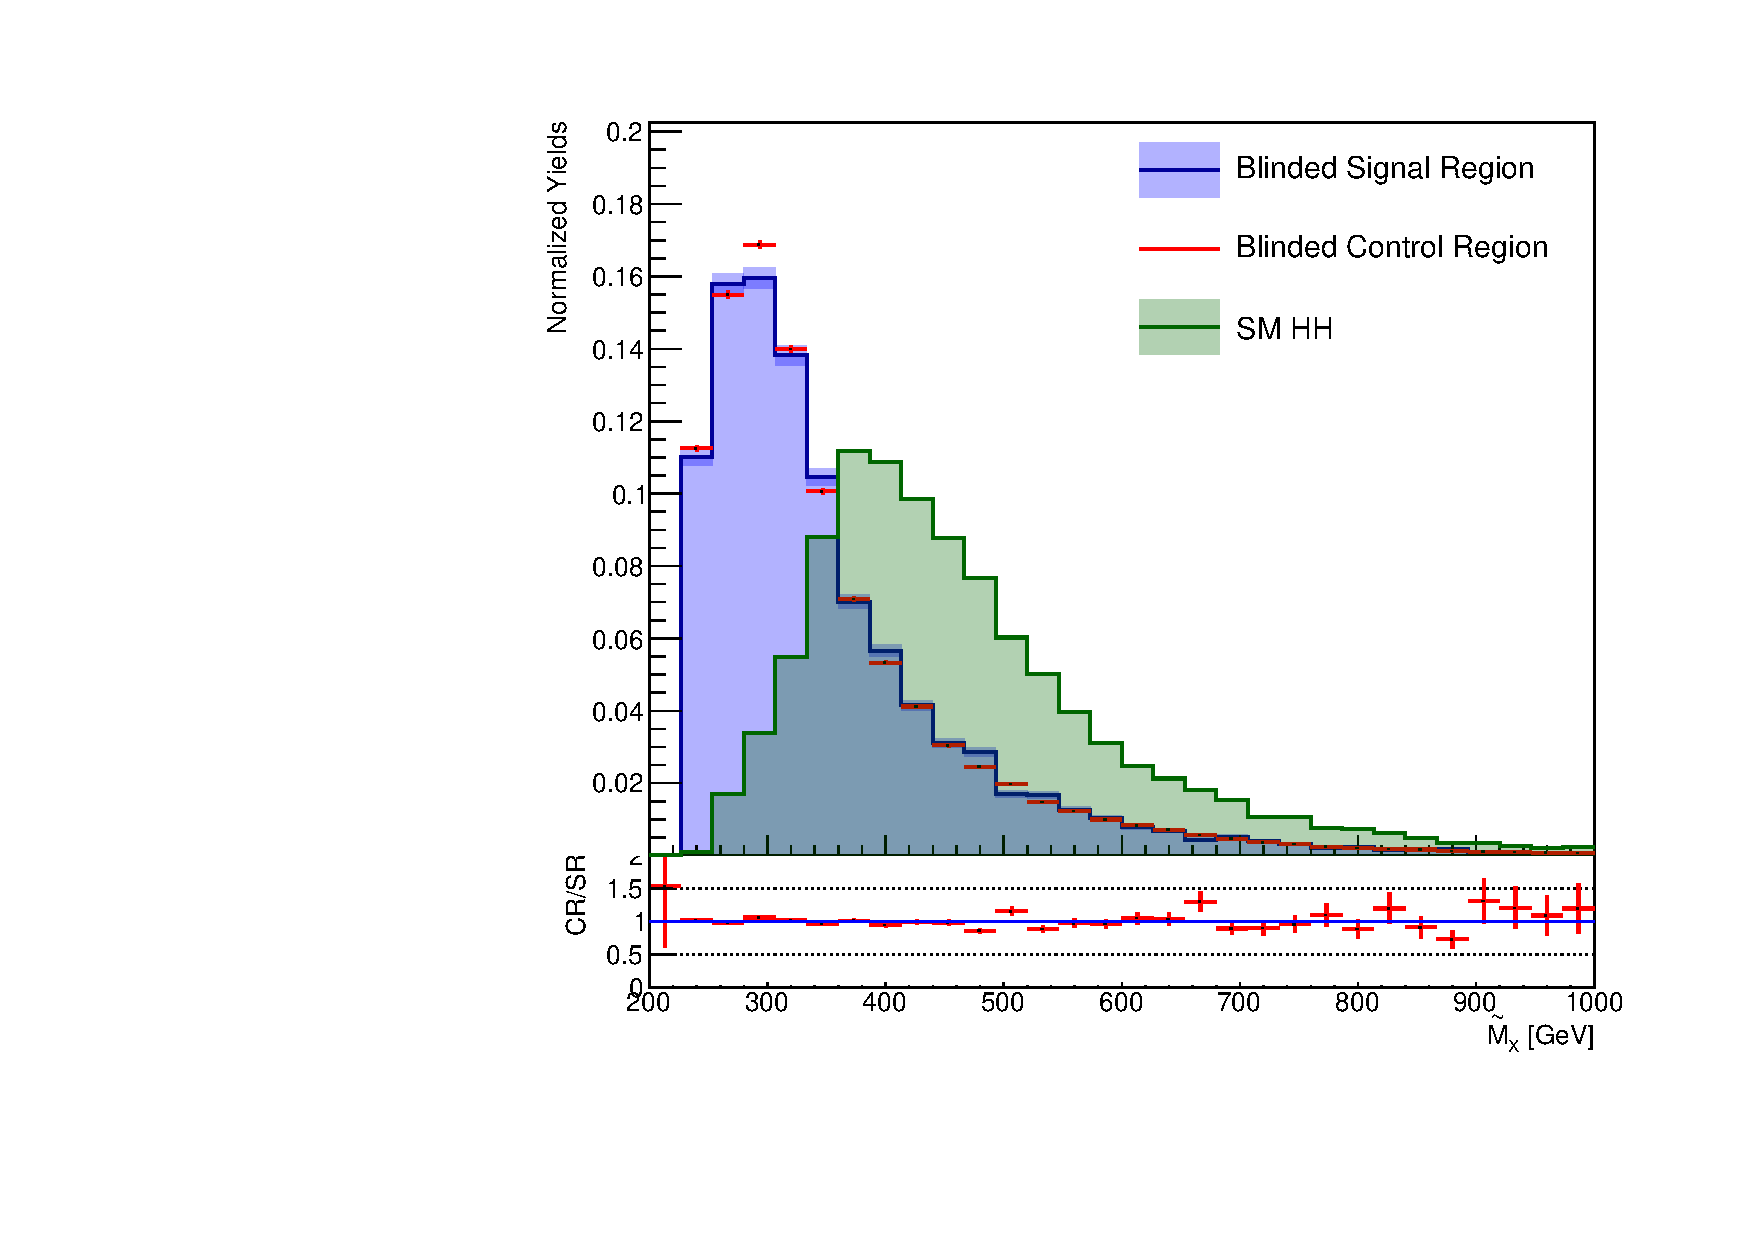
\includegraphics[width=0.45\textwidth]{figures/sec-cats/mx}\hfil
  \caption{Comparison between blinded signal region and blinded photon control region in the leading jet b-tagging, subleading jet b-tagging and effective mass.}
  \label{fig:PCR_plots}
\end{figure*}

By checking the ratio between the distributions of the signal region and the photon control region, before normalization, it was found that the photon control region 
needs to be scaled by a factor of $0.14$ in order to also be consistent in terms of yields with the signal region. 
By the time this optimization was performed, only 22/fb of prompt reco data was available, therefore, the control region was also scaled by a factor of $35/22$ in order to match 
the expected full integrated luminosity of 2016. 
For the significance calculation, we assume the SM HH signal with a cross section of 1 fb and an integrated luminosity of 35/fb. 
We then calculate the significance of each exclusive b-tagging bin in the b-tagging 2D plane, as shown in Figure \ref{fig:2D_sig_btag}. 

\begin{figure*}[thb]
  \centering
  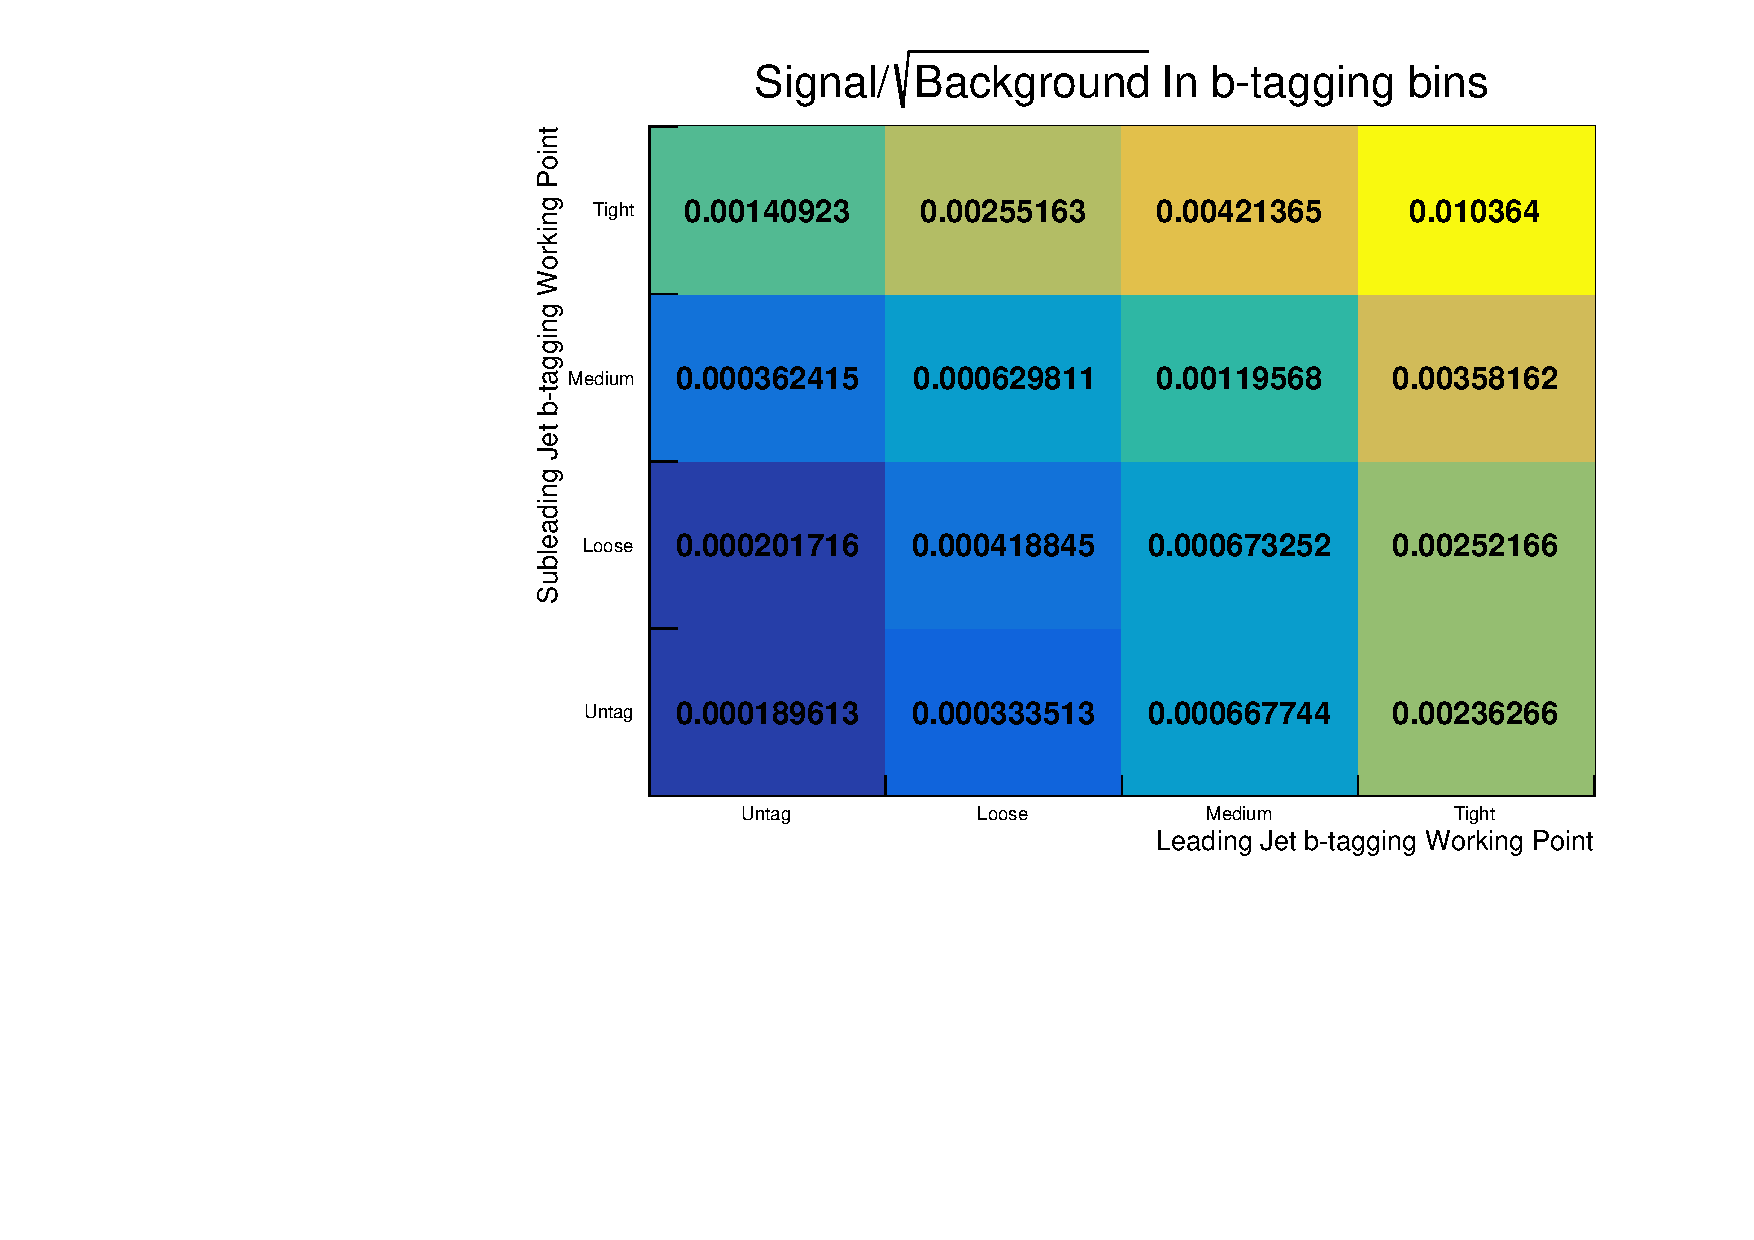
\includegraphics[width=0.45\textwidth]{figures/sec-cats/2DbtagSig}\hfil
  \caption{Sigificance in exclusive b-tagging bins in the 2D plane defined by the b-tagging score of the selected leading and subleading jet candidates.}
  \label{fig:2D_sig_btag}
\end{figure*}

With that in mind, we construct different options for the categorization schemes. These can be seen in Figure \ref{fig:differentcats}. 
The green squares represent the High Purity Category (HPC), the yellow squares represent the Medium Purity Category (MPC) and the blue squares represent 
the Jet Control Region (JCR). 

\begin{figure*}[thb]
  \centering
  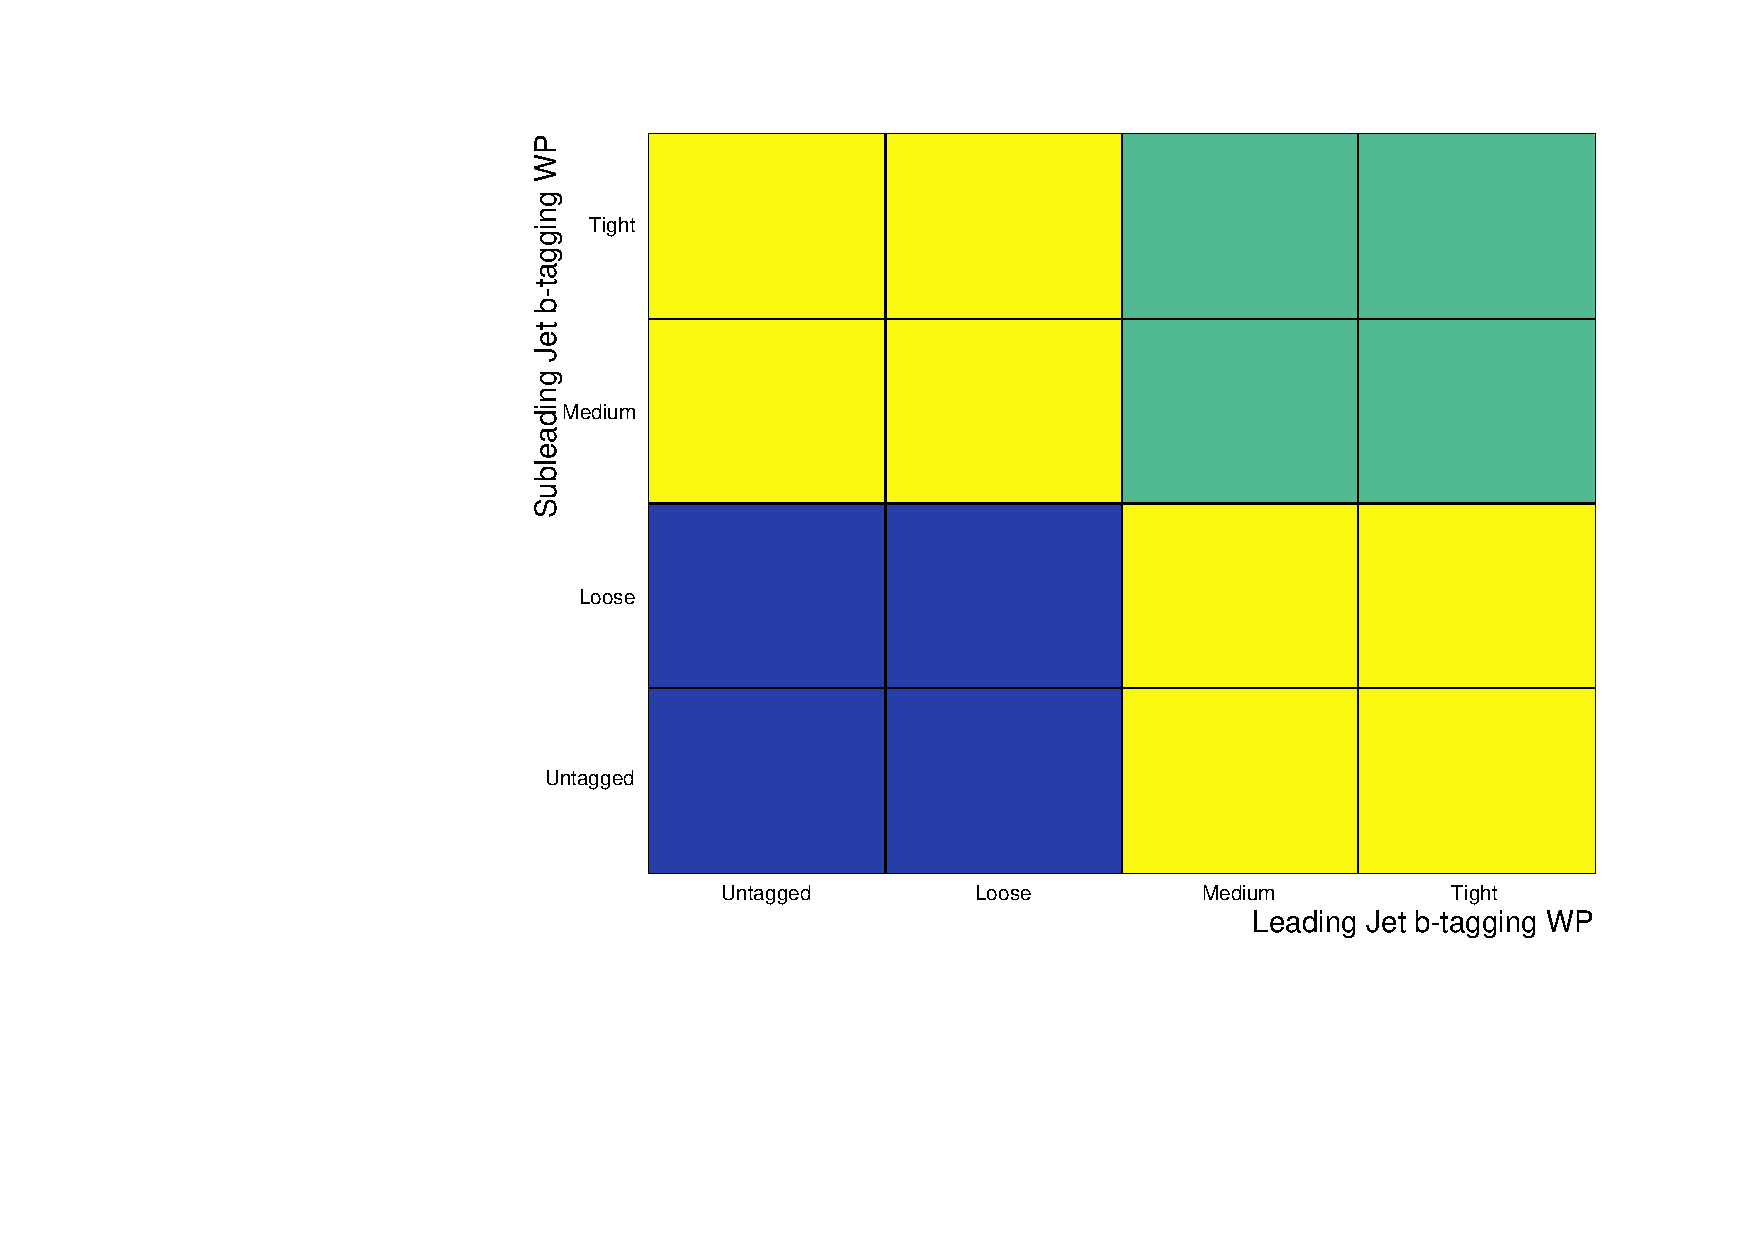
\includegraphics[width=0.25\textwidth]{figures/sec-cats/catPlot_Run1}\hfil
  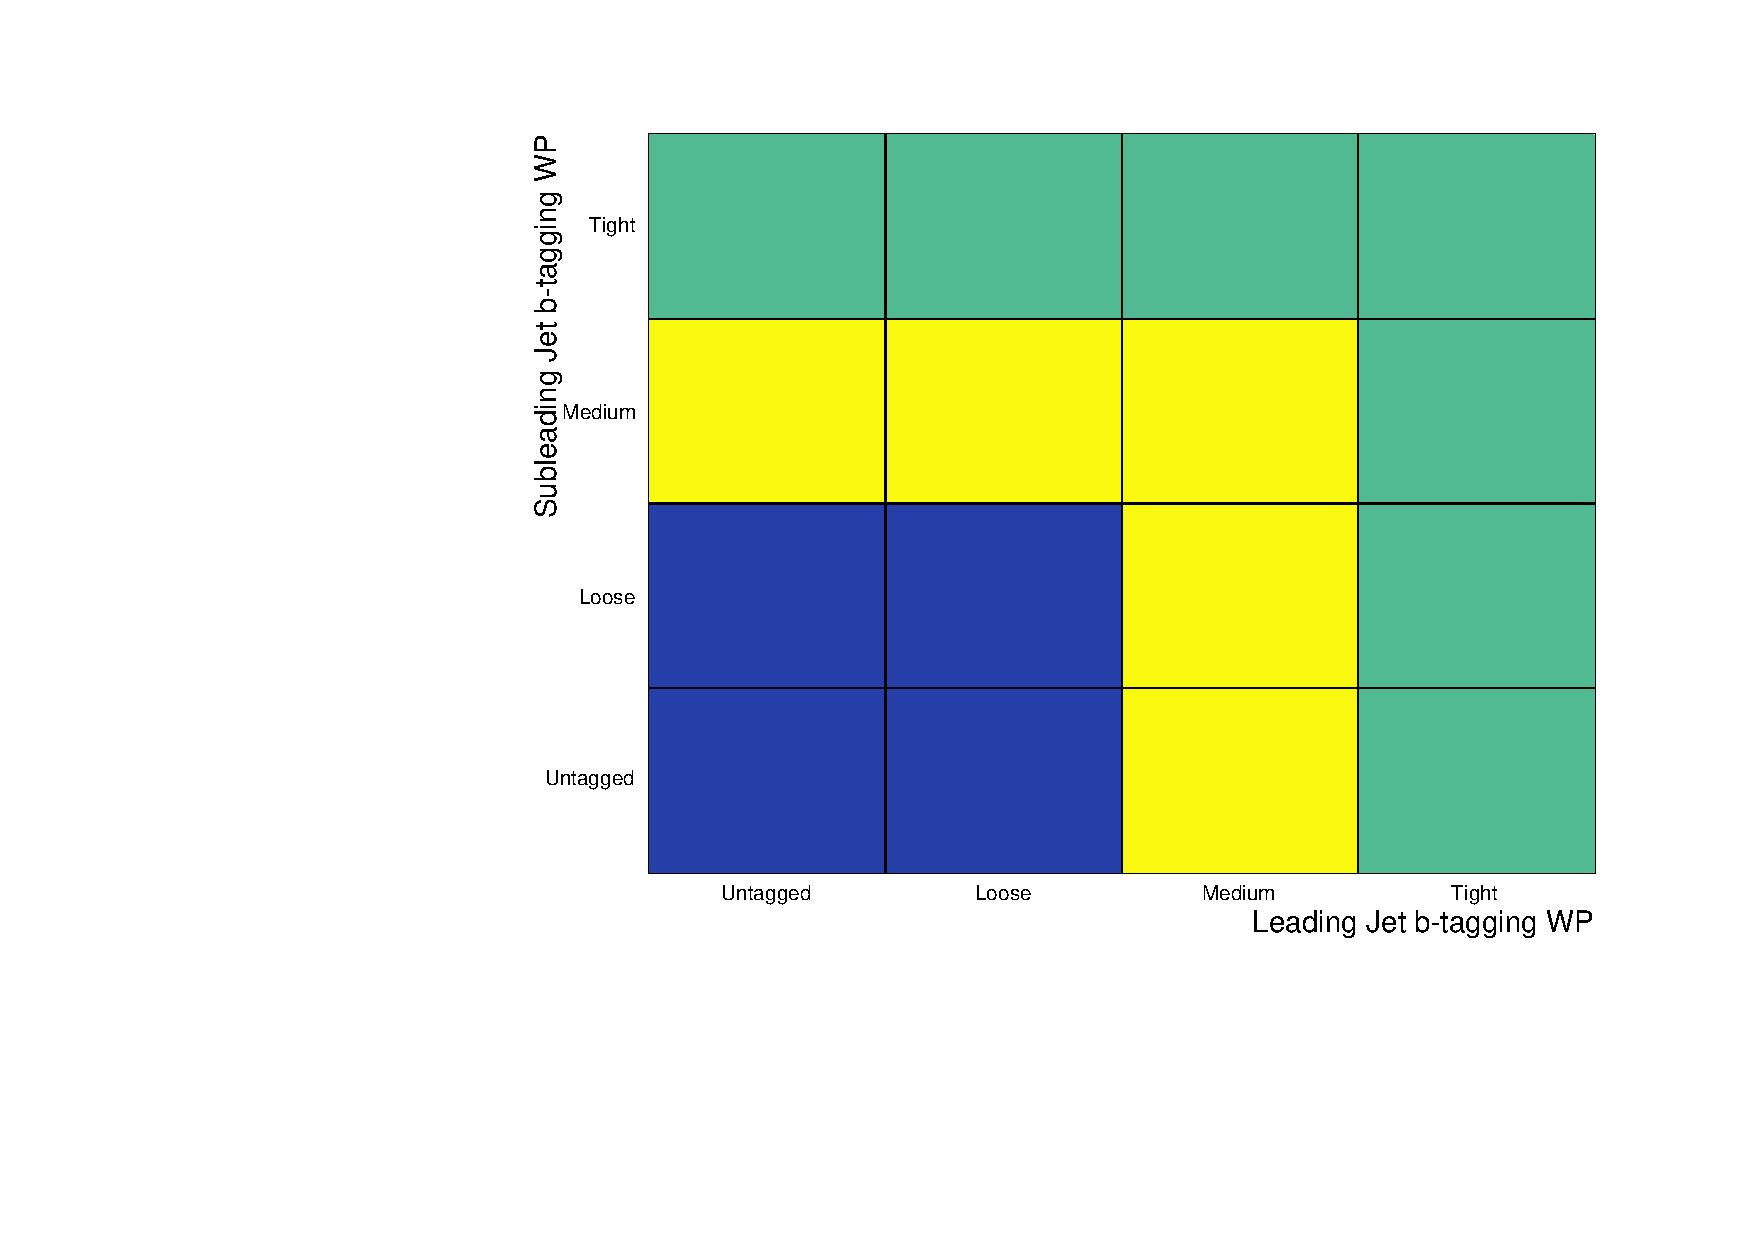
\includegraphics[width=0.25\textwidth]{figures/sec-cats/catPlot_2015}\hfil
  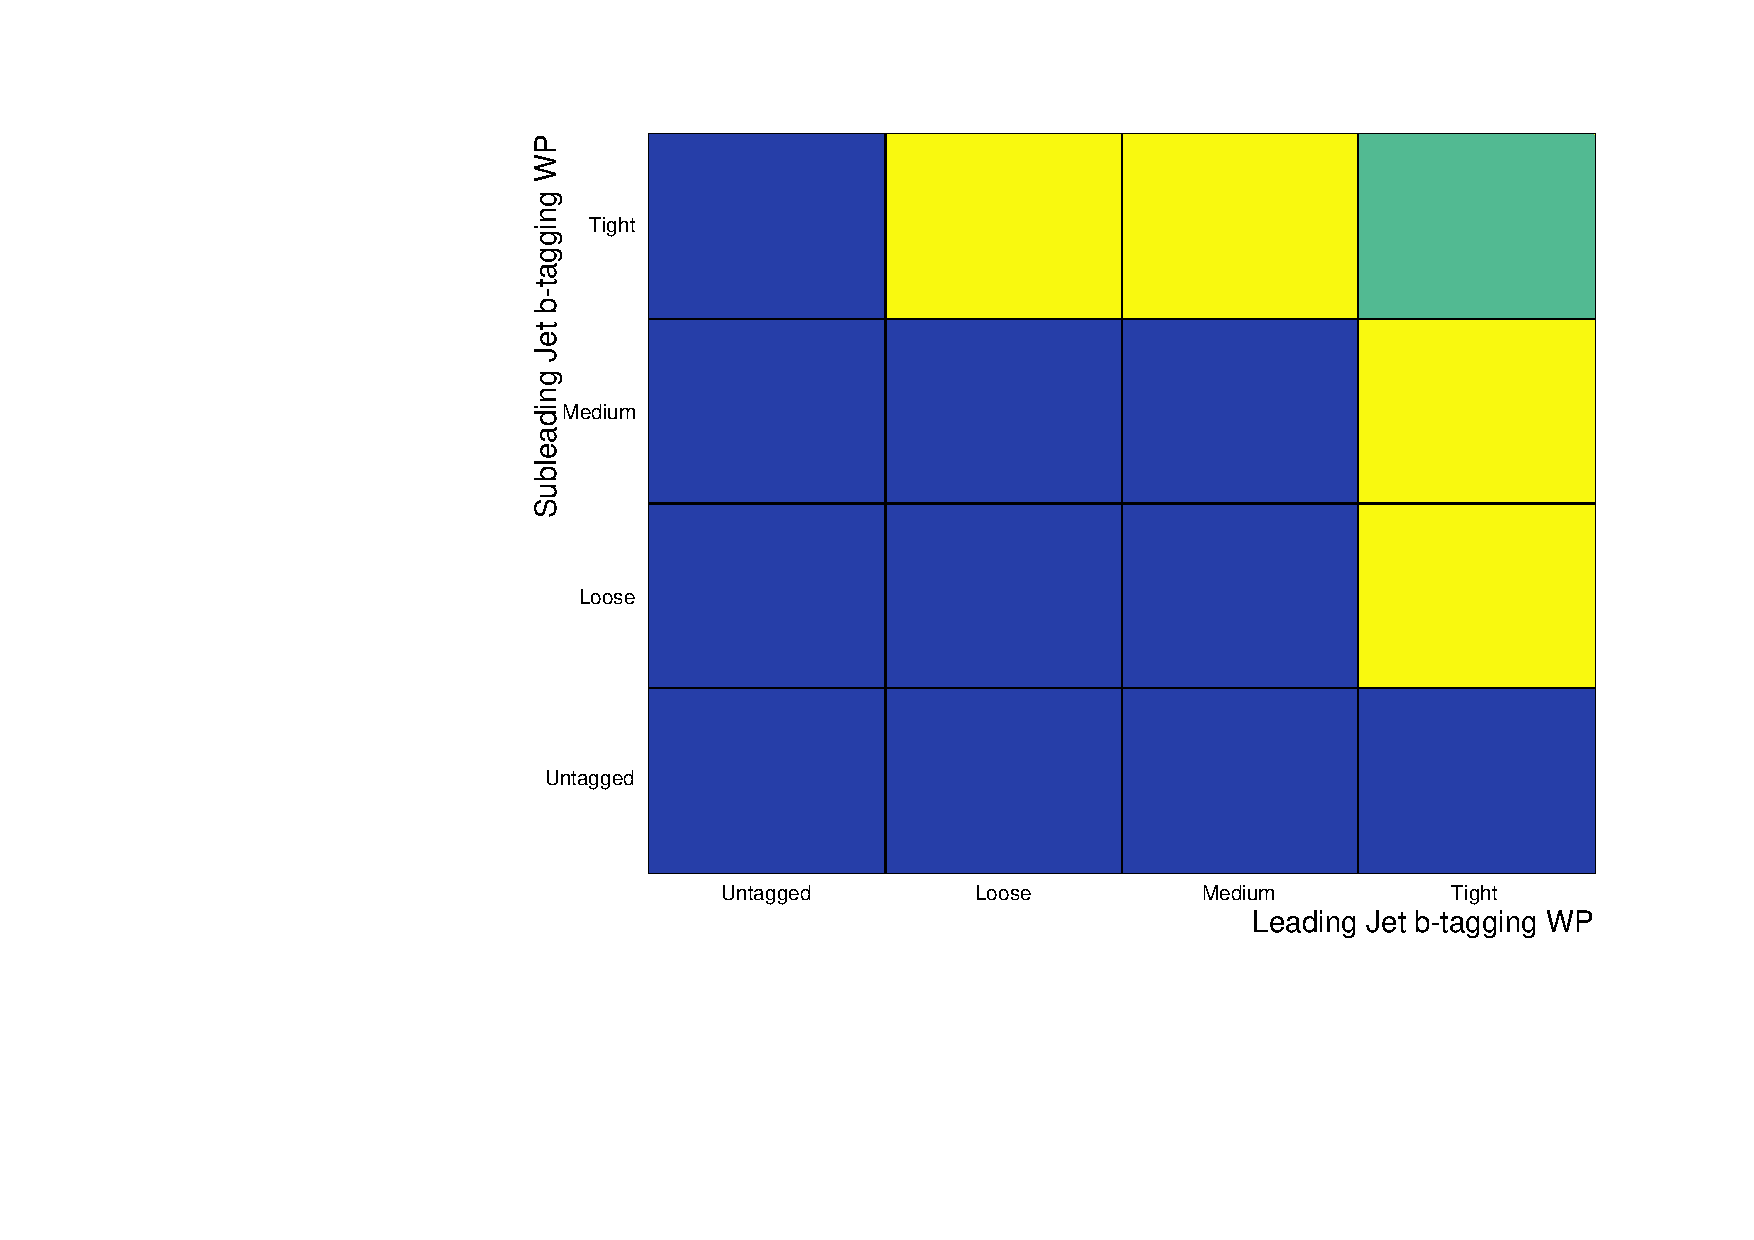
\includegraphics[width=0.25\textwidth]{figures/sec-cats/catPlot_NonRes}\hfil
  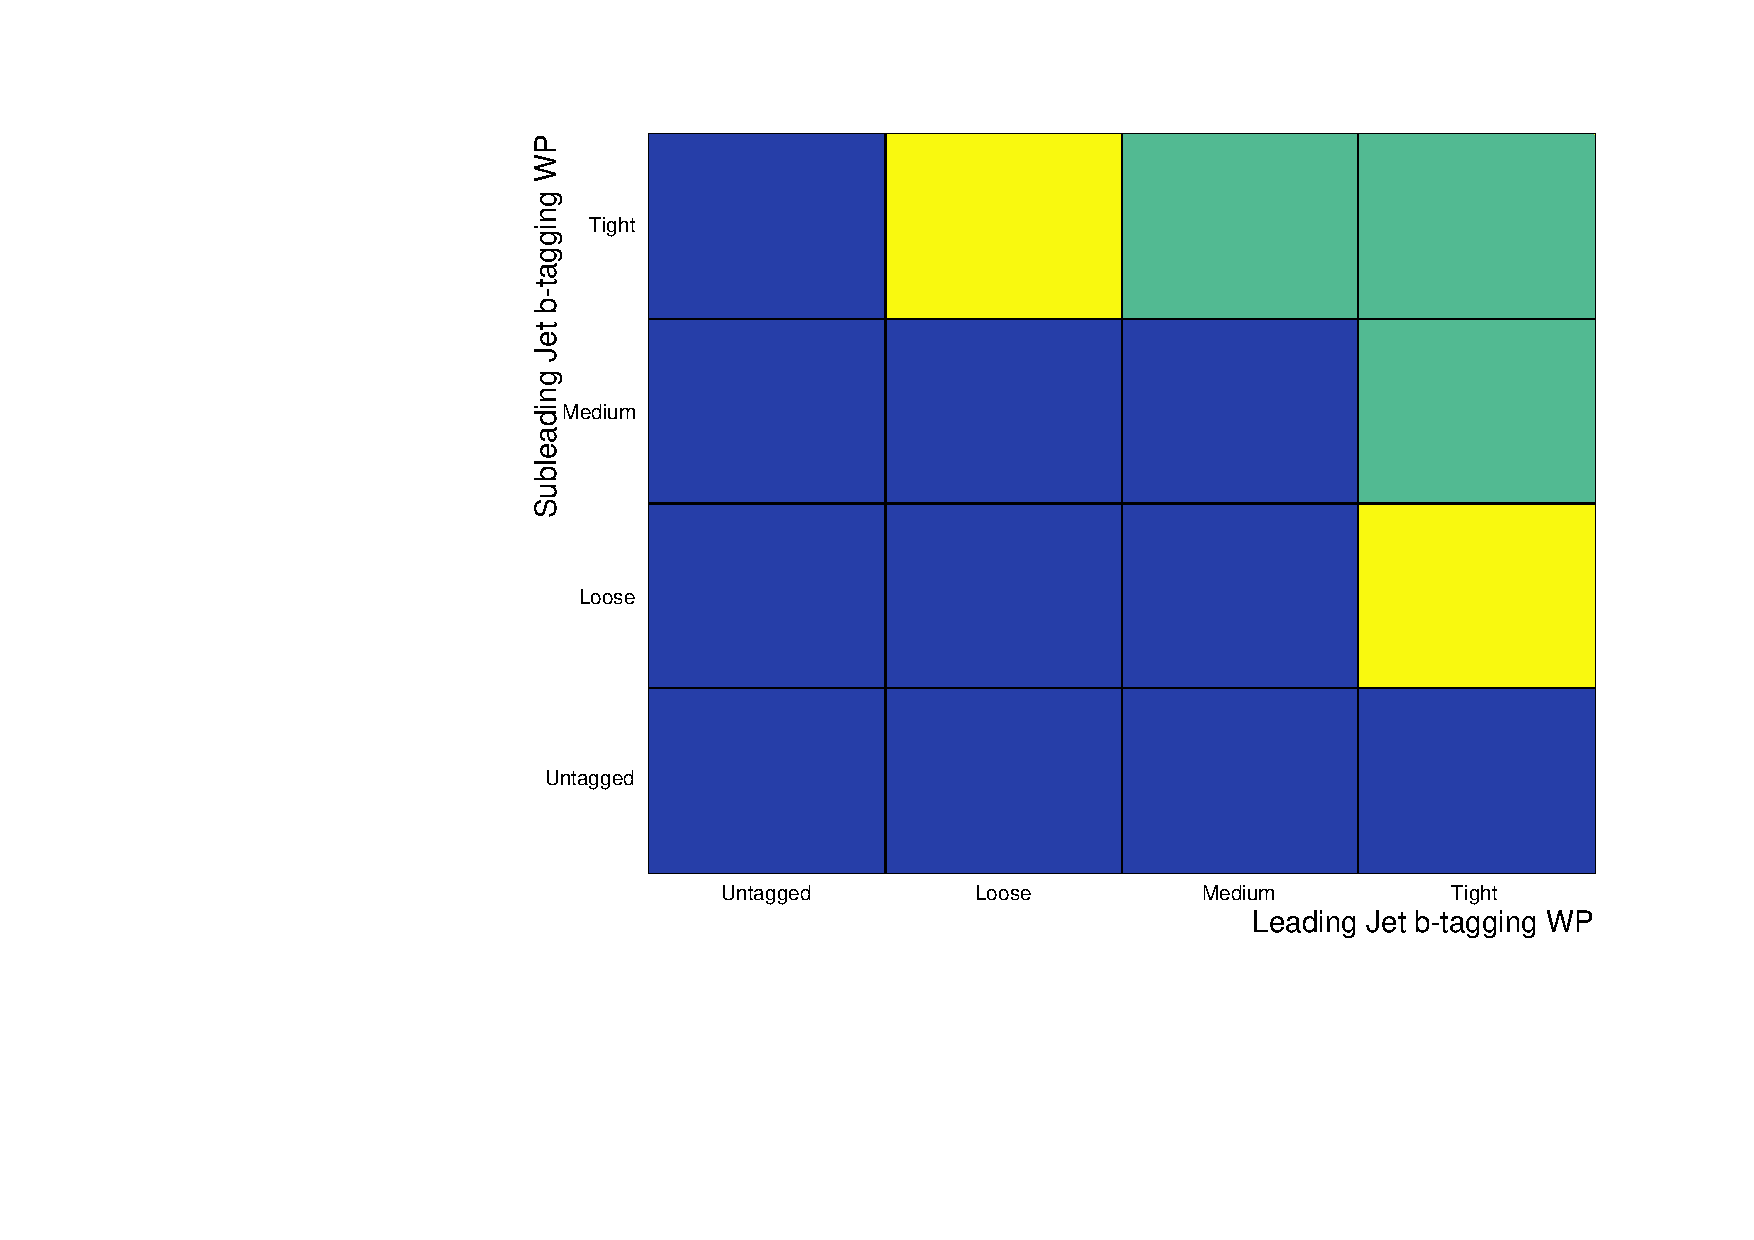
\includegraphics[width=0.25\textwidth]{figures/sec-cats/catPlot_DEF2}\hfil
  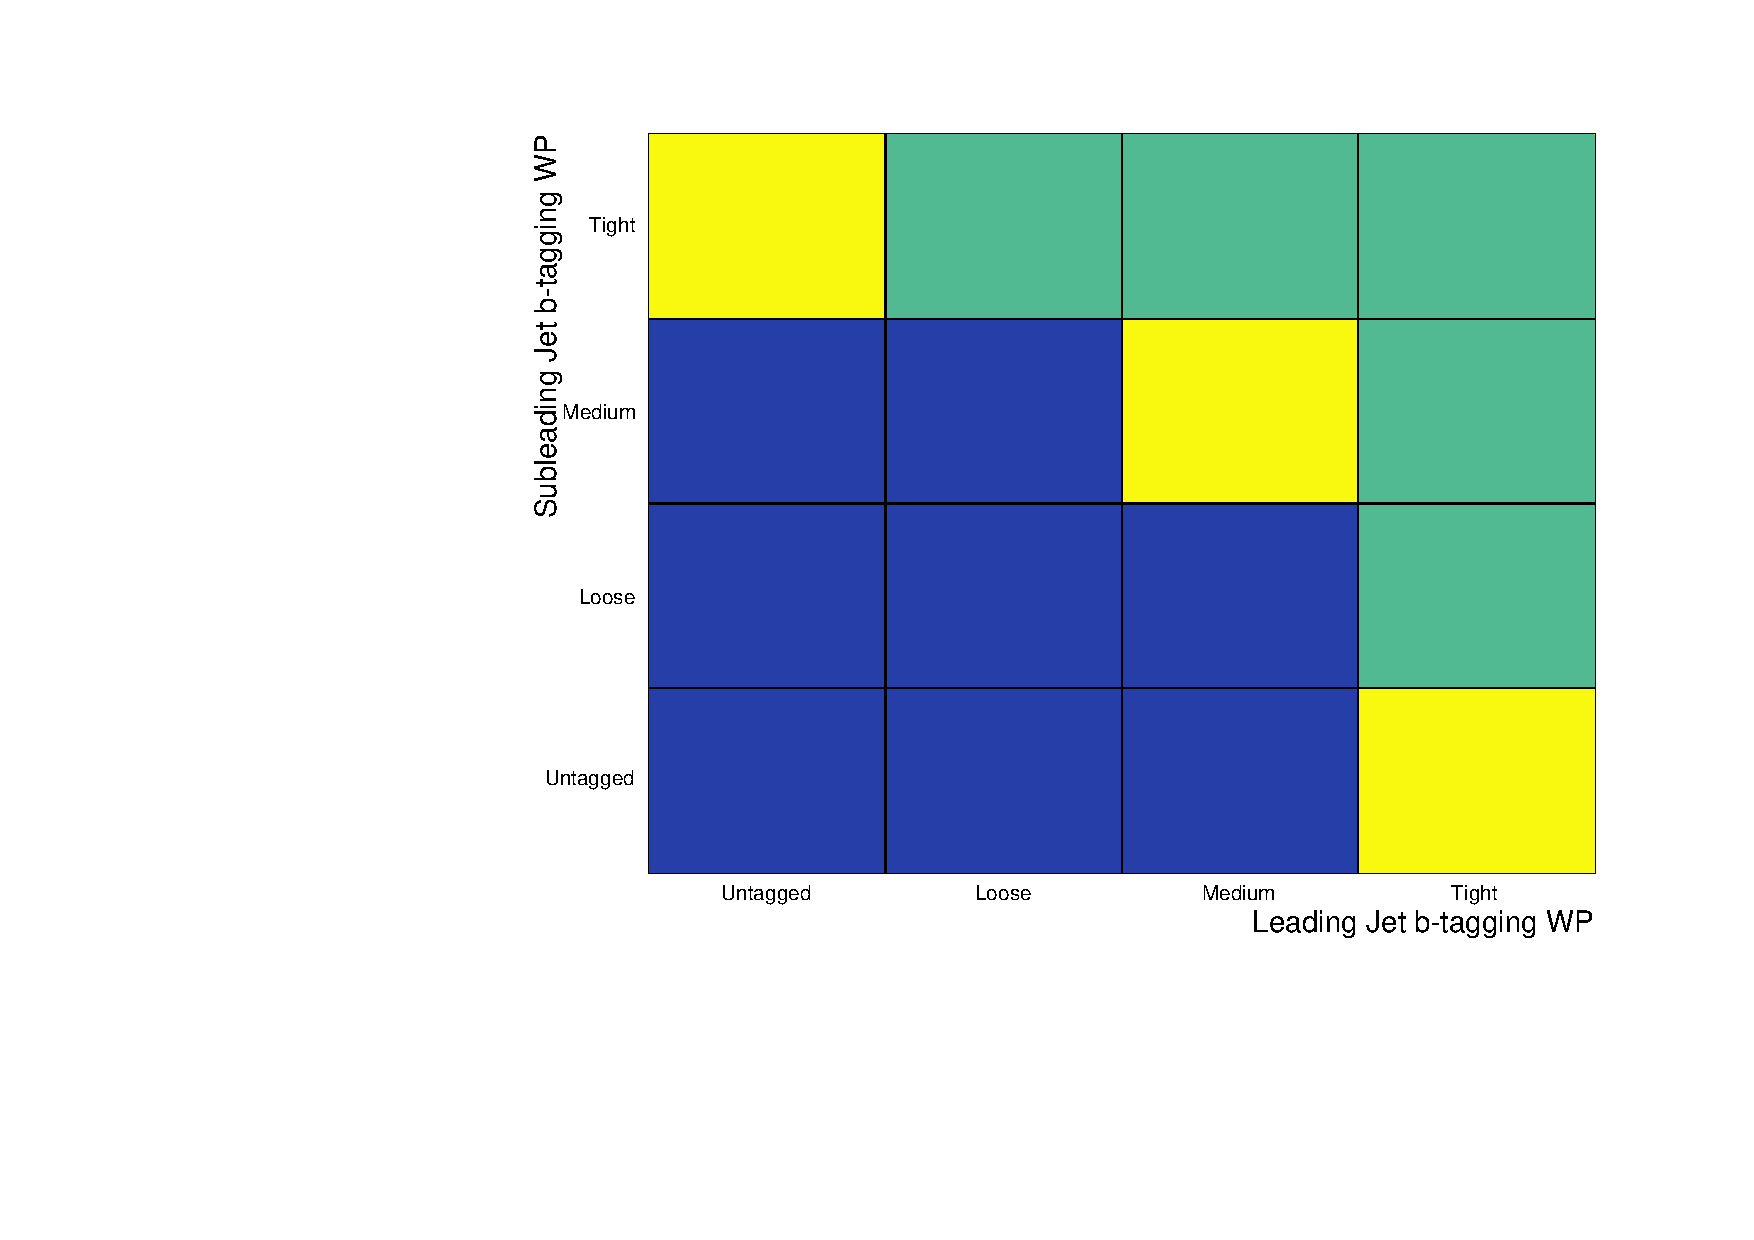
\includegraphics[width=0.25\textwidth]{figures/sec-cats/catPlot_DEF3}\hfil
  \caption{Different categorization strategies, from left to right, Run 1 categorization, 2015 low mass resonant categorization, Non-resonant option, Option 2 and Option 3.}
  \label{fig:differentcats}
\end{figure*}

Another point that needs to be checked during the categorization is the expected number of background events. 
Since our background estimation is data driven, with the sidebands of the diphoton and dijet mass distributions, we need to make sure some events are left to fit. 
Therefore, we apply the mass window requirement (for the resonant case) and the $\tilde{M}_{X}$ categorization (for the non-resonant case) and check the amount of expected background events. 
For the non-resonant case, we found that even using the most strict categorization definitions, we would still have enough expected background events for a robust description. 
For the resonant case, we test the different categorization schemes showin in Figure \ref{fig:differentcats} to see the expected number of background events (with the photon control region) on both HPC and MPC. 
These mass scans can be seen in Figure \ref{fig:expbackground}. 

\begin{figure*}[thb]
  \centering
  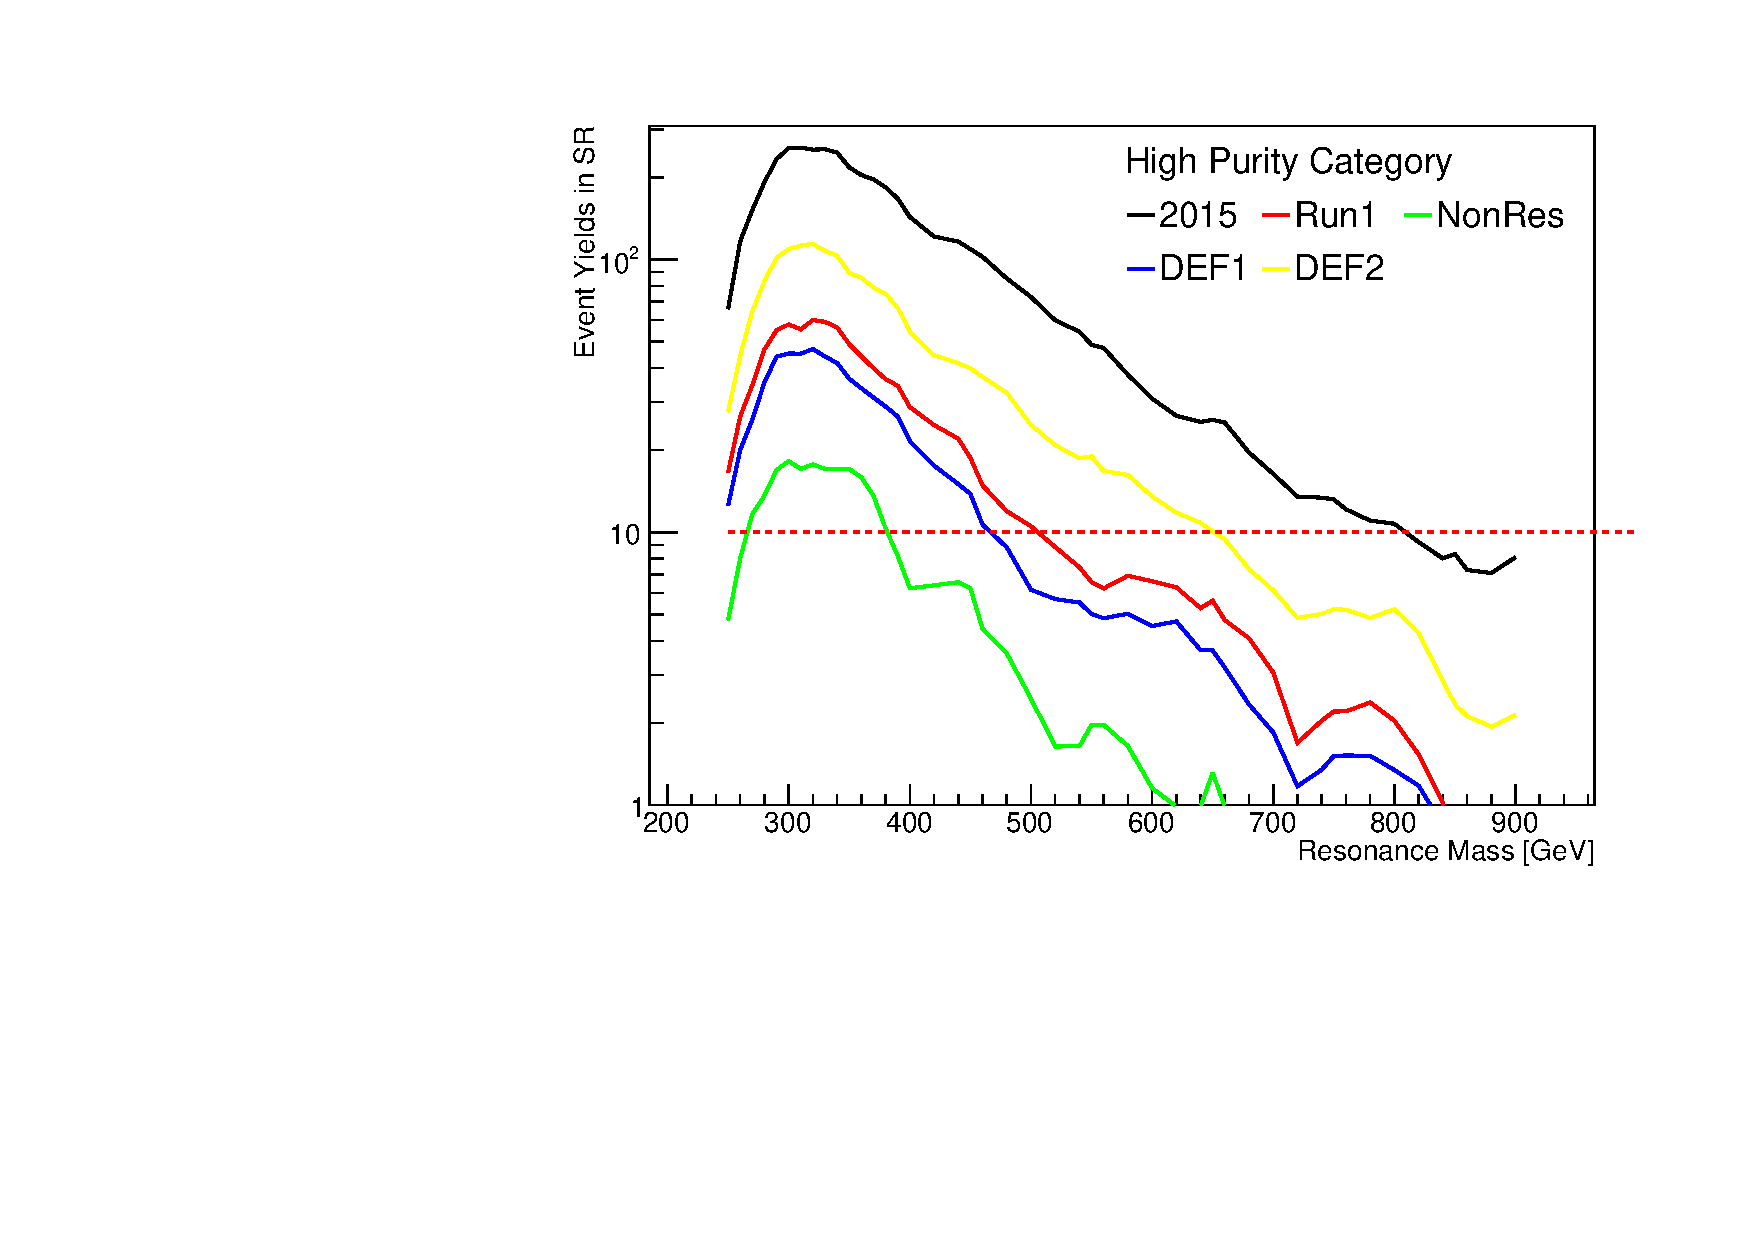
\includegraphics[width=0.45\textwidth]{figures/sec-cats/yields_cat0}\hfil
  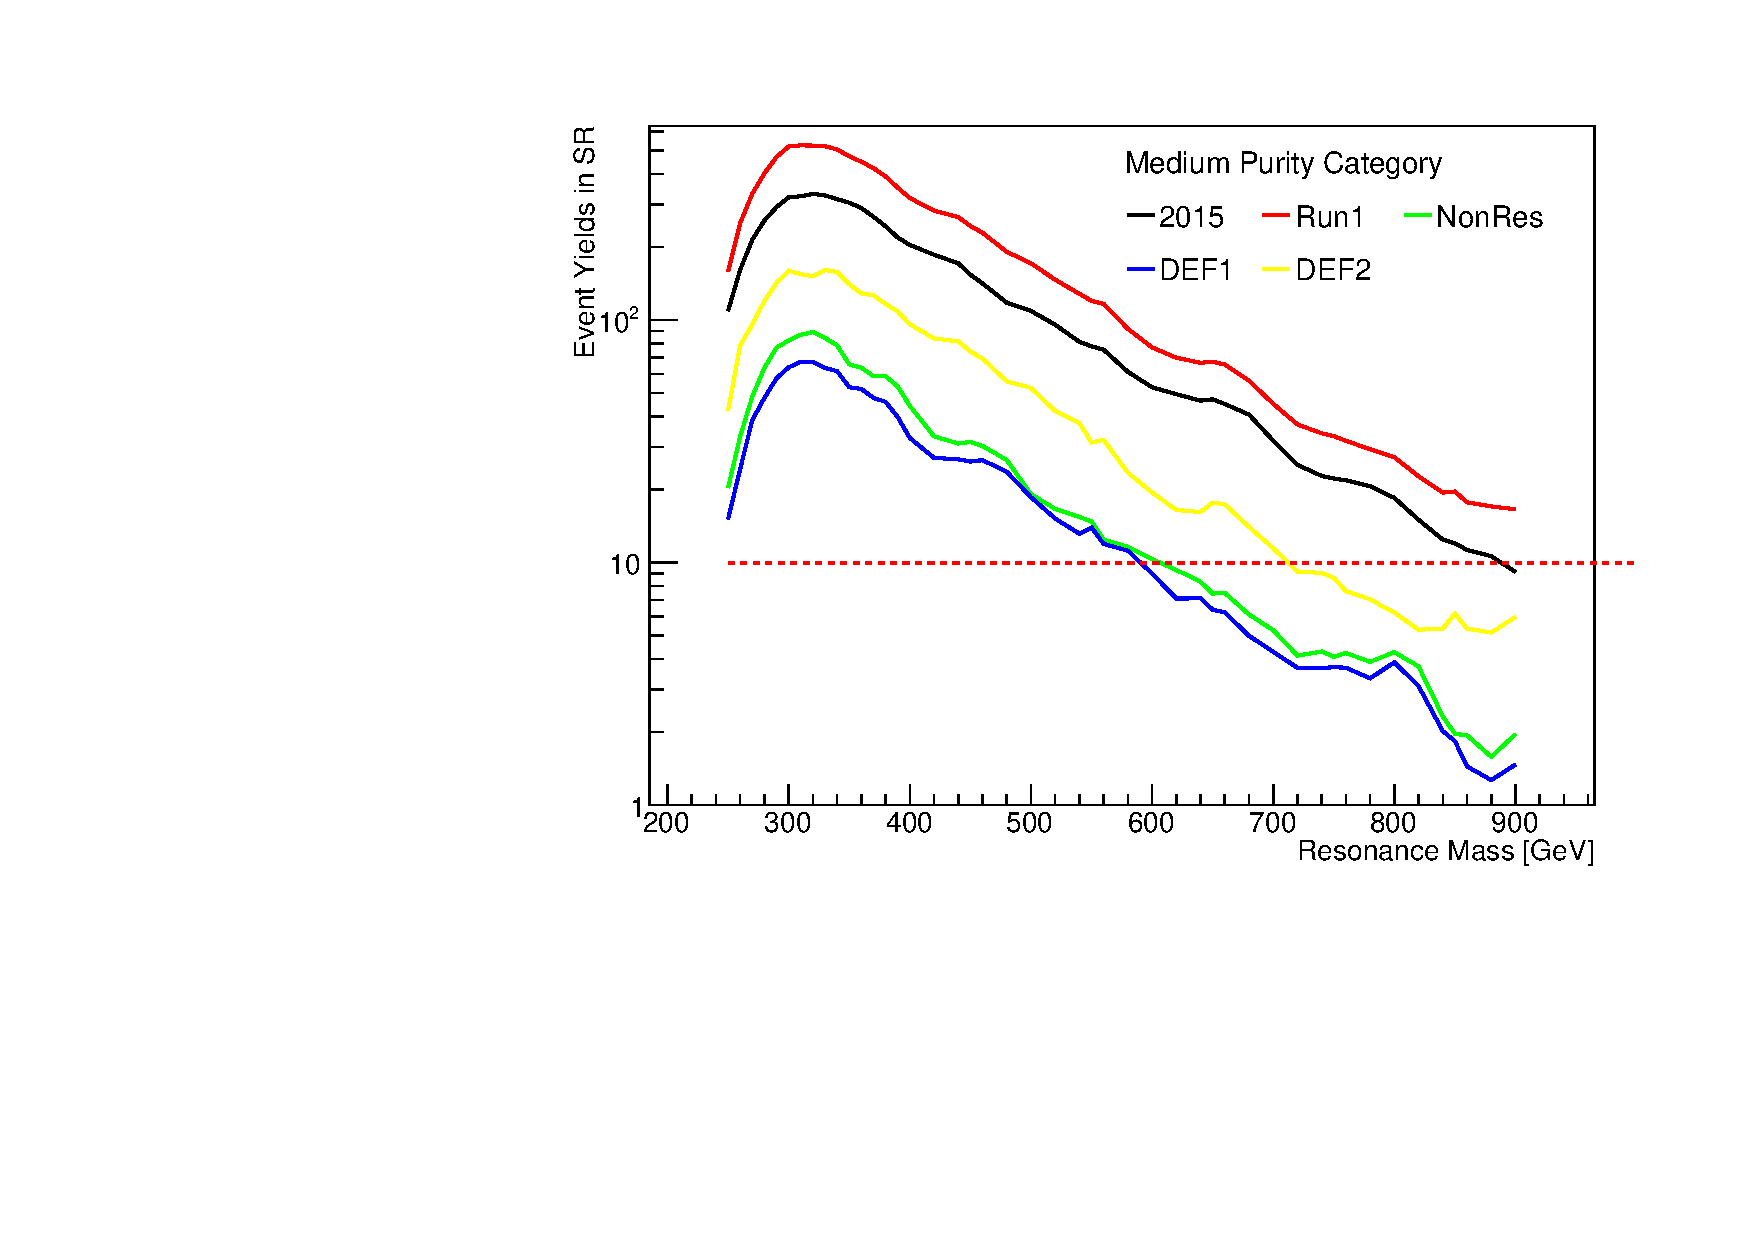
\includegraphics[width=0.45\textwidth]{figures/sec-cats/yields_cat1}\hfil
  \caption{Expected background yields, from the photon control region scaled to the signal region, for the different resonant mass points (including mass window requirement), for the HPC and the MPC, respectively. 
Please note that "DEF1" in the legend corresponds to Option $2$ in the diagrams of Figure \ref{fig:differentcats}, while "DEF2" corresponds to Option 3. }
  \label{fig:expbackground}
\end{figure*}

From Figure \ref{fig:expbackground}, we see that the non-resonant proposed categorization is too tight for most of the resonance masses in both categories. 
Option 2 seems to give a reasonable amount of background events for the modeling up until the boundary used in 2015 to define the low/high resonant regions. 
Therefore, for the low mass resonant analysis ($\tilde{M}_{X} < 500 $ GeV), we use the categorization under Option 2 in the diagrams of Figure \ref{fig:differentcats}. 
For the High mass resonant analysis ($\tilde{M}_{X} > 500 $ GeV), we use the same categorization scheme that was used for the 2015 low mass resonant analysis. 

In addition to the categories mentioned above, cuts on the helicity angle $|cos(\theta^{*}_{CS})|$ have been investigated. 
It was found that the cut that maximizes the sensitivity of the analysis is at 0.80 for the non-resonant categories. 
No cut is imposed in the resonant analysis. 

\subsection{MVA Categorization}

During the analysis, it has been noticed that different kinematic variables could potentially contribute to tightening the signal region without cutting too much on the signal efficiency. 
However, this large-dimensional optimization procedure (all investigated variables) was not optimal. 
Instead, we have developed a multivariate analysis (MVA), combining these different variables, into a single discriminant. 
This discriminant is used to categorize the events in High Purity, Medium Purity categories and a control region, similarly to the cut based categorization. 

The input variables investigated for this MVA were:
\begin{itemize}
\item Leading and subleading jets b-tagging score;
\item Helicity angles $|cos(\theta^{*}_{CS})|$, $|cos(\theta^{*}_{bb})|$ and $|cos(\theta^{*}_{\gamma\gamma})|$: $|cos(\theta^{*}_{CS})|$ is defined as the angle between the direction of the $H\rightarrow\gamma\gamma$ candidate to the Colin-Sopper reference frame (assumes each incoming particle in the scattering to have 6.5 TeV); $|cos(\theta^{*}_{xx})|$ is defined as the angle between the particle $x$ and the direction defined by the $H\rightarrow x x$ candidate (randomly choosing between x's), where $x = \gamma$ or $b$;
\item $p_{T}(\gamma\gamma)/M(jj\gamma\gamma)$ and $p_{T}(jj)/M(jj\gamma\gamma)$
\end{itemize}

The training was performed in the photon control region, as described in \ref{sec:PCR}, modeling our background. 
Plots comparing the input variables in the photon control region and the blinded signal region are shown in Figure \ref{fig:inputmva}. 
As our signal in the training, we sum the 14 non-resonant HH samples available (box only, SM, and 12 BSM points). 
Thus, we have a training that is not specific to a single region in the parameter space, maintaining the sensitivities comparable between the benchmark points (as it is with the cut based categorization). 

\begin{figure*}[thb]
  \centering
  \includegraphics[width=0.3\textwidth]{figures/sec-cats/mva/ljbdis}\hfil
  \includegraphics[width=0.3\textwidth]{figures/sec-cats/mva/sjbdis}\hfil
  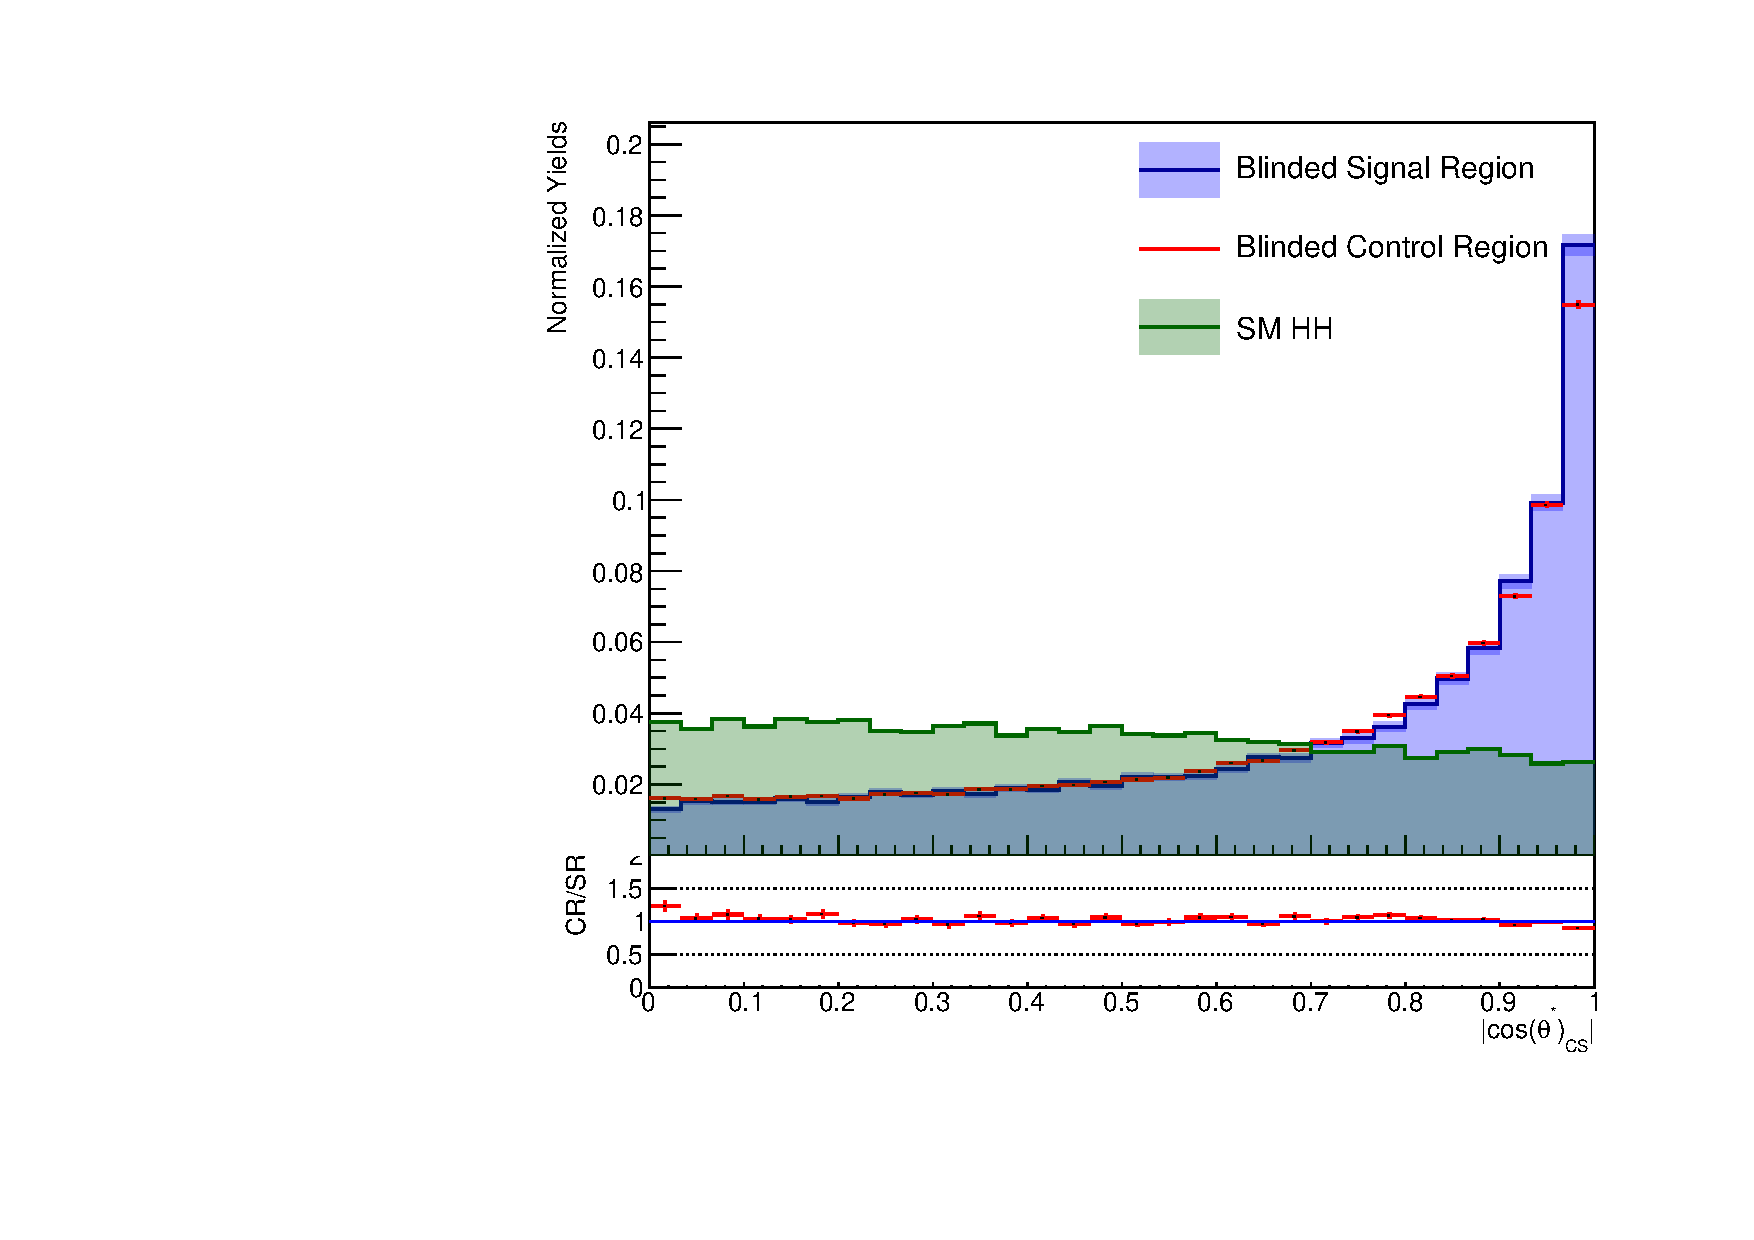
\includegraphics[width=0.3\textwidth]{figures/sec-cats/mva/cts_cs}\hfil
  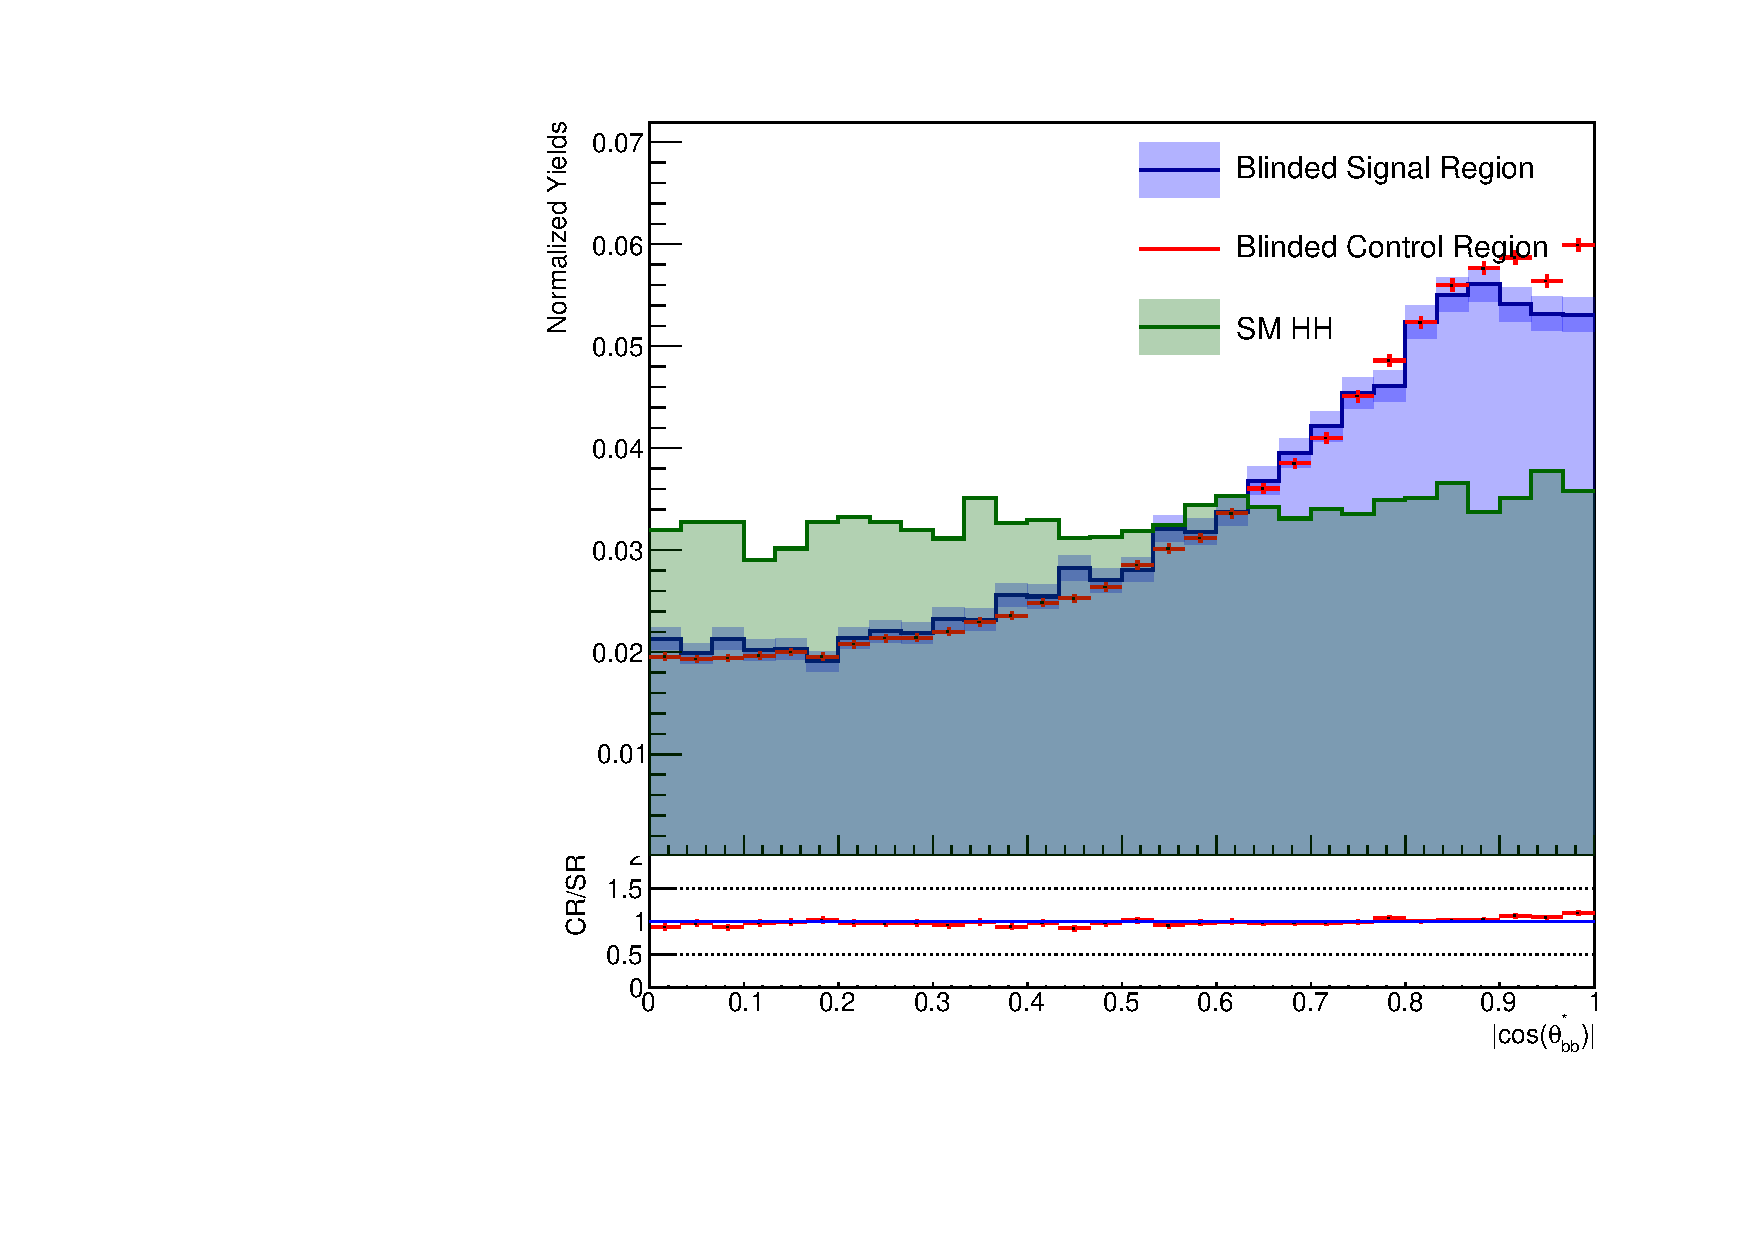
\includegraphics[width=0.3\textwidth]{figures/sec-cats/mva/ct_bb}\hfil
  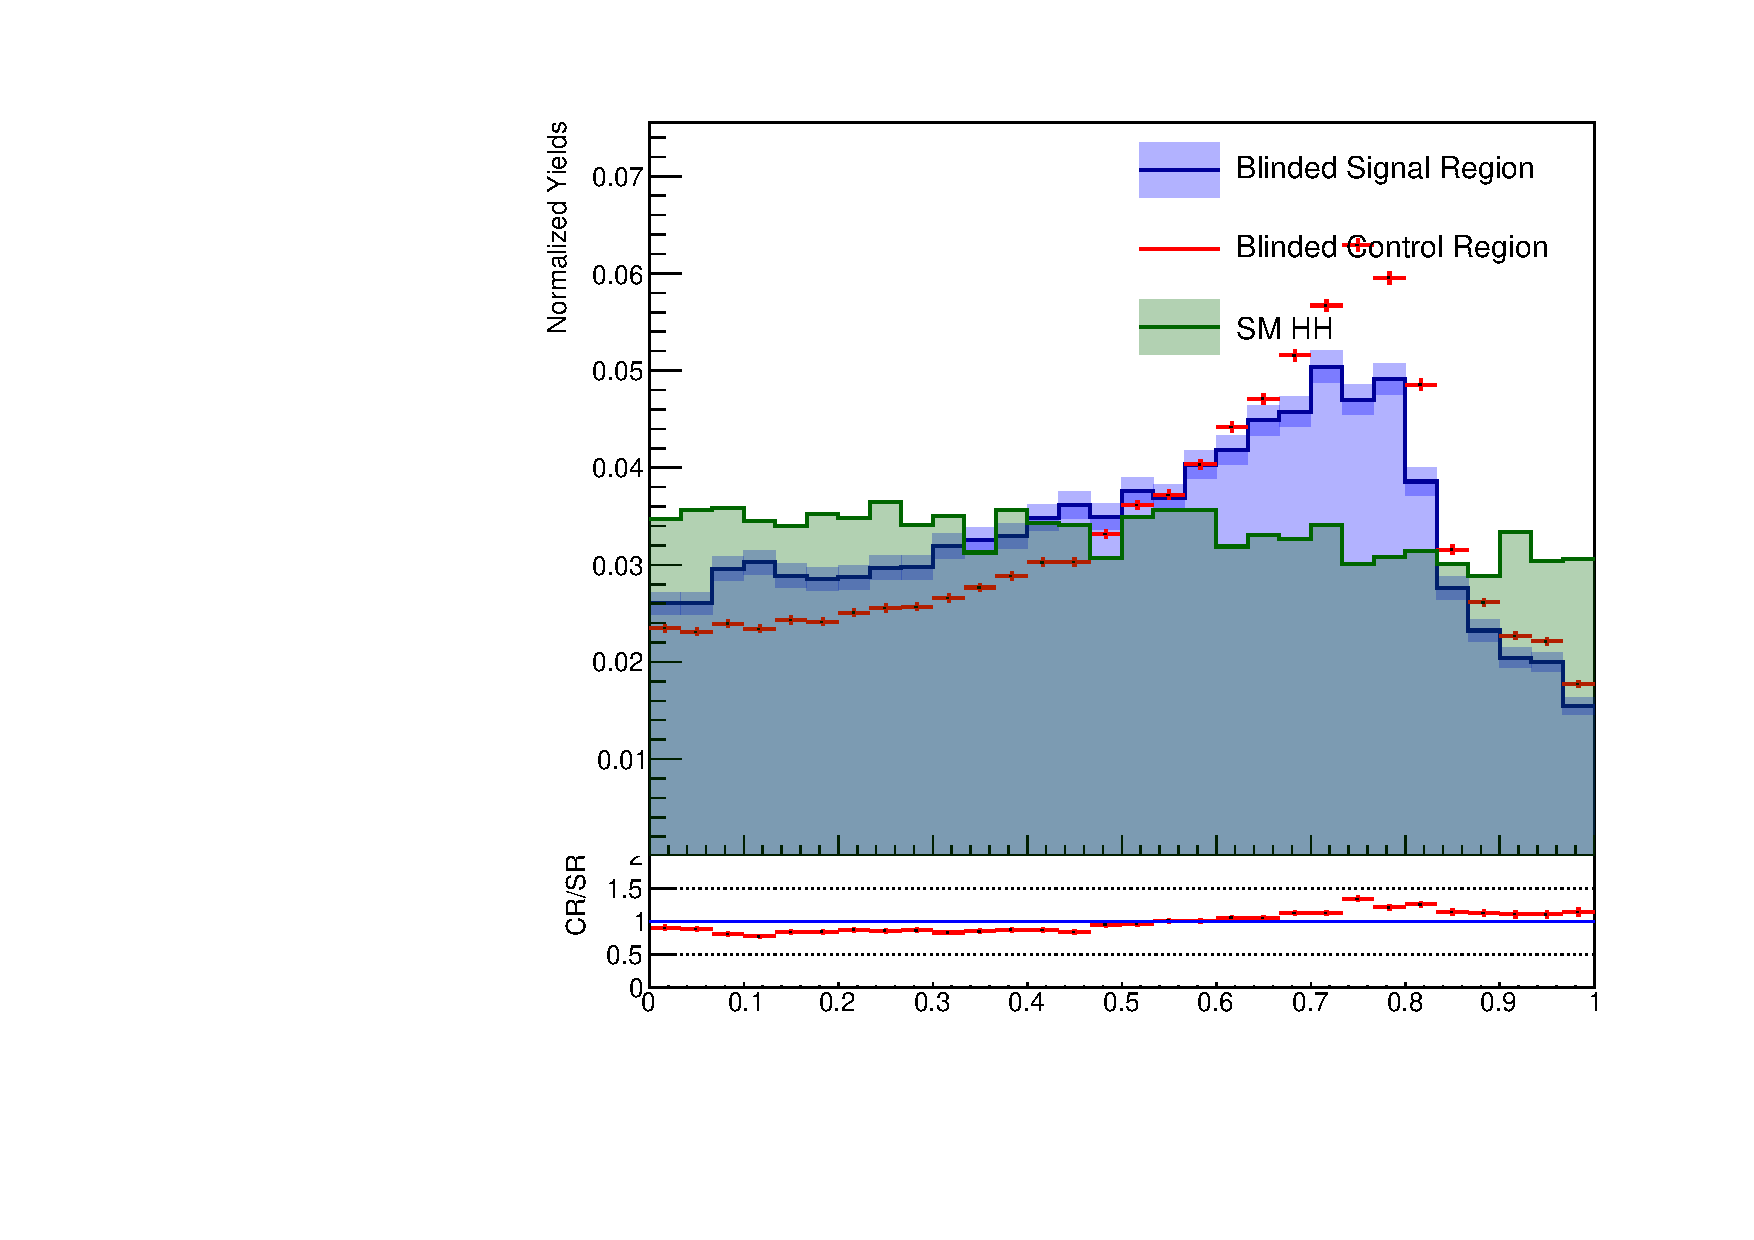
\includegraphics[width=0.3\textwidth]{figures/sec-cats/mva/ct_gg}\hfil
  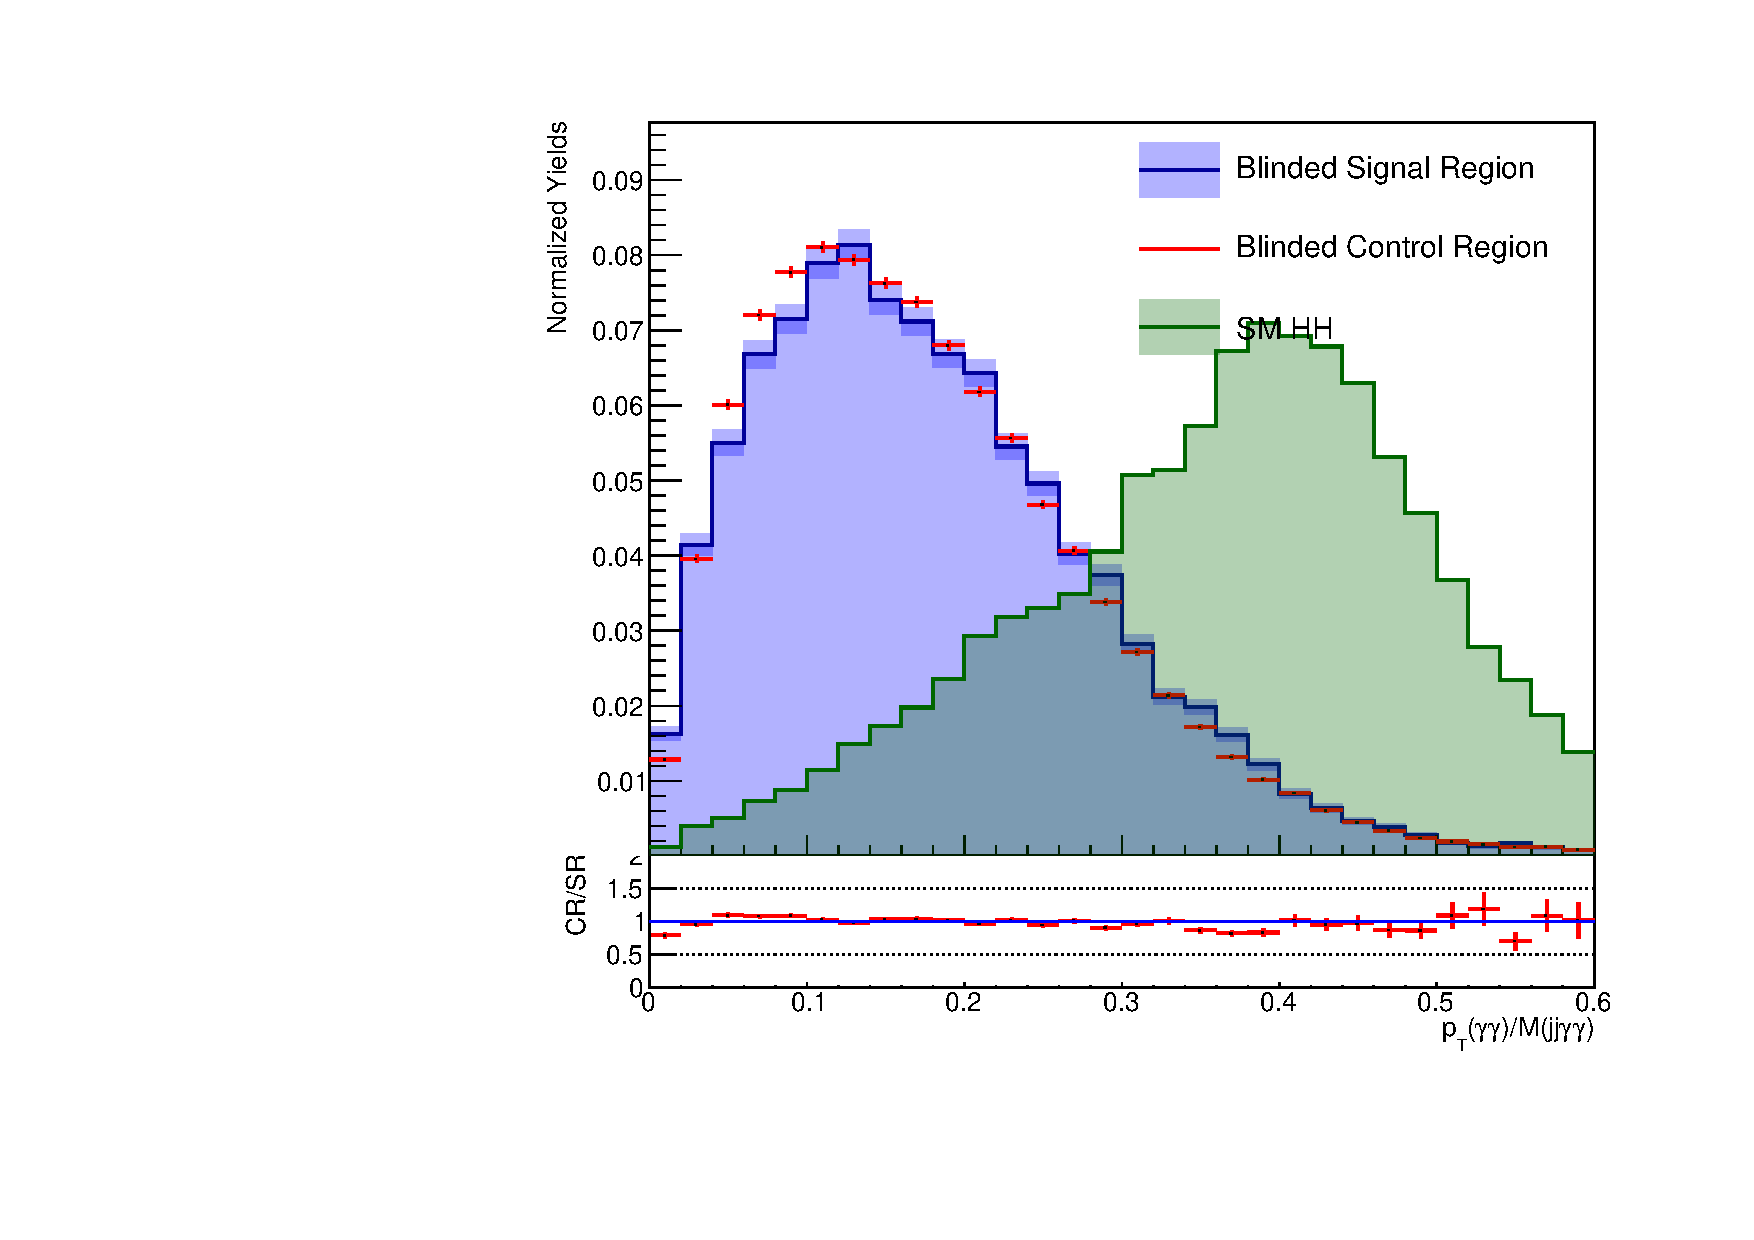
\includegraphics[width=0.3\textwidth]{figures/sec-cats/mva/gghhr}\hfil
  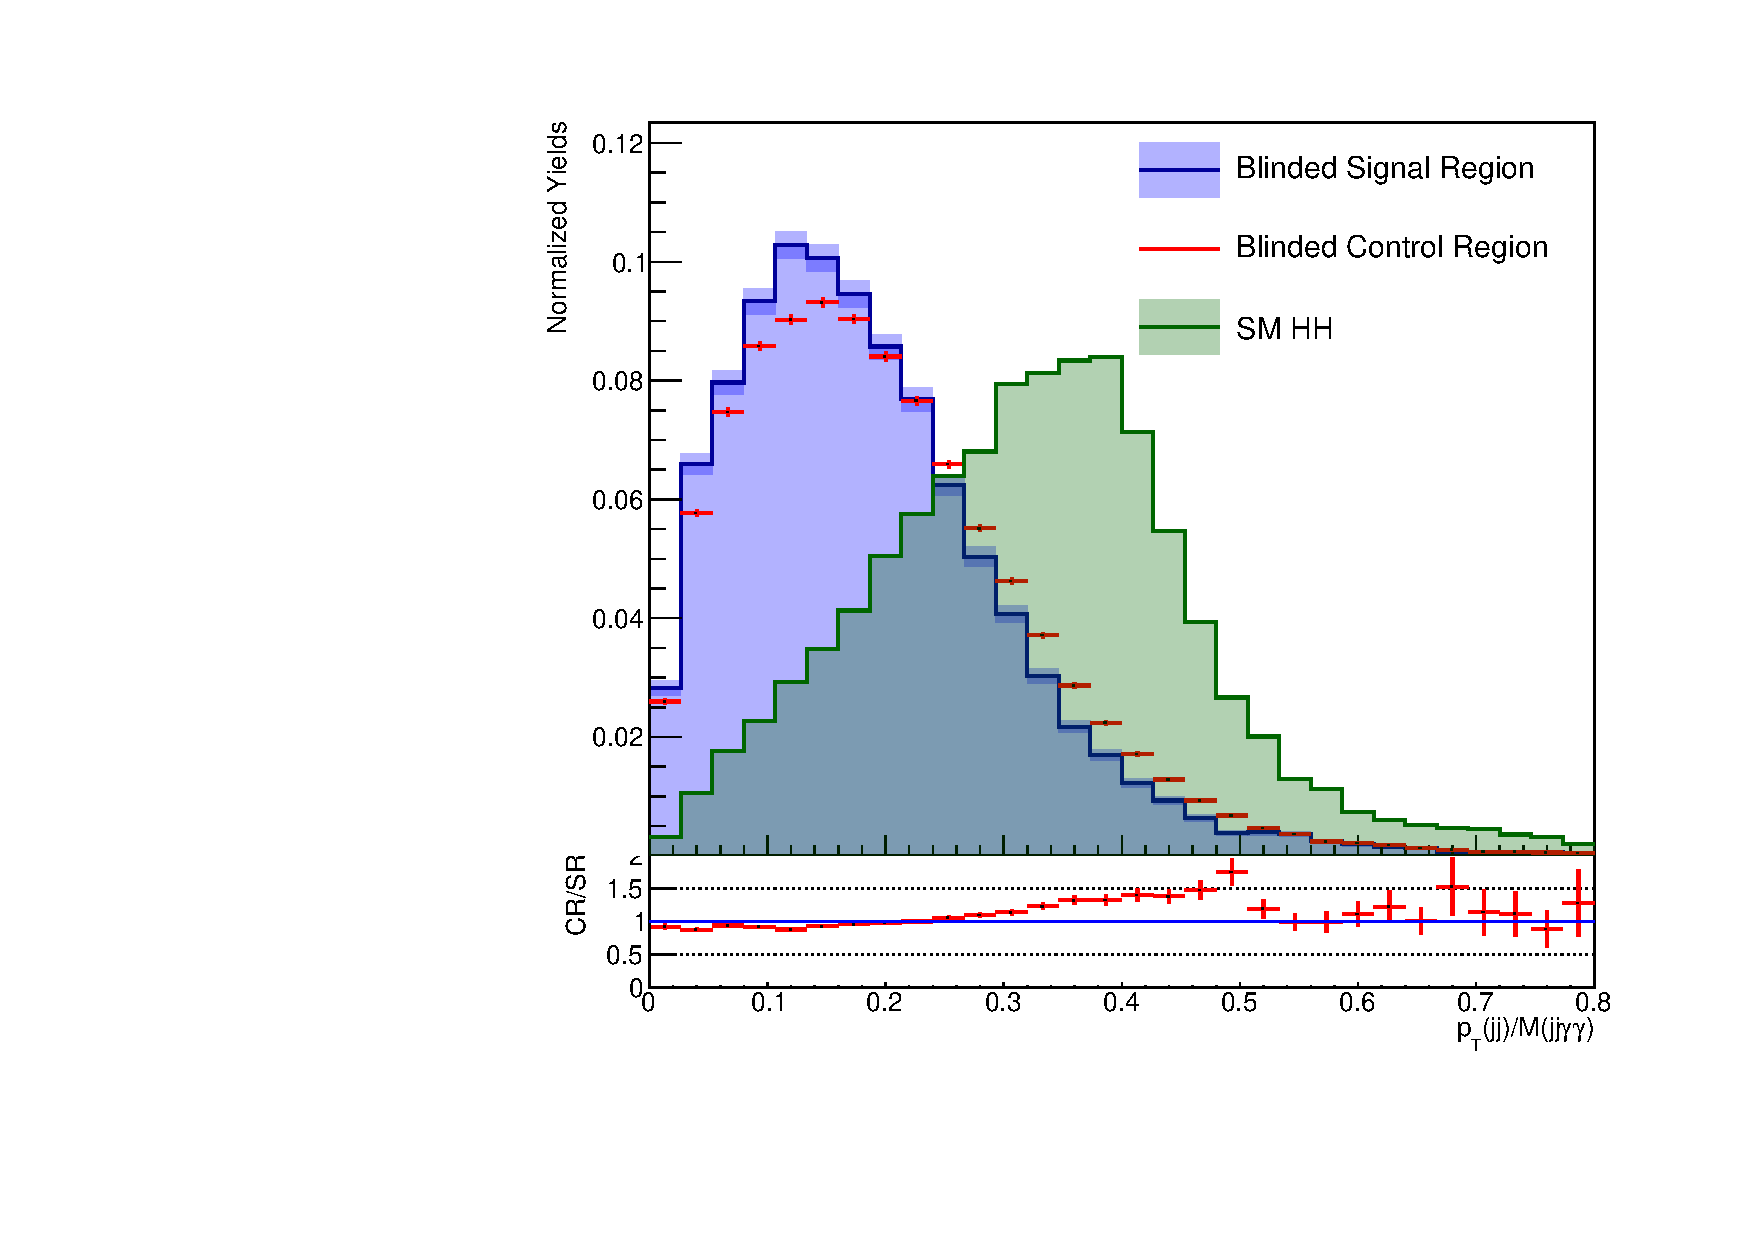
\includegraphics[width=0.3\textwidth]{figures/sec-cats/mva/bbhhr}\hfil
  \caption{Distributions of input variables in the blinded photon control region, blinded signal region, and SM HH sample. All normalized to unity. }
  \label{fig:inputmva}
\end{figure*}

To improve the training, we split the training into two regions: Low Mass and High Mass. 
The low mass training is performed with events with $\tilde{M}_{X}$ below 400 GeV, while the high mass training uses the complementary region. 
The training is based on a decision tree boosted with the gradient algorithm, with the trees randomized between iterations to decrease overtraining. 
To implement the training the TMVA package was used. 
The TMVA output plots are shown for both trainings in Figures \ref{fig:mva_hm} and \ref{fig:mva_lm}. 
From now on, we will refer to the trainings discriminant variable as HHTagger.

With the HHTagger discriminant, we build our two signal categories based on the maximal S/sqrt(B) point, separately in the high mass and in the low mass regions. 
As signal, we use the SM HH sample to calculate the sensitivity. 
The outcome of this study was the categorization in table \ref{tab:catmva}. 
The expected number of background events, when comparing MPC and HPC between cut based and MVA approaches, is comparable and consistent, while for the number of signal events, the performance is better for the HHTagger categorization. 

We have also to insure that the HHTagger selection does not shape our variables of interest, $\Mjj$ and $\Mgg$. 
We demonstrate that there is no appreciable shaping by comparing the $\Mjj$ and $\Mgg$ shapes in different bins of the HHTagger discriminant. 
This can be seen in Figure \ref{fig:mva_mggmjj}. 

\begin{table}
\centering
    \begin{tabular}{| c | c | c |}
    \hline
    Mass Region & HPC & MPC \\ \hline
    Low Mass & HHTagger $> 0.96$ & $ 0.75 < $ HHTagger $ < 0.96 $ \\ \hline 
    High Mass & HHTagger $> 0.96$ & $ 0.6 < $ HHTagger $ < 0.96 $ \\ \hline 
    \end{tabular}
\caption{Non-resonant categorization with HHTagger discriminant.}
\label{tab:catmva}
\end{table}


\begin{figure*}[thb]
  \centering
  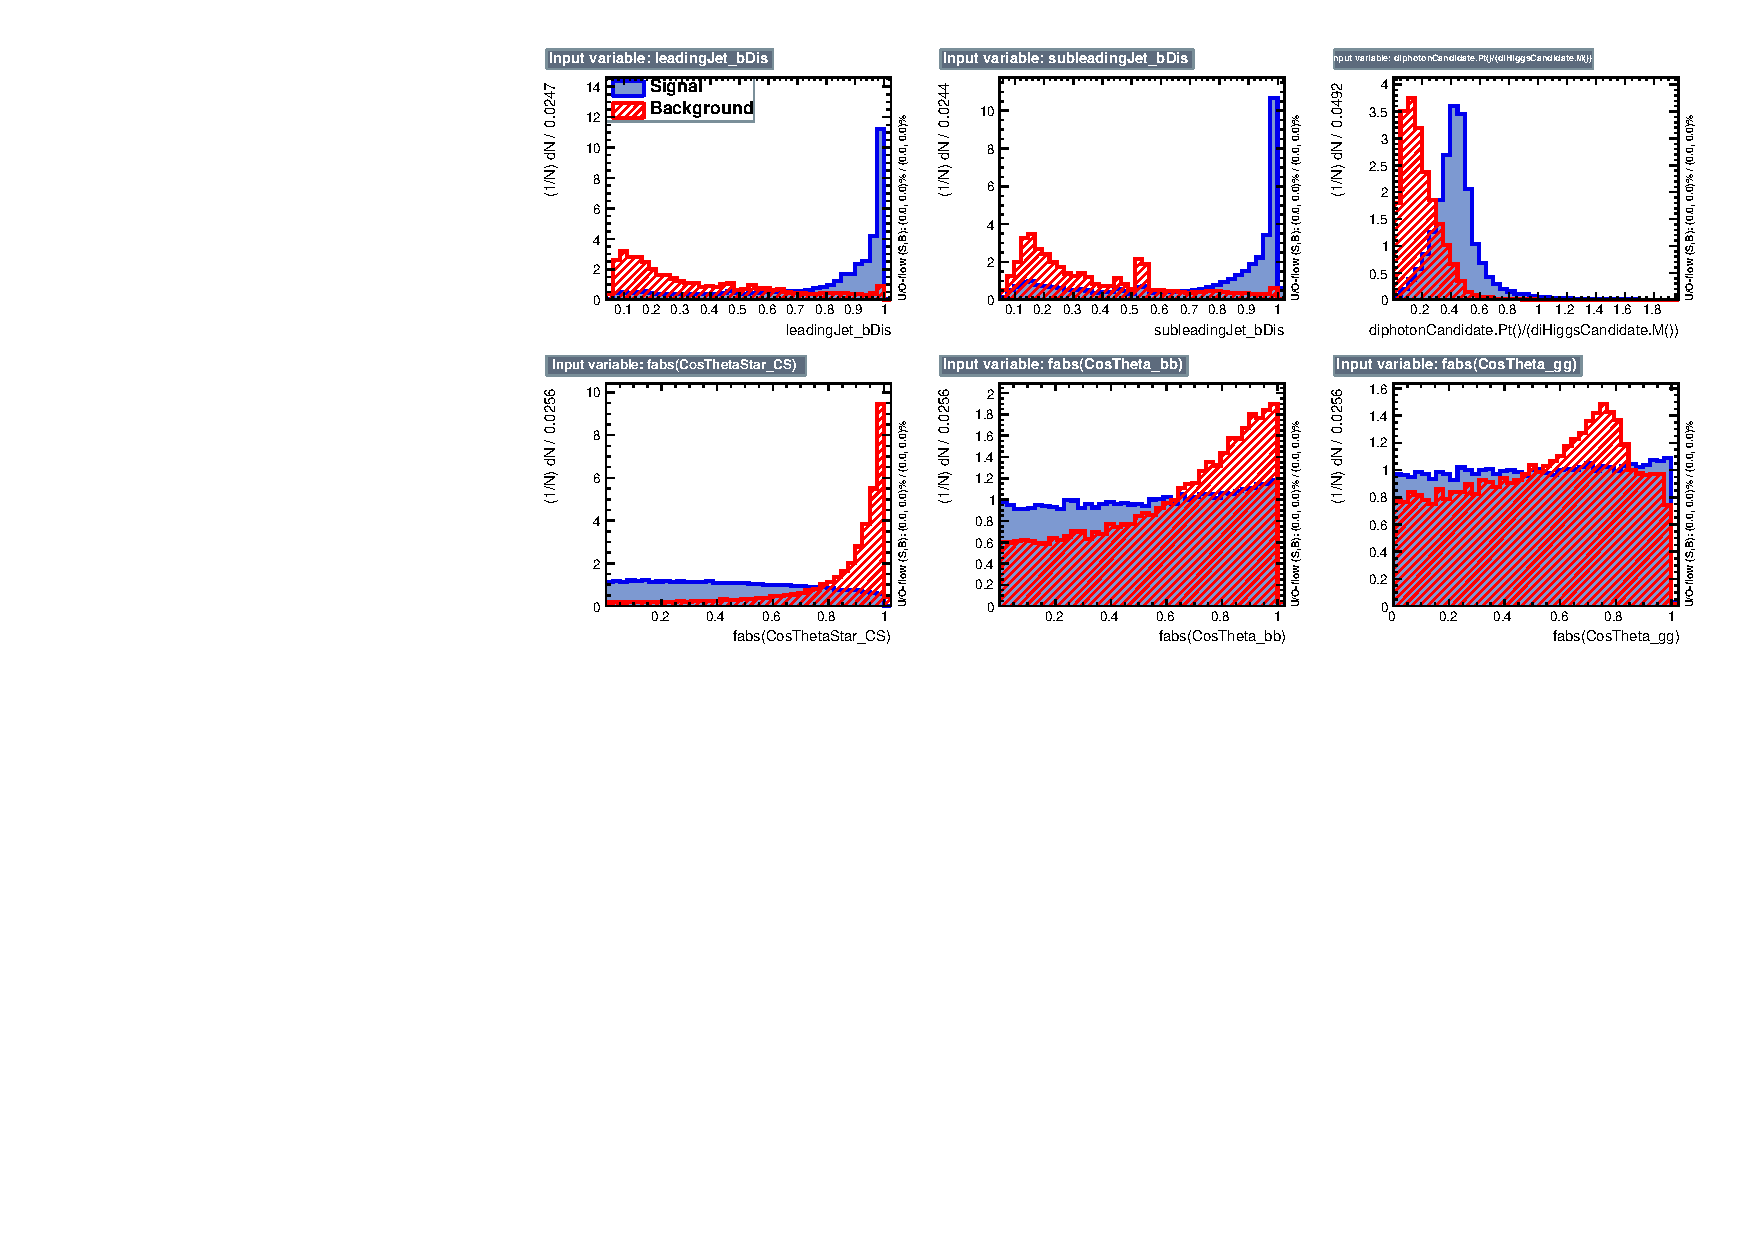
\includegraphics[width=0.45\textwidth]{figures/sec-cats/mva/vars1_hm400}\hfil
  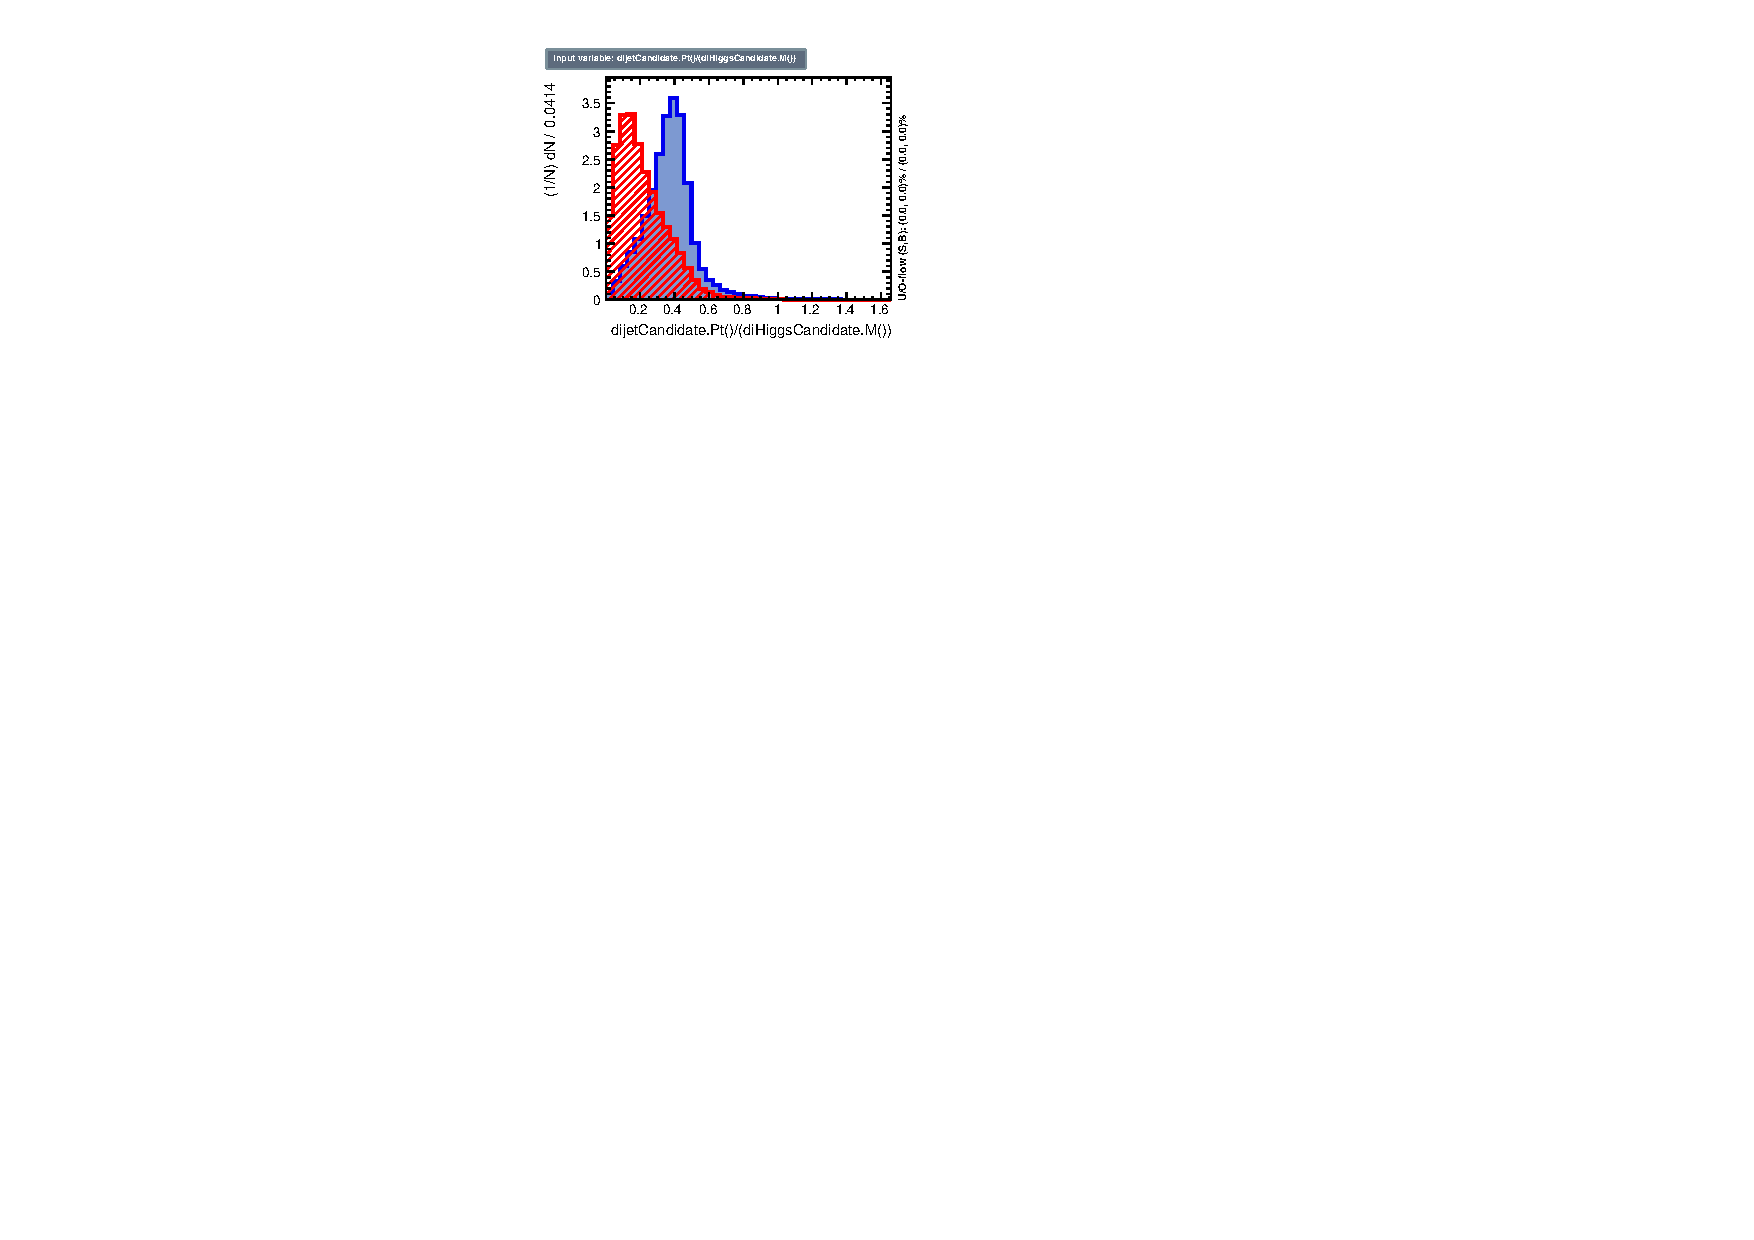
\includegraphics[width=0.45\textwidth]{figures/sec-cats/mva/vars2_hm400}\hfil
  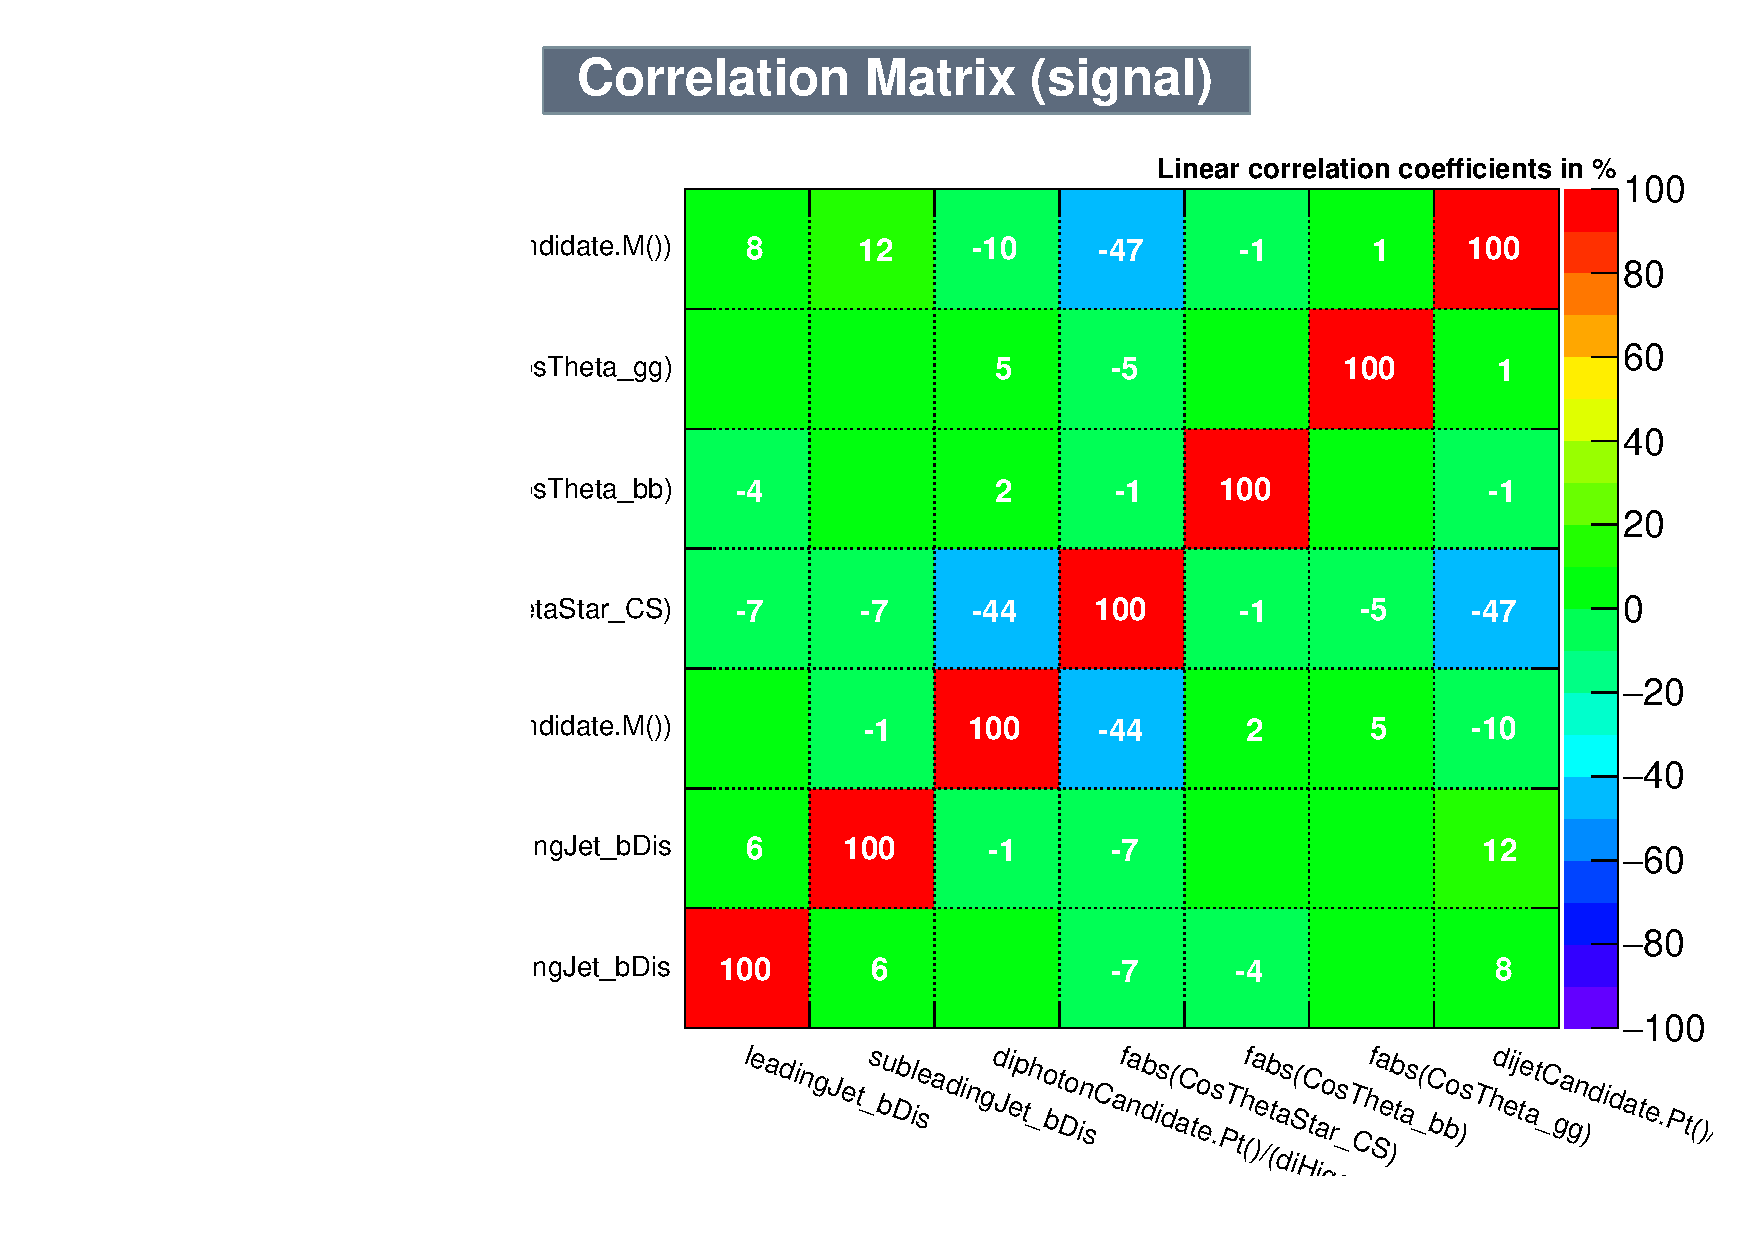
\includegraphics[width=0.45\textwidth]{figures/sec-cats/mva/corsS_hm400}\hfil
  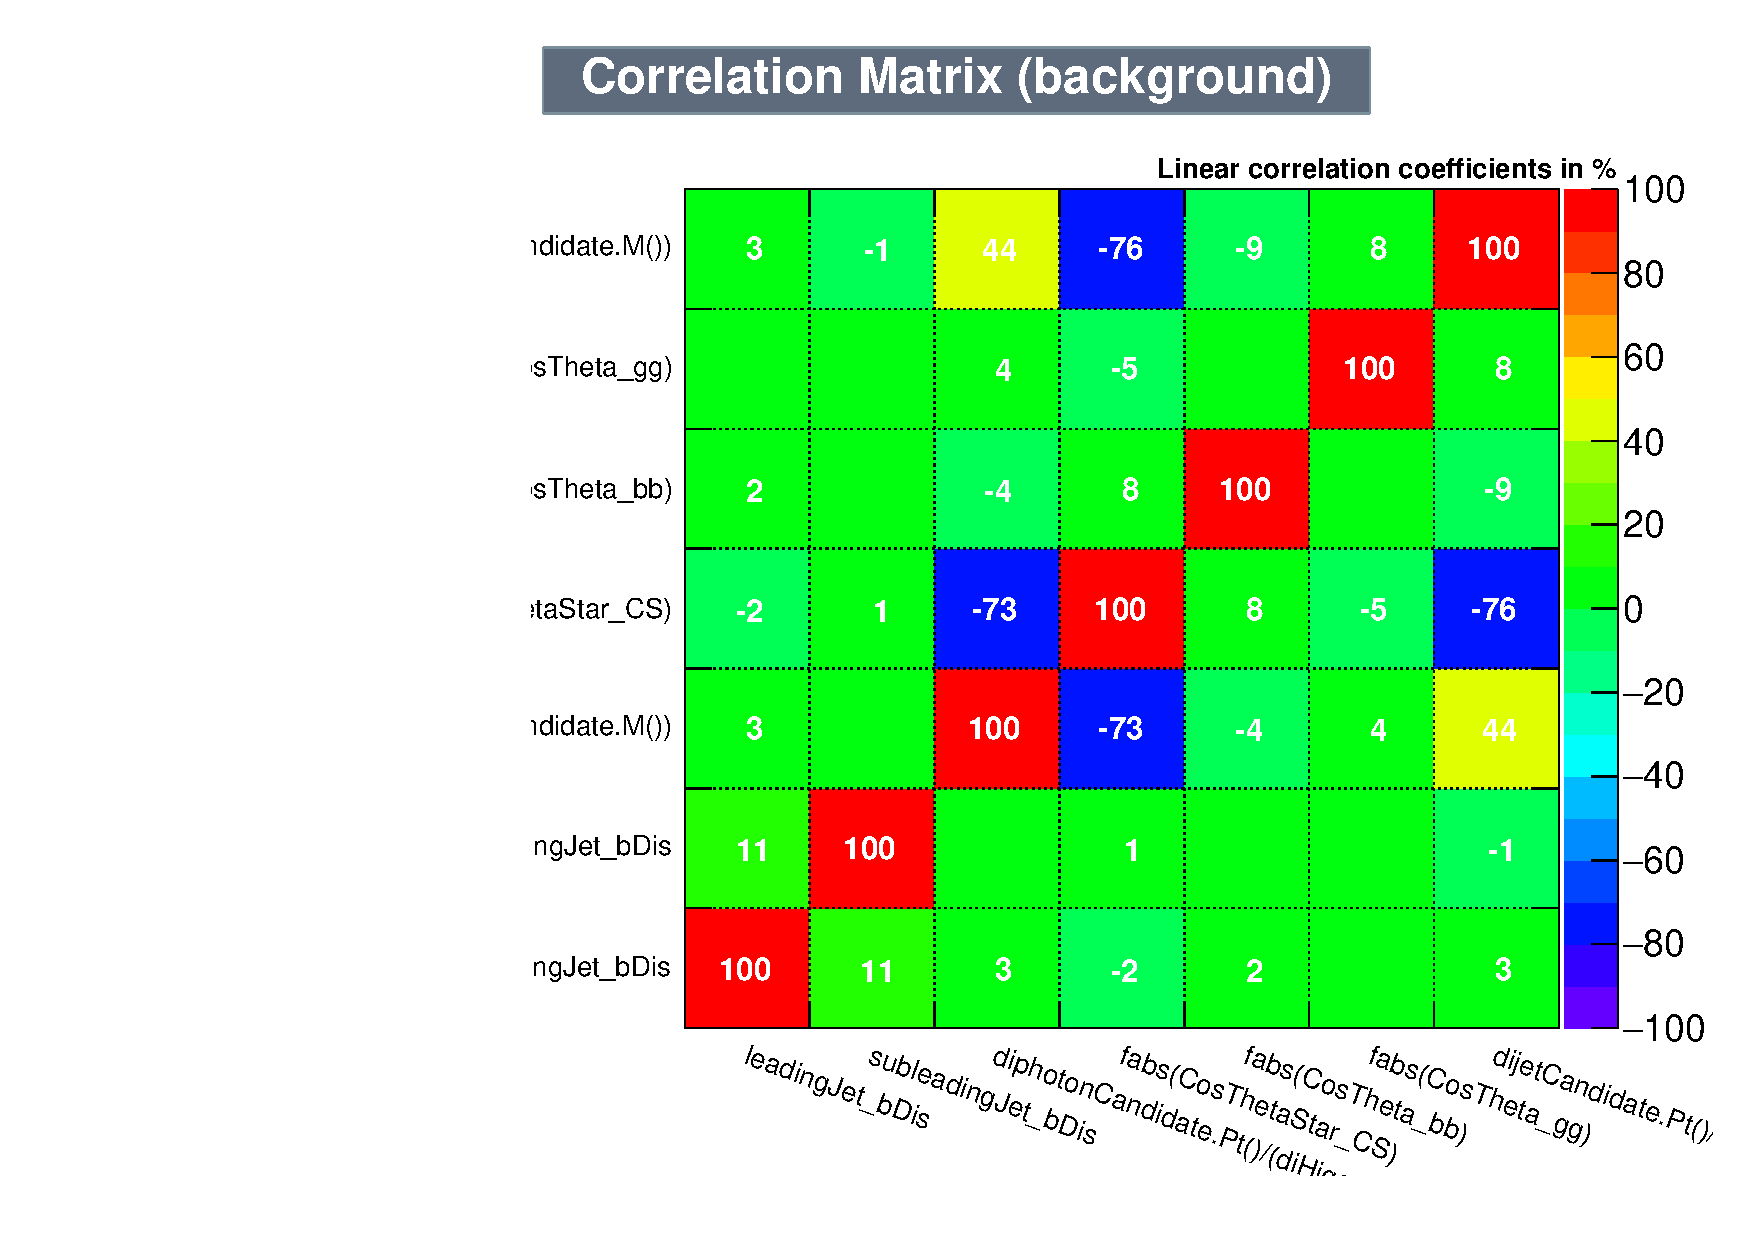
\includegraphics[width=0.45\textwidth]{figures/sec-cats/mva/corsB_hm400}\hfil
  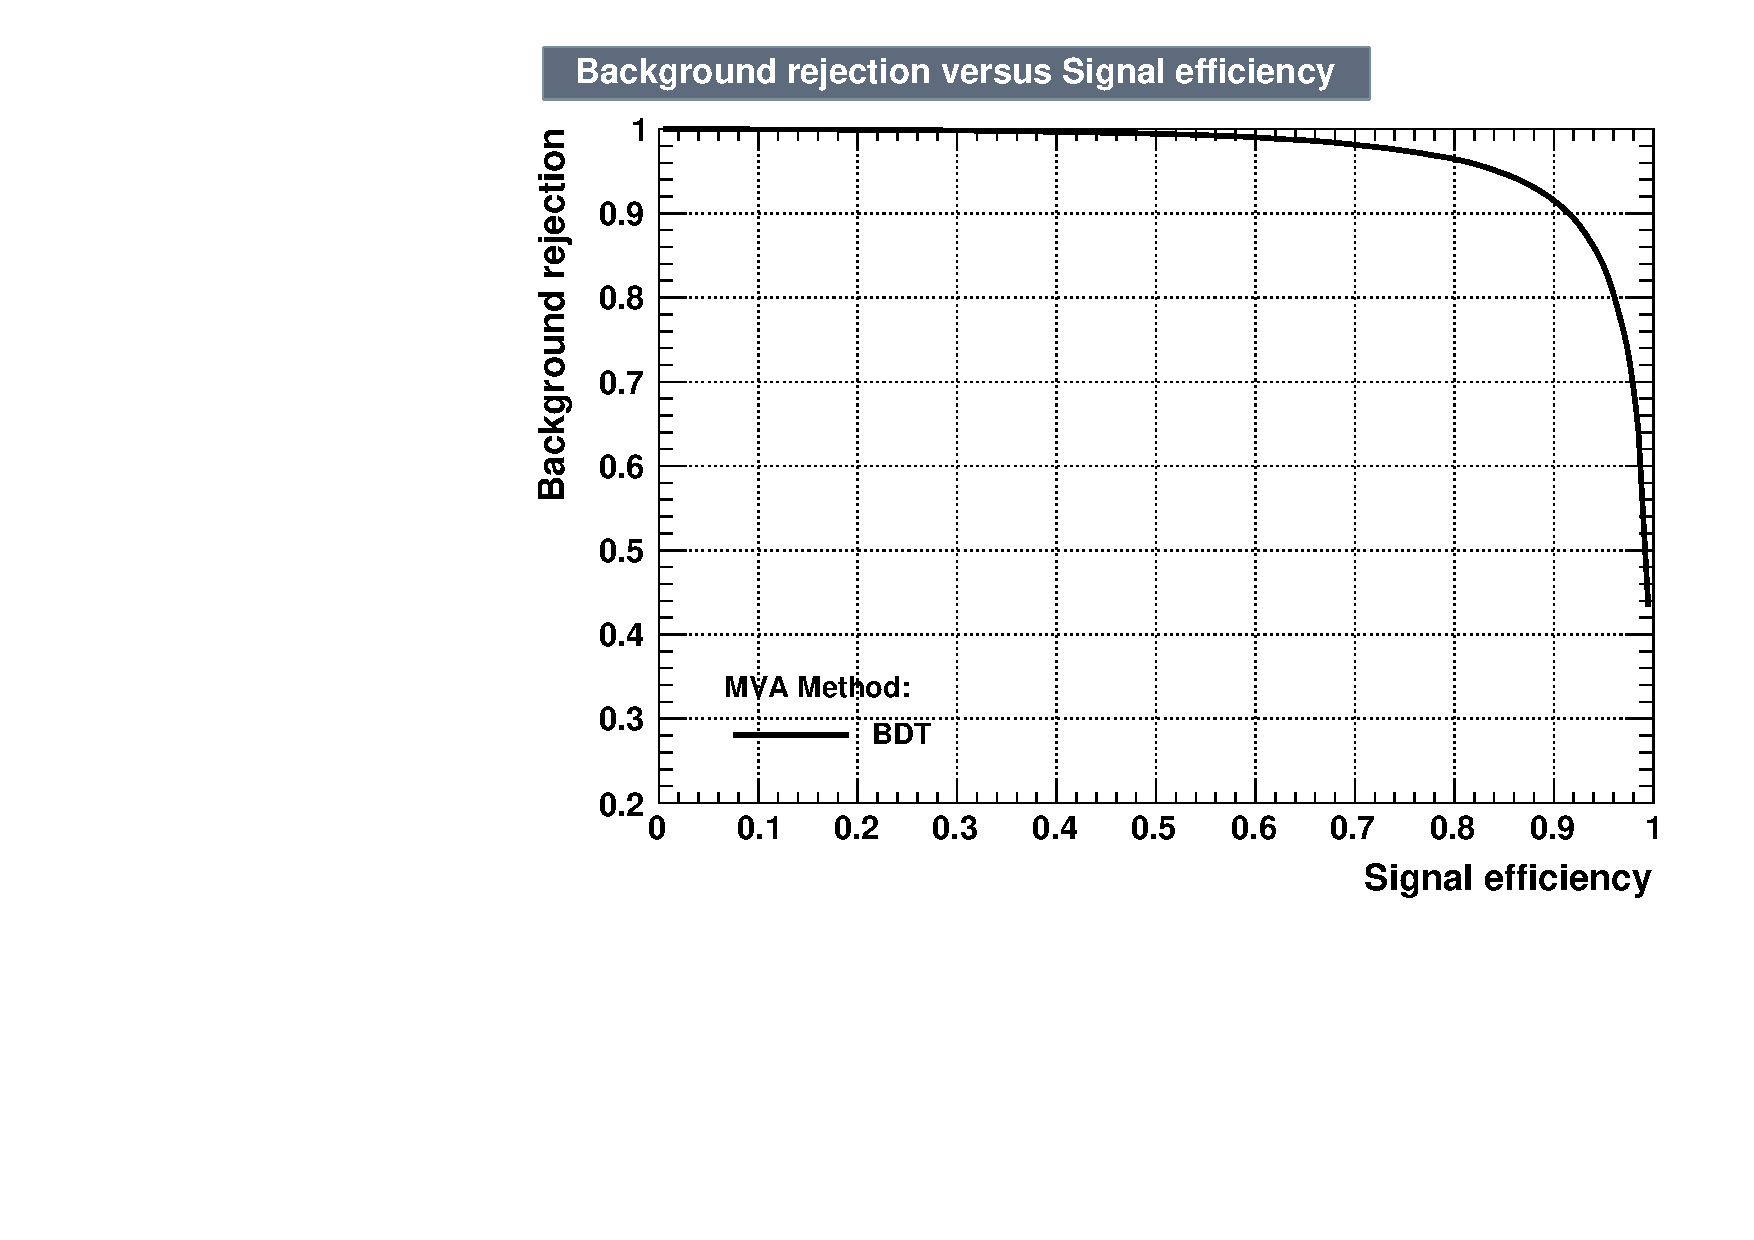
\includegraphics[width=0.45\textwidth]{figures/sec-cats/mva/ROC_hm400}\hfil
  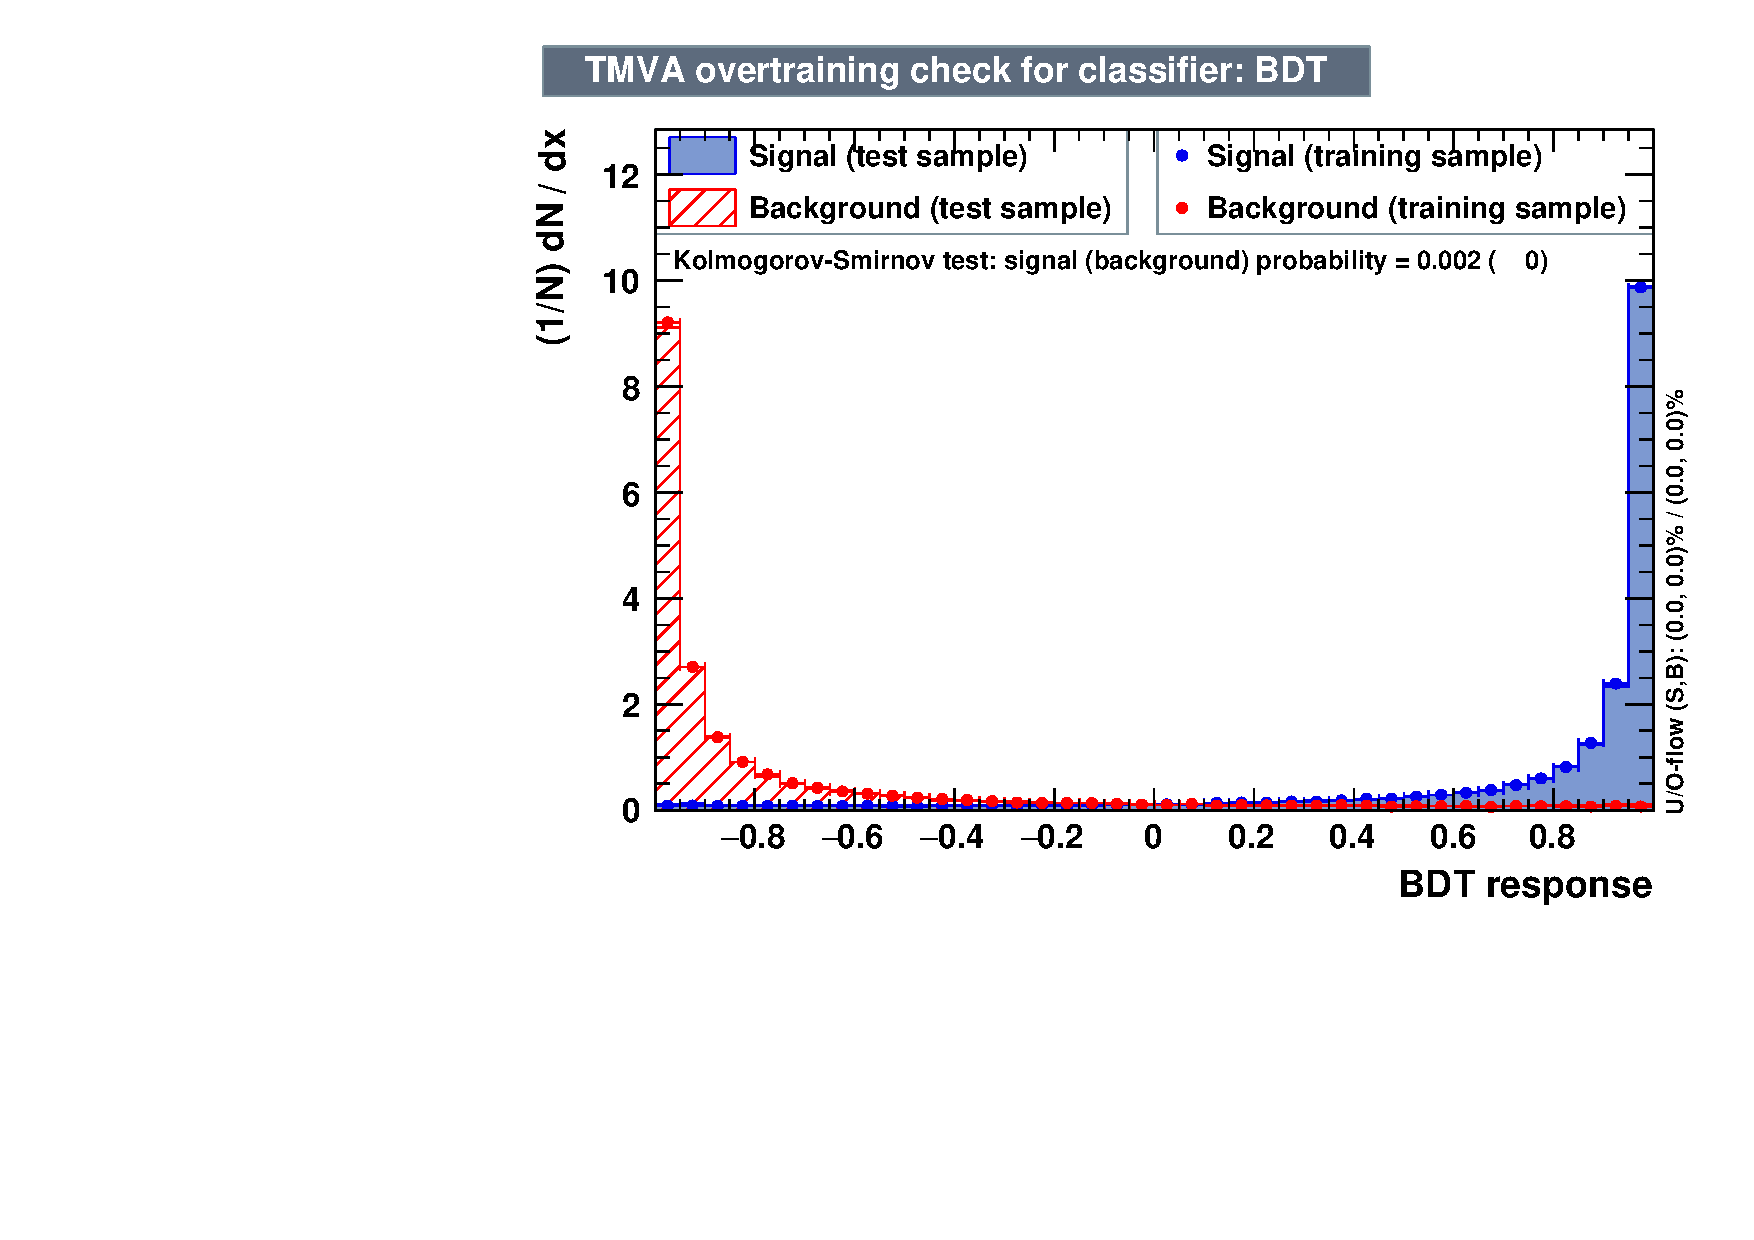
\includegraphics[width=0.45\textwidth]{figures/sec-cats/mva/discr_hm400}\hfil
  \caption{TMVA output plots for the High Mass Training.}
  \label{fig:mva_hm}
\end{figure*}

\begin{figure*}[thb]
  \centering
  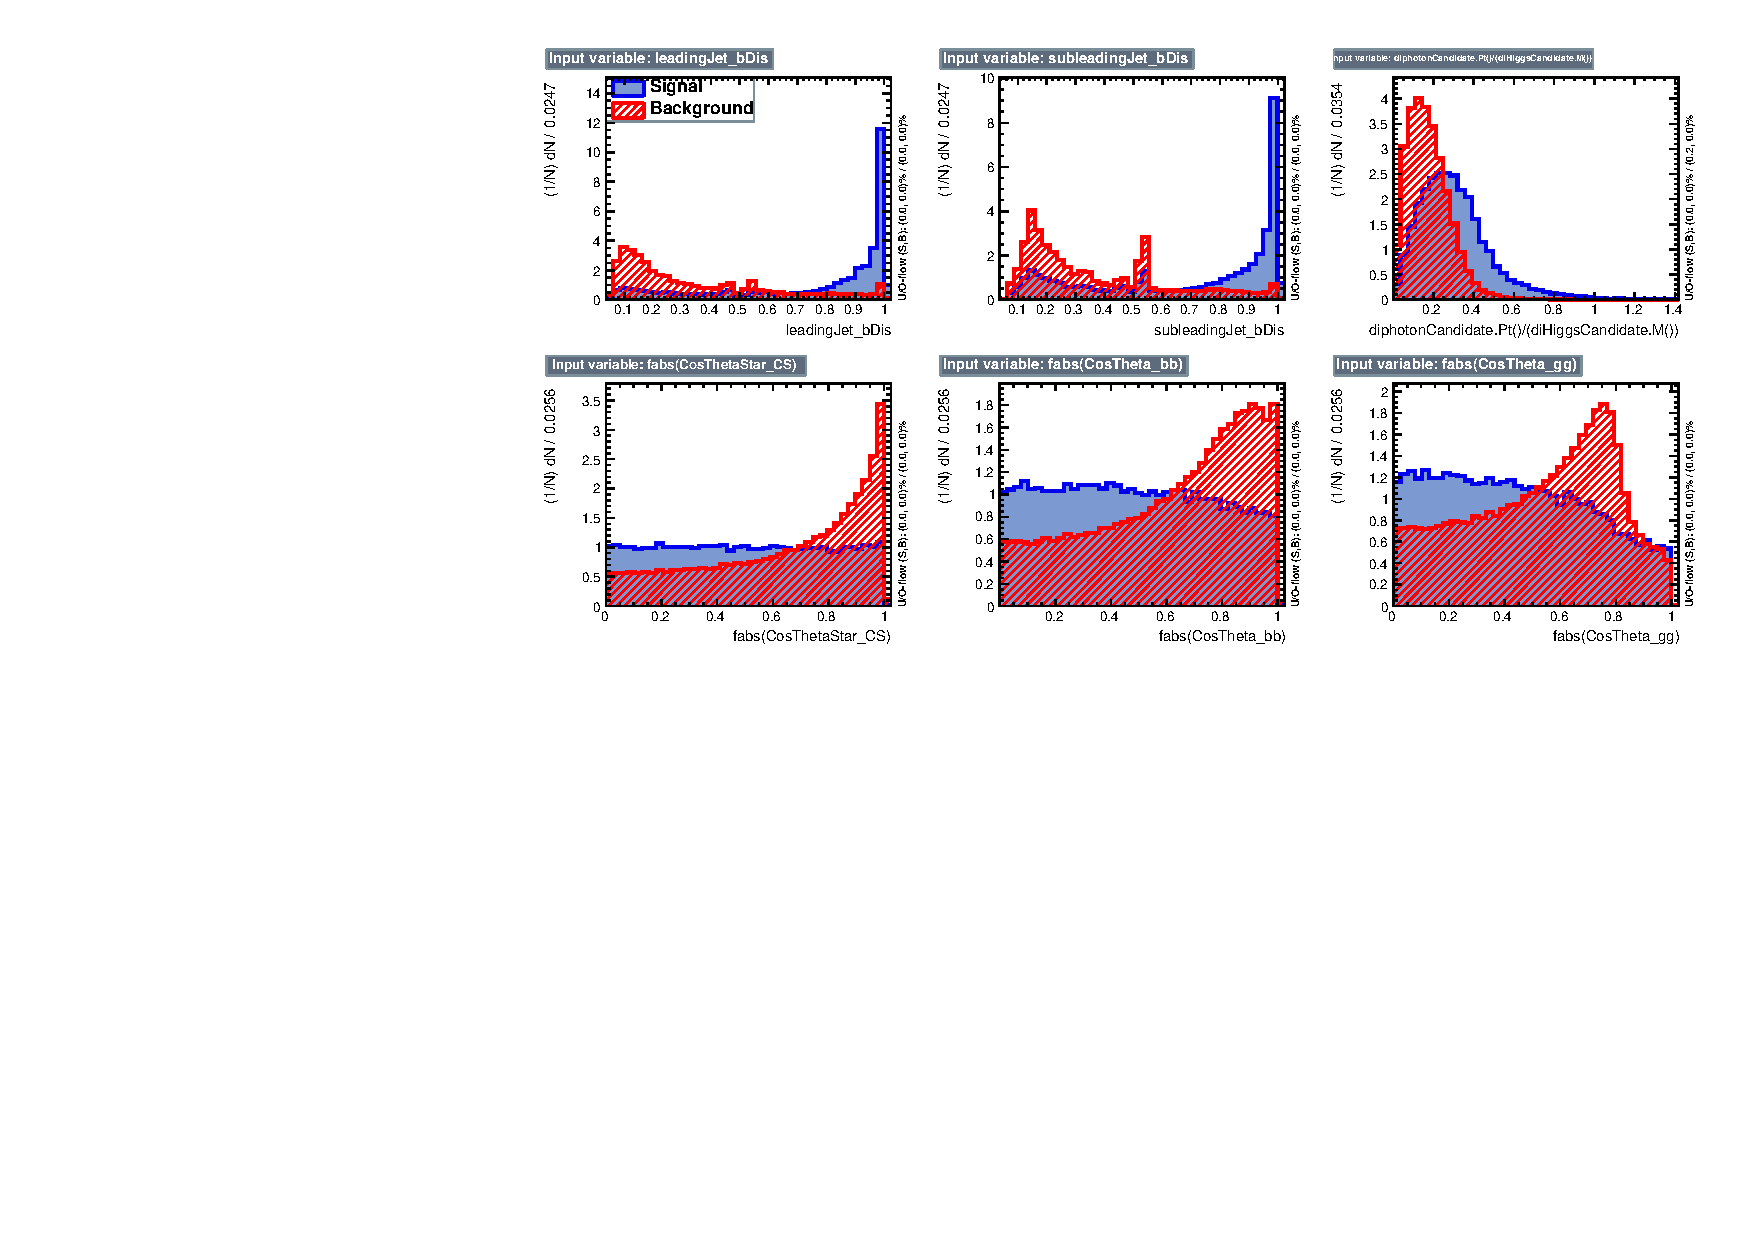
\includegraphics[width=0.45\textwidth]{figures/sec-cats/mva/vars1_lm400}\hfil
  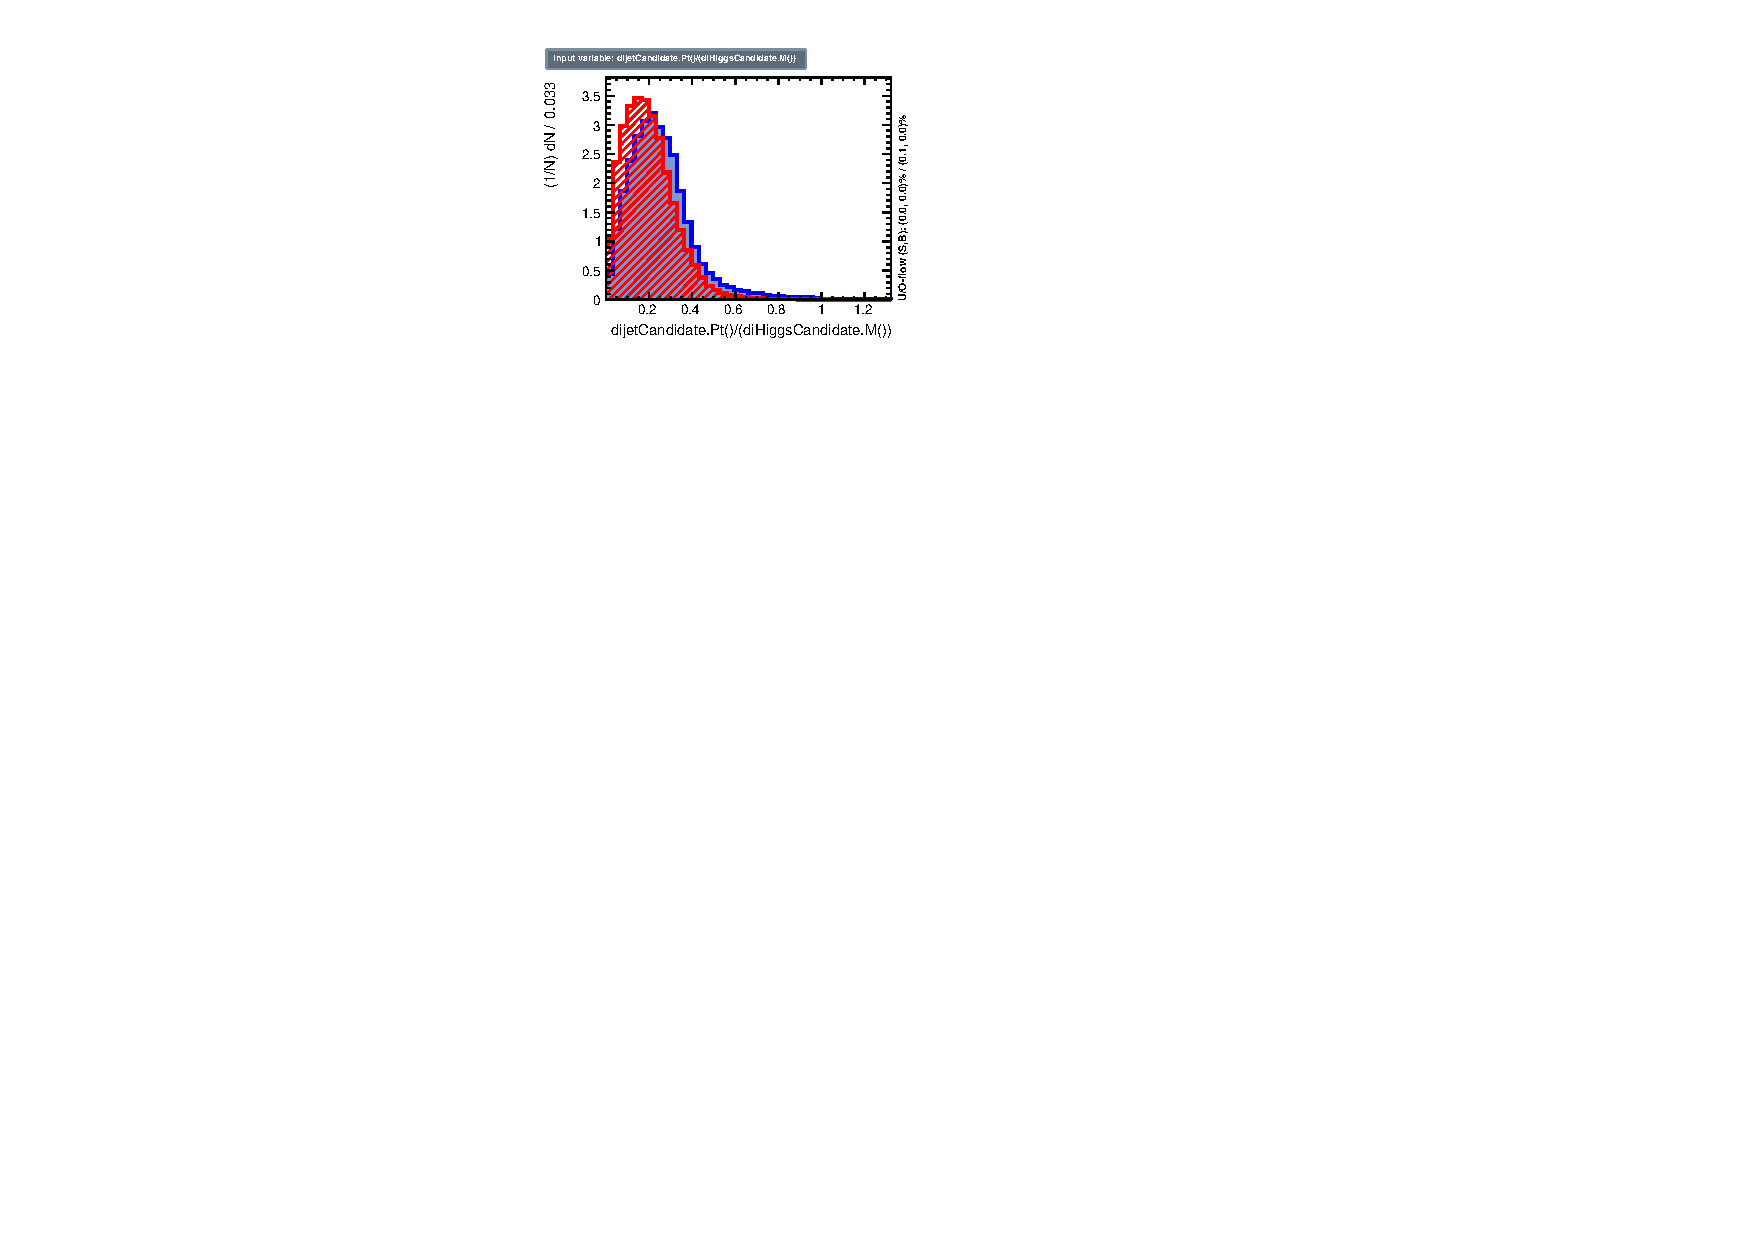
\includegraphics[width=0.45\textwidth]{figures/sec-cats/mva/vars2_lm400}\hfil
  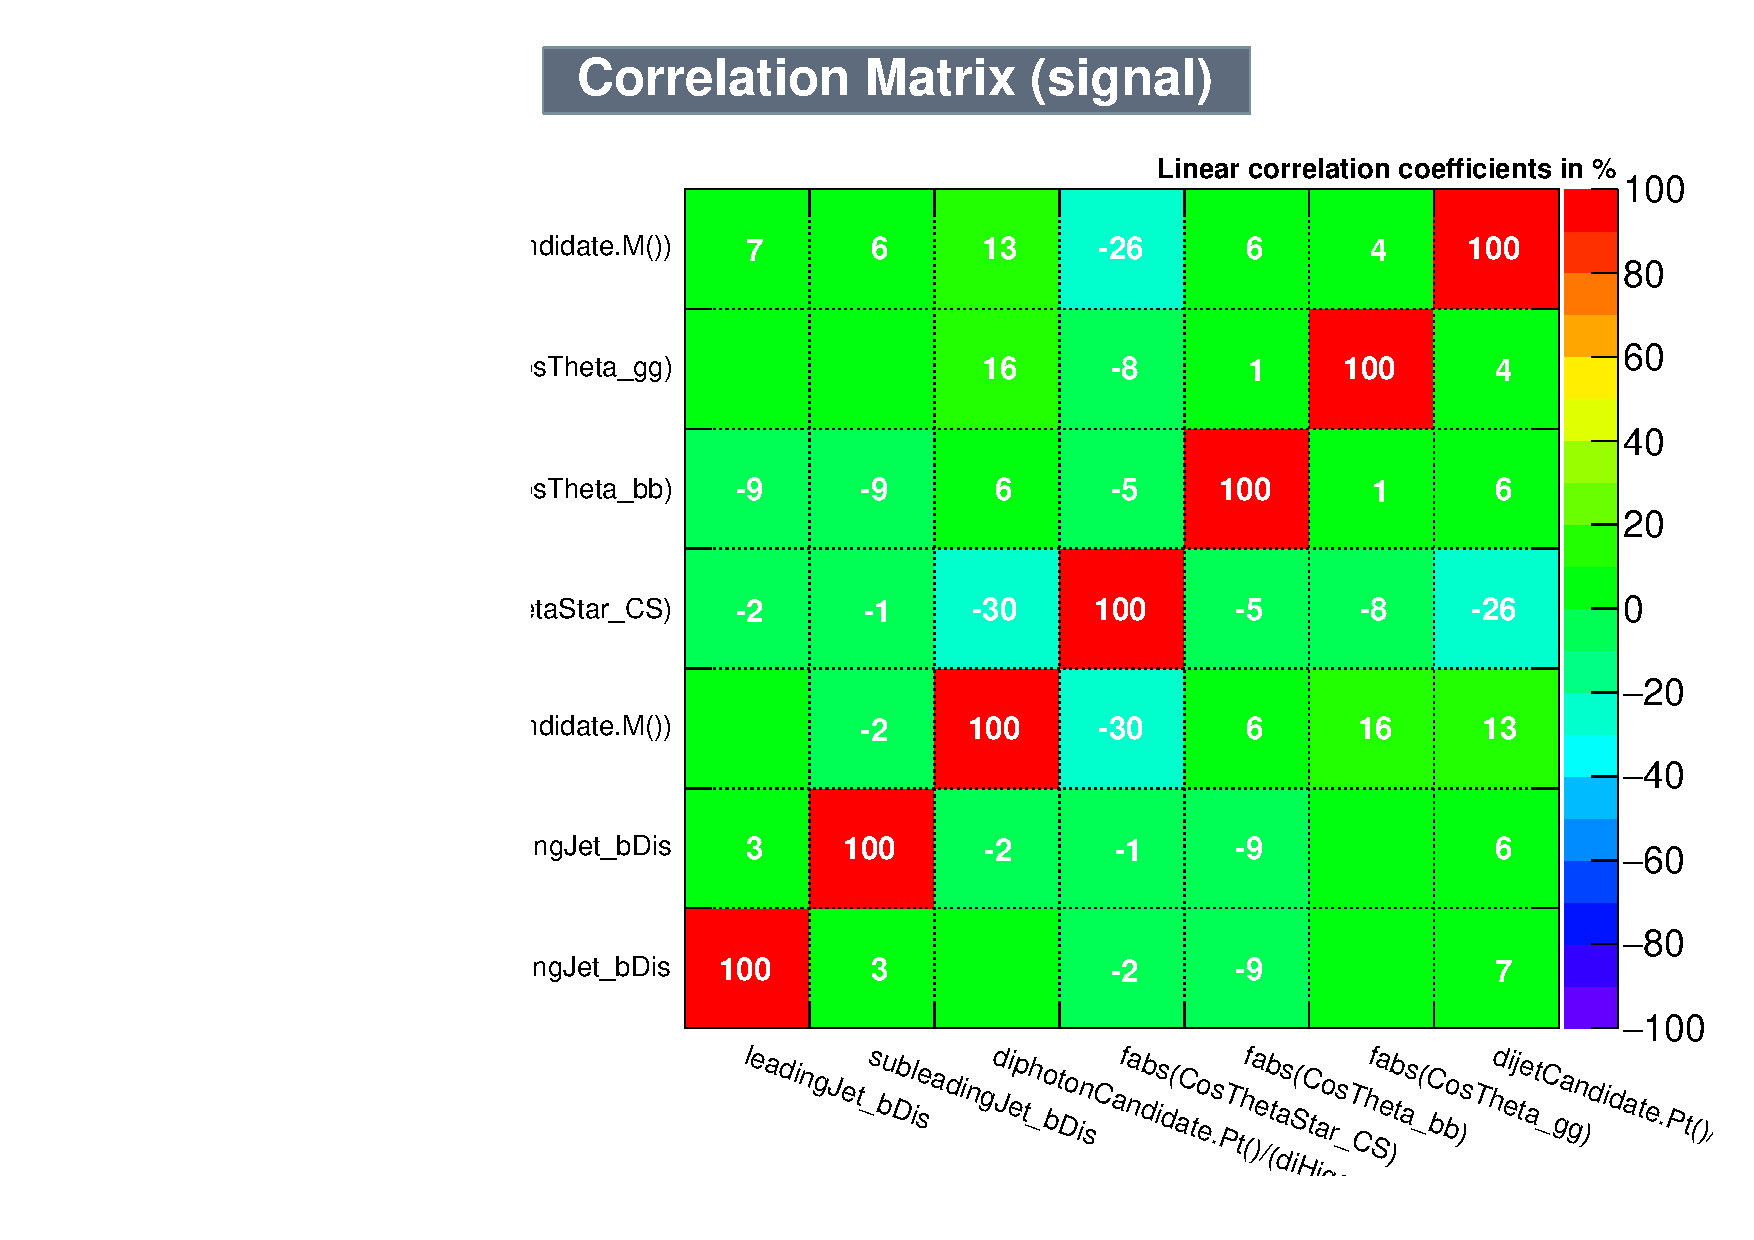
\includegraphics[width=0.45\textwidth]{figures/sec-cats/mva/corsS_lm400}\hfil
  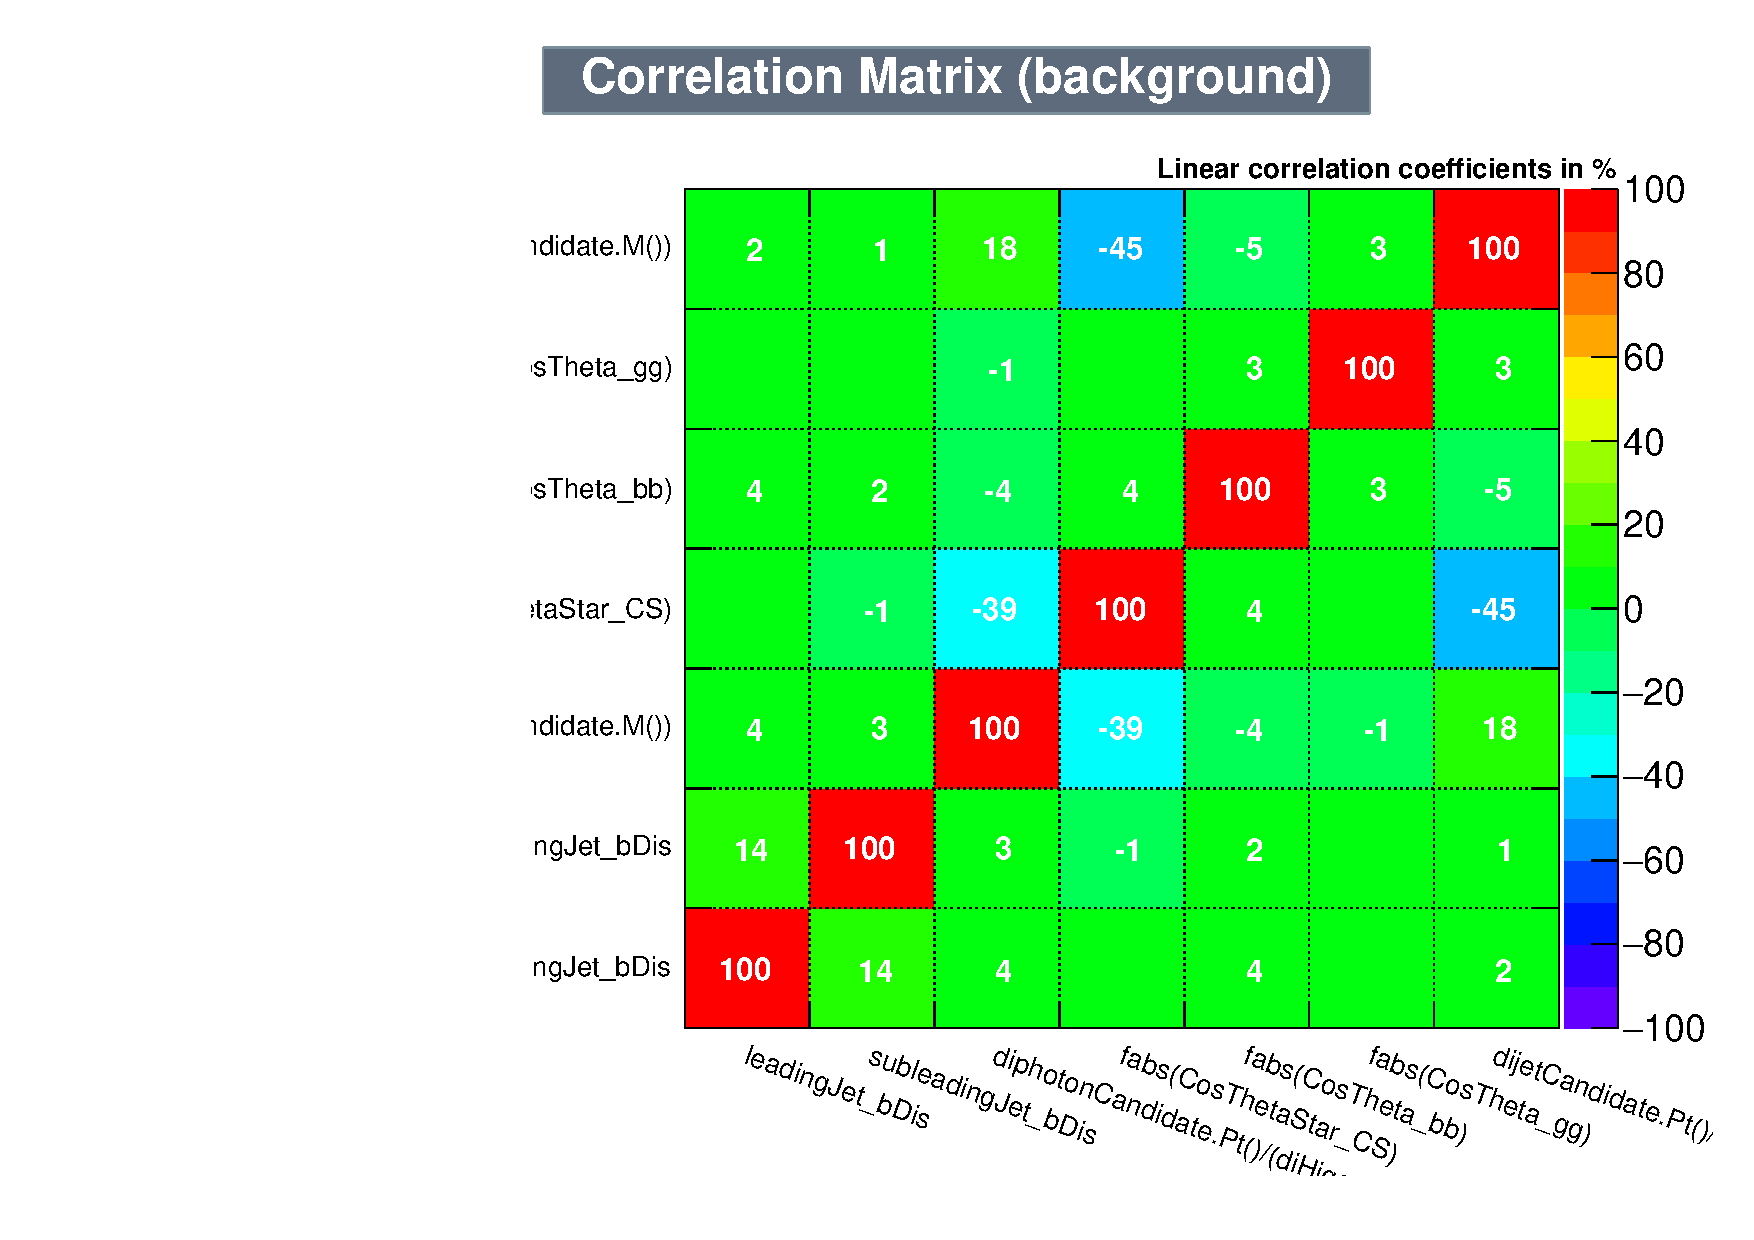
\includegraphics[width=0.45\textwidth]{figures/sec-cats/mva/corsB_lm400}\hfil
  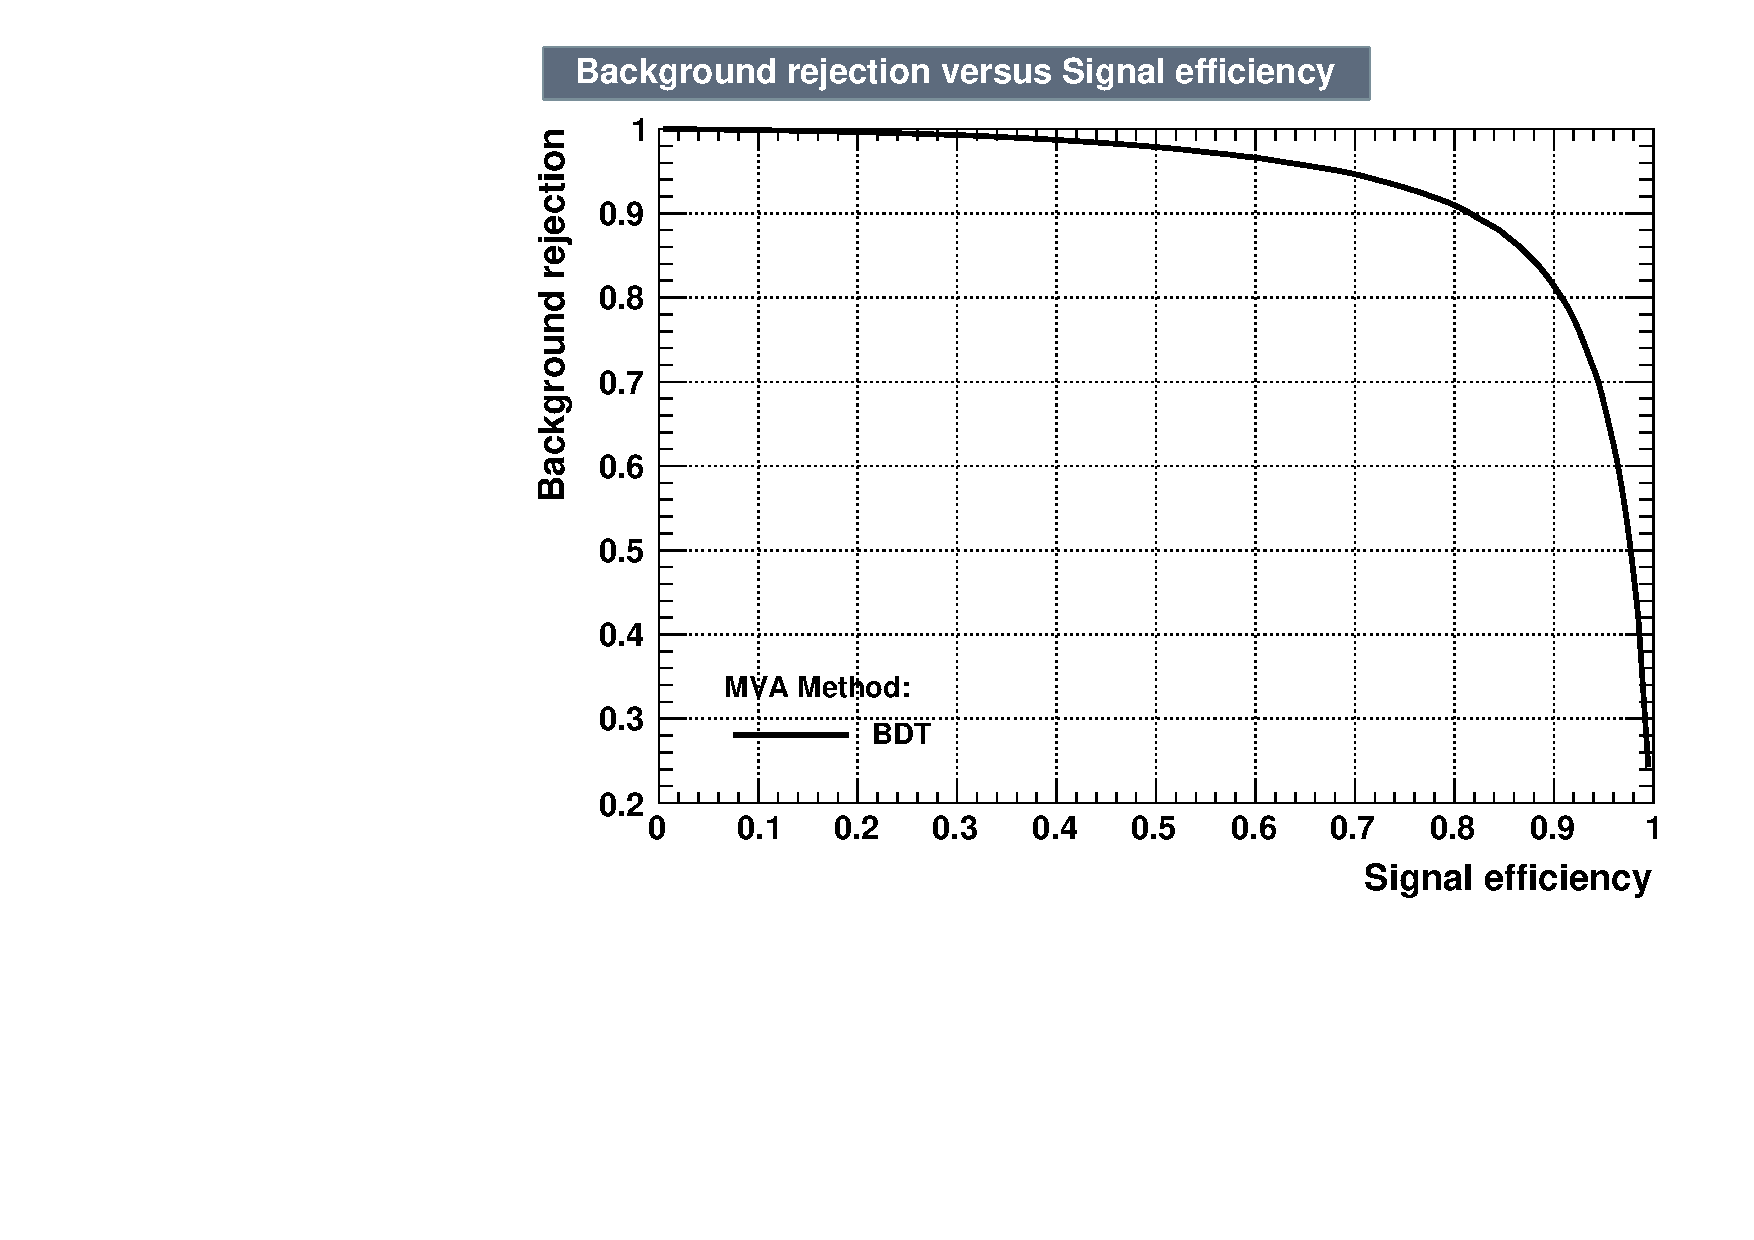
\includegraphics[width=0.45\textwidth]{figures/sec-cats/mva/ROC_lm400}\hfil
  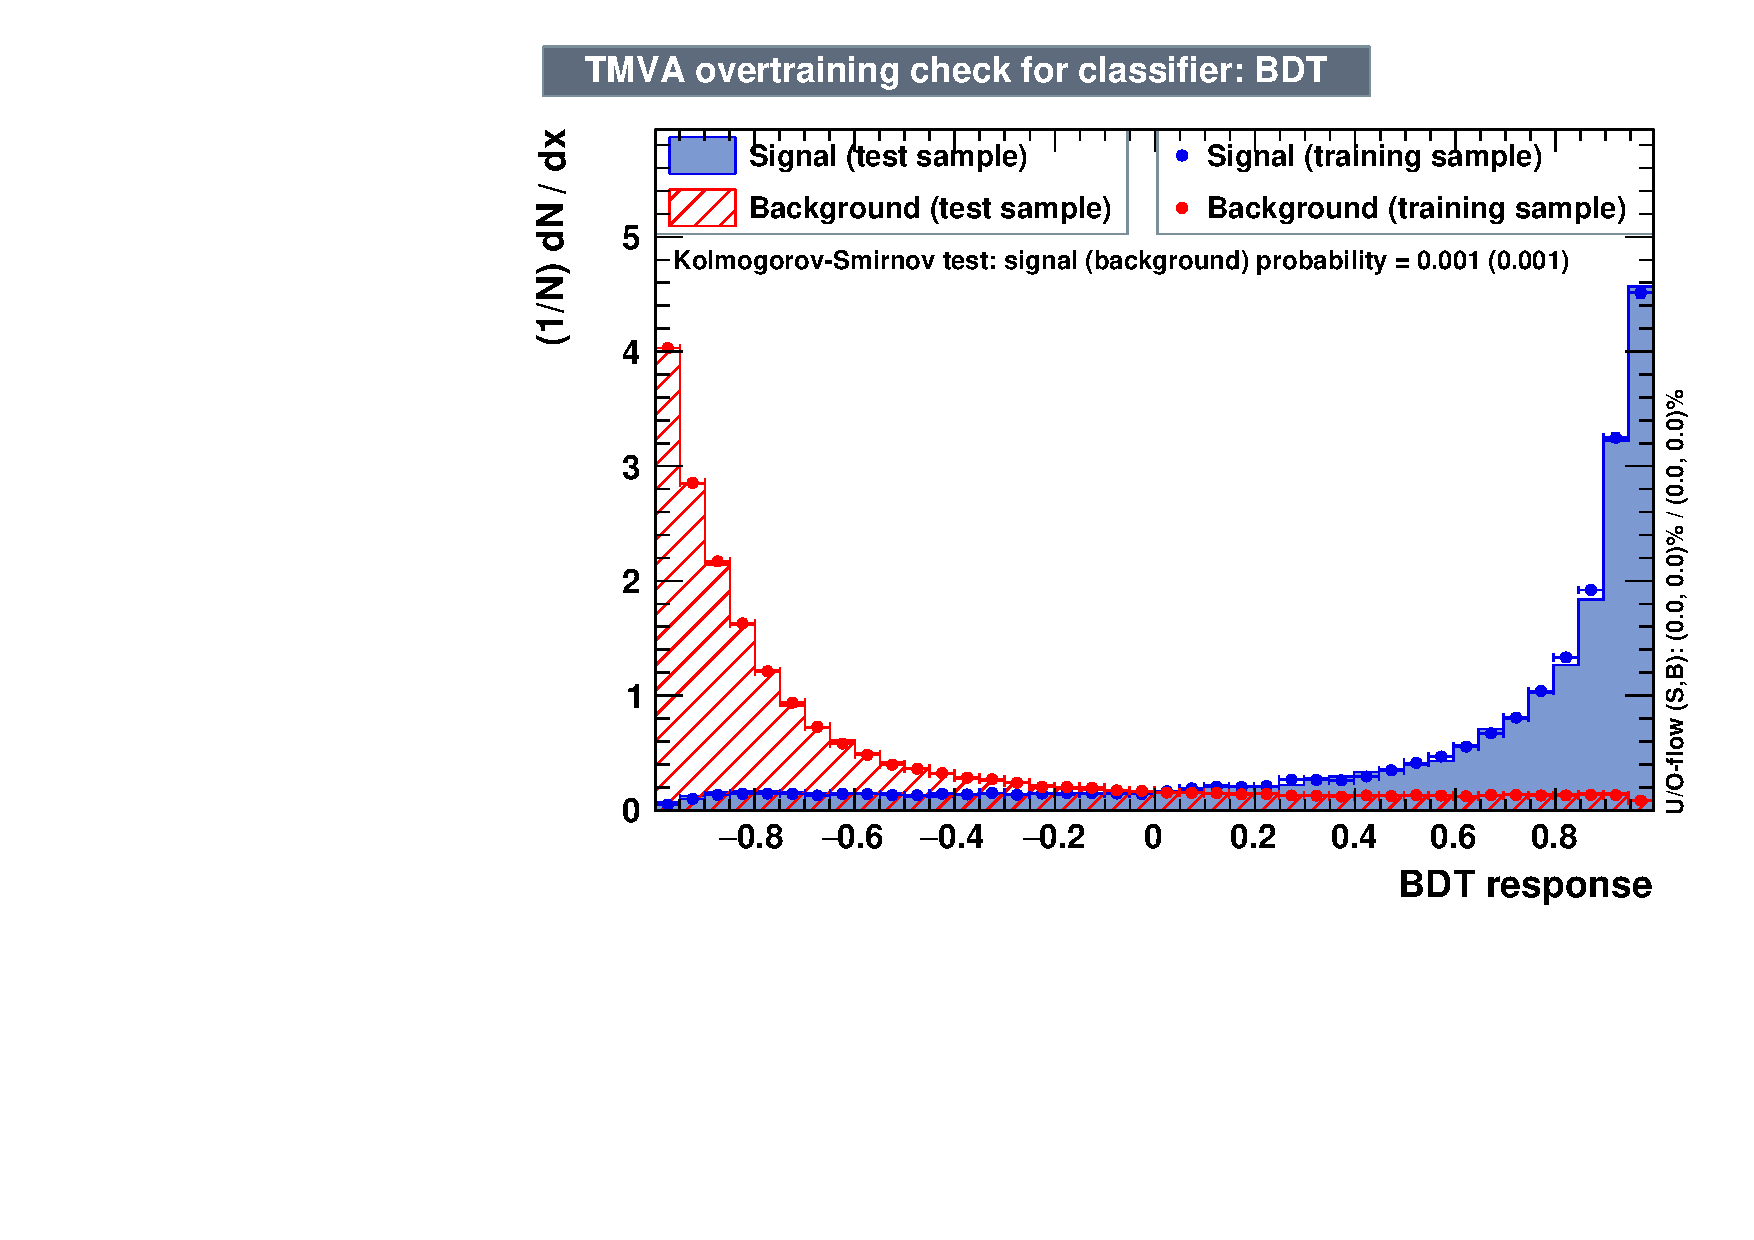
\includegraphics[width=0.45\textwidth]{figures/sec-cats/mva/discr_lm400}\hfil
  \caption{TMVA output plots for the Low Mass Training.}
  \label{fig:mva_lm}
\end{figure*}

\begin{figure*}[thb]
  \centering
  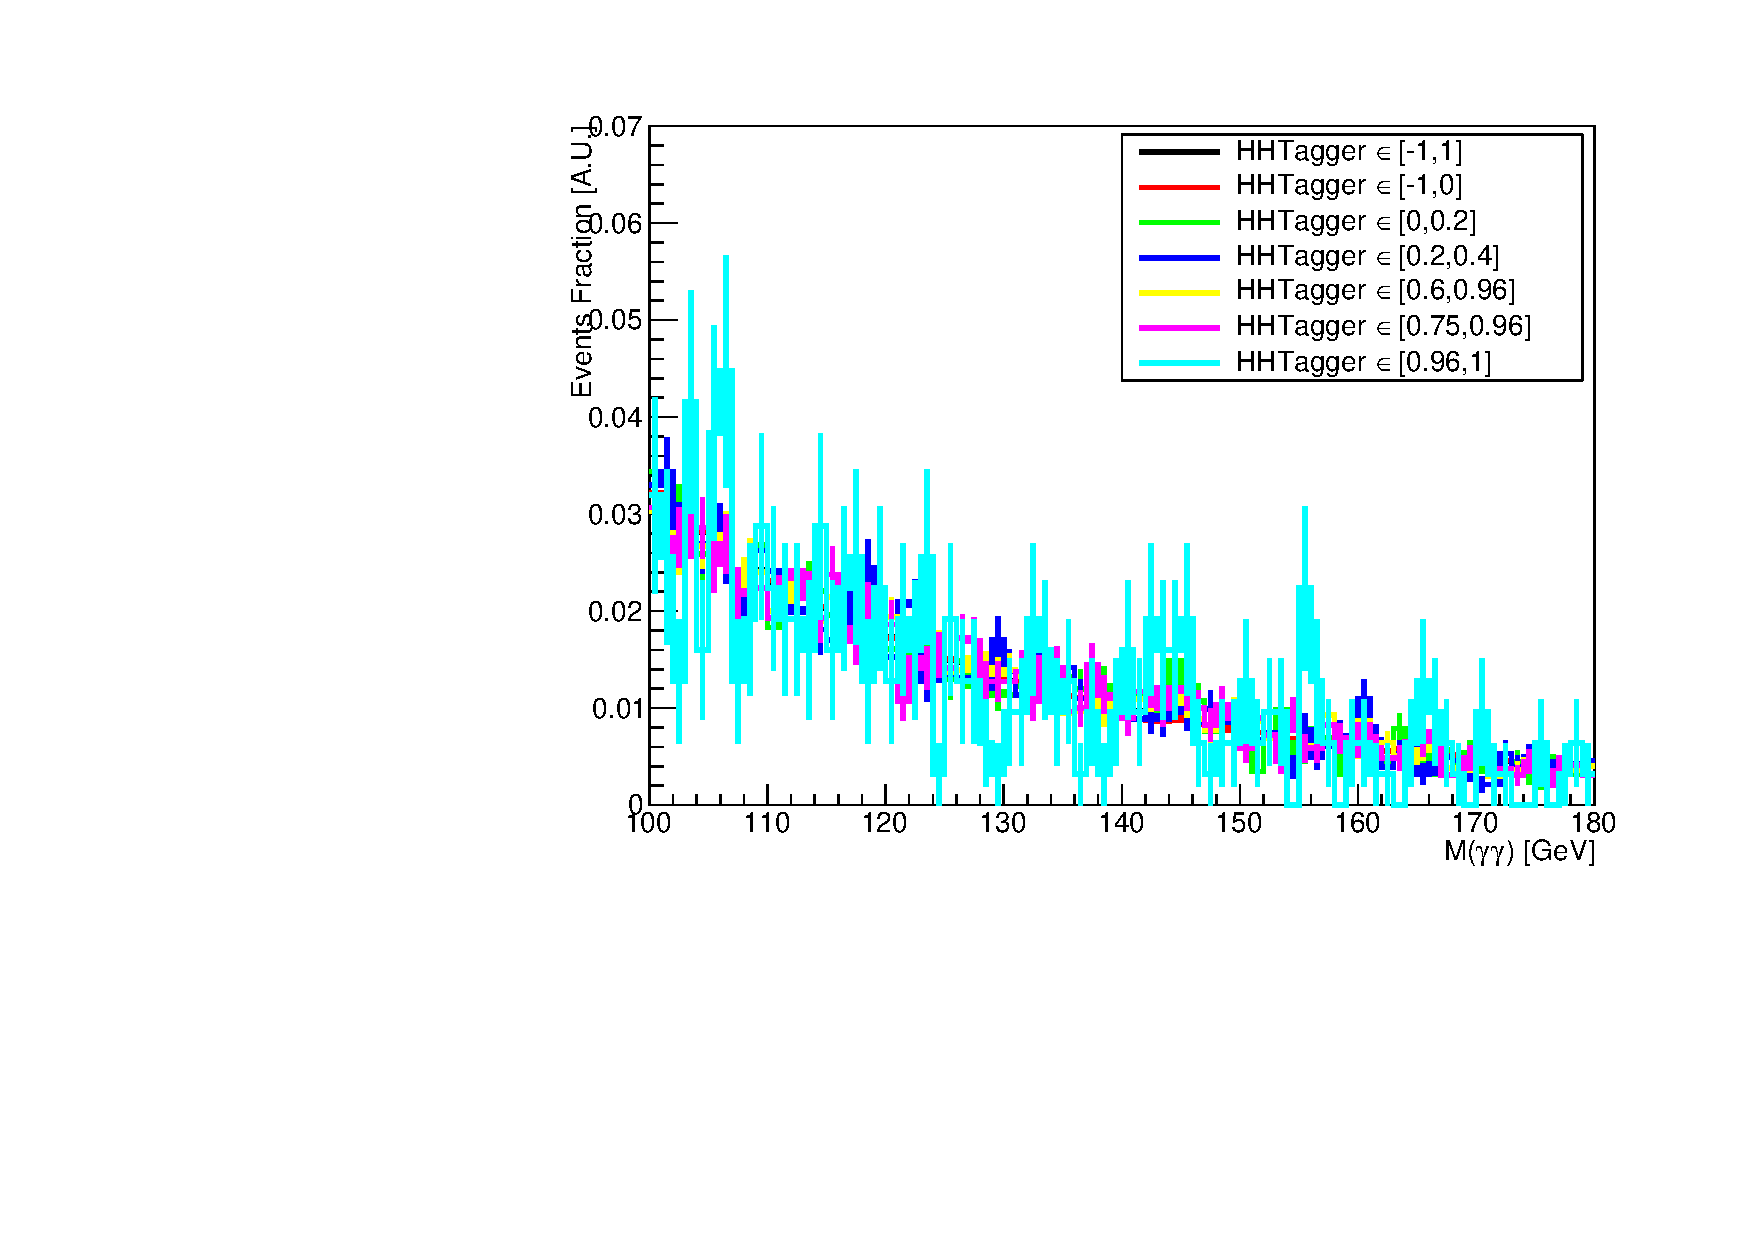
\includegraphics[width=0.45\textwidth]{figures/sec-cats/mva/hhtag_mgg}\hfil
  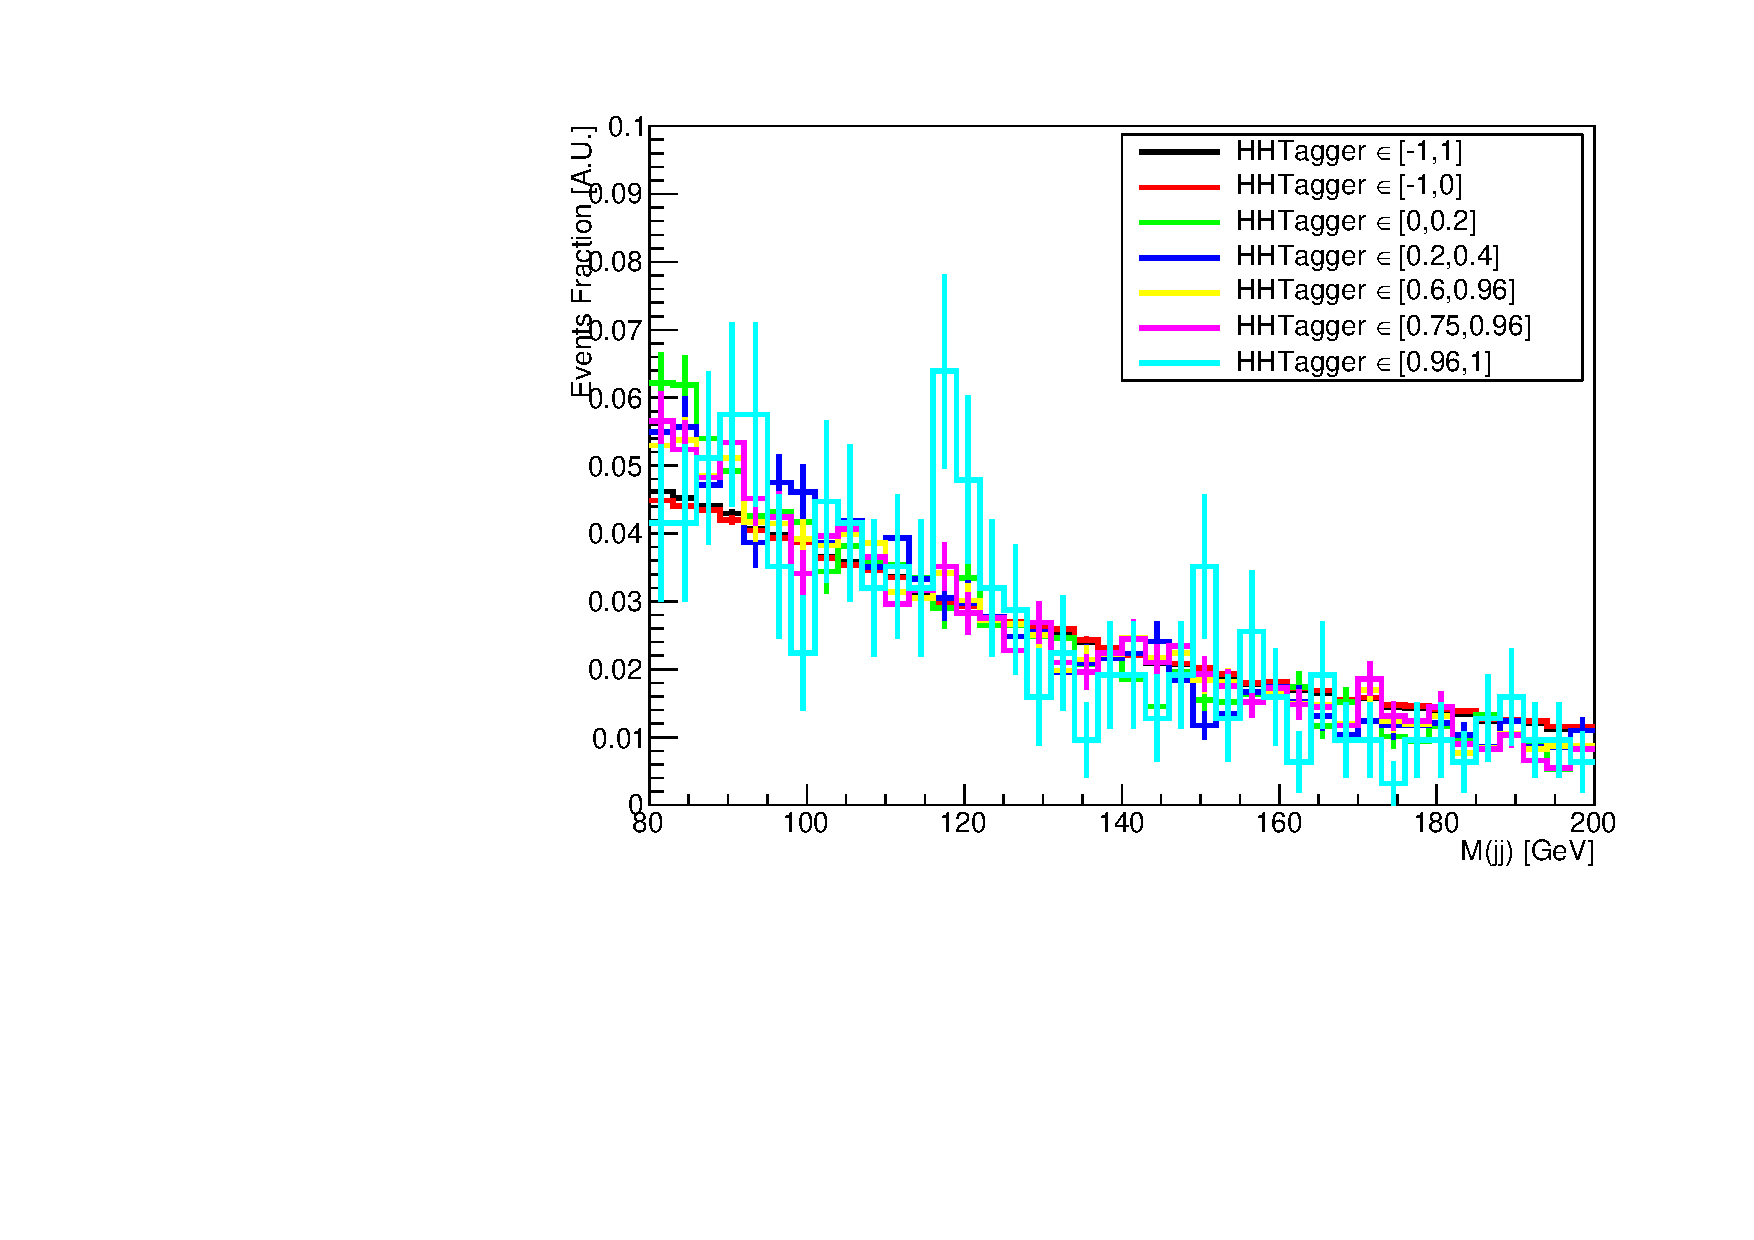
\includegraphics[width=0.45\textwidth]{figures/sec-cats/mva/hhtag_mjj}\hfil
  \caption{$\Mgg$ and $\Mjj$ in bins of HHTagger. Although the slope changes between bins, this effect does not influence the limit setting.}
  \label{fig:mva_mggmjj}
\end{figure*}

\subsubsection{Performance Cross-Checks}

We have performed several cross checks to look for possible improvements on the categorization MVA. 

\begin{itemize}
\item \textbf{Signal Hypothesis}
\end{itemize}

In the standard training, the sum of all non-resonant samples are used as signal hypothesis. 
However, this might not be the optimal training for the SM HH case. 
To test this, we compare the performance of different trainings assuming the SM HH signal. 
The signal hypotheses tested are:
\begin{itemize}
\item All non-resonant (standard);
\item SM HH;
\item SM HH, with separate training for the high mass and low mass region (similar to standard);
\item SM HH + Benchmark 3 (this benchmark point refers to the node that contains the SM point);
\item SM HH + Benchmark 3, with separate training for the high mass and low mass region (similar to standard).
\end{itemize}
The background hypothesis for this test is the photon control region, in the high mass region. 

The ROC curves from the different trainings are shown in Figure \ref{fig:mva_cc_signal}. 
Since no significant improvement is seen in the high purity region (for background rejection larger than 95\%, a typical value for the chosen WPs), the standard training method is kept in use. 

\begin{figure*}[thb]
  \centering
  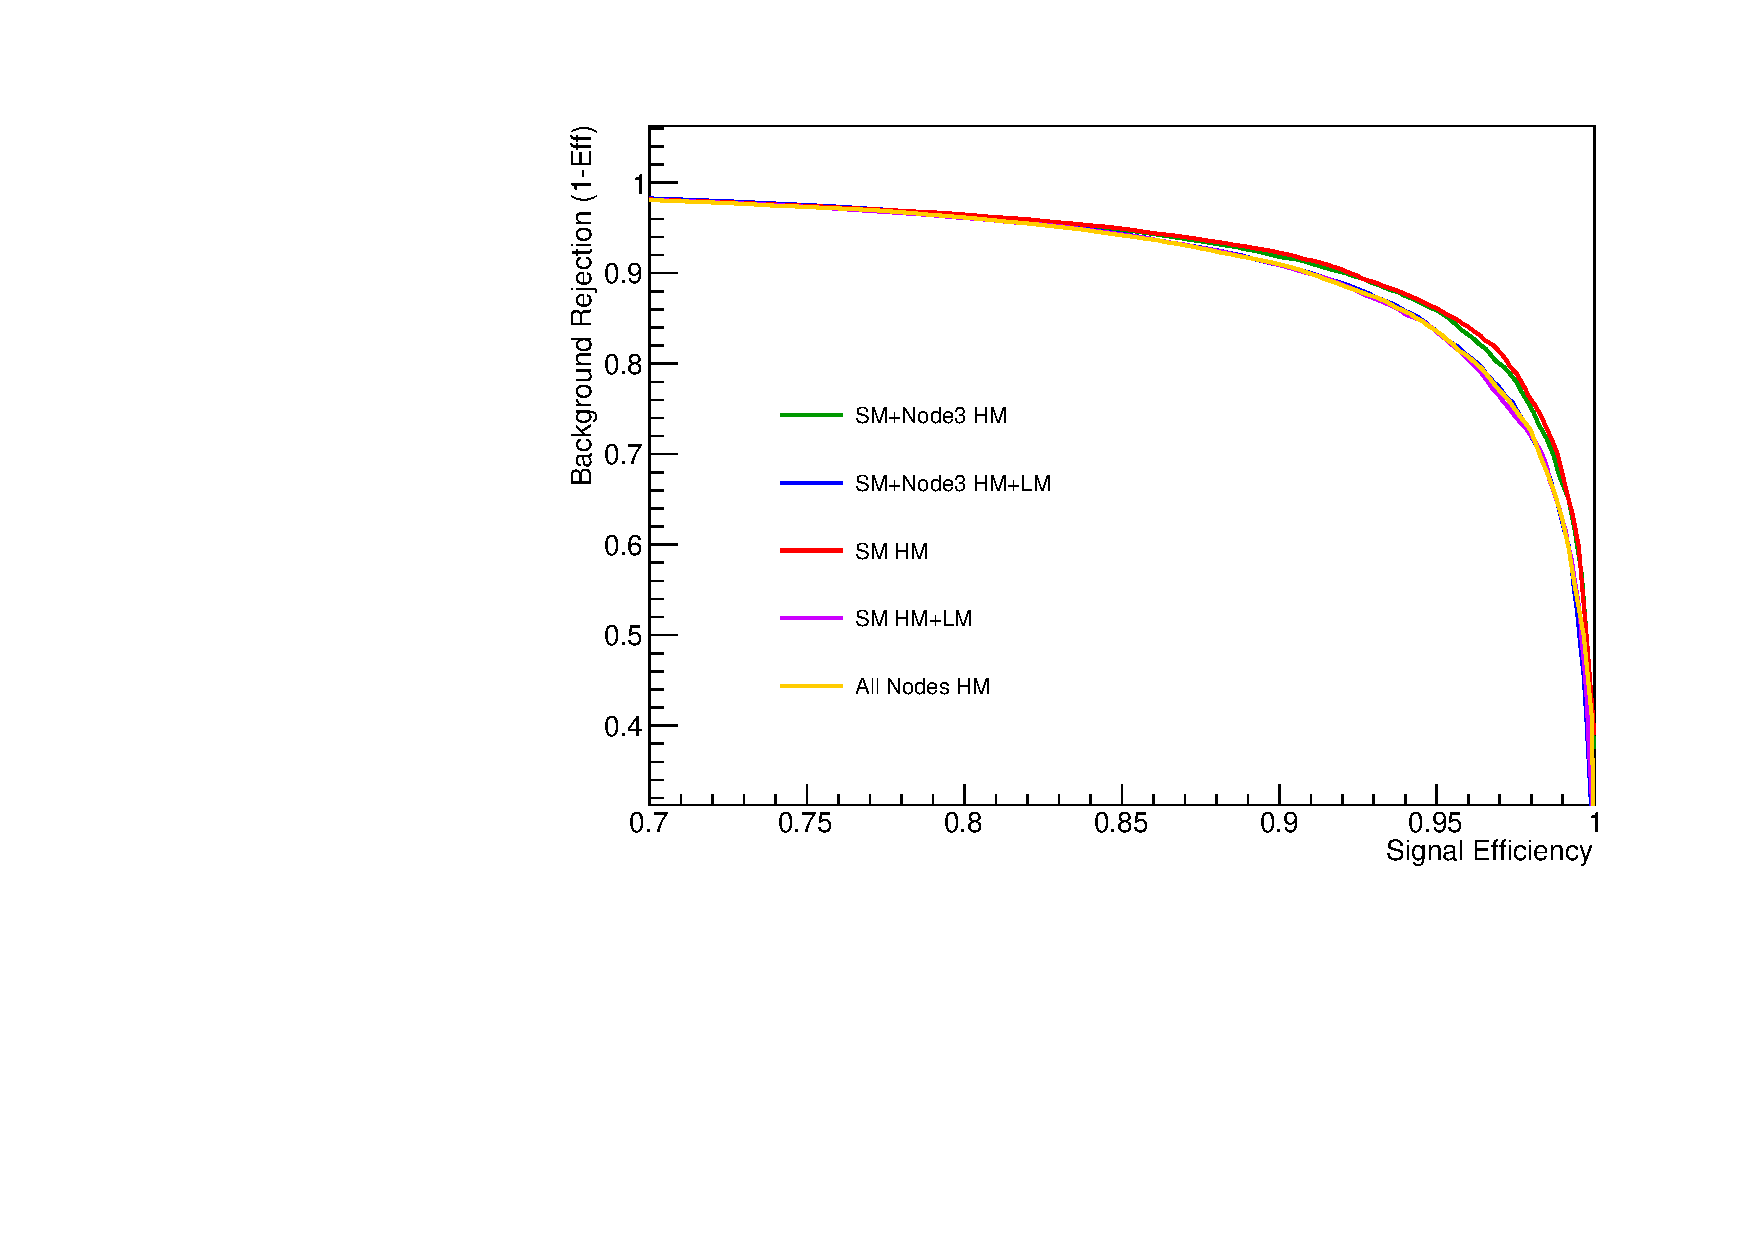
\includegraphics[width=0.7\textwidth]{figures/sec-cats/mva/ROC}\hfil
  \caption{ROC curves with different signal hypotheses for training. The performance is evaluated on the high mass region, with the photon control region as background and SM HH as signal.}
  \label{fig:mva_cc_signal}
\end{figure*}


\begin{itemize}
\item \textbf{Background Hypothesis}
\end{itemize}

In the standard training, the photon control region is used as a background model, avoiding MC reliance. 
However, this might not be the optimal because the photon control region might have different correlation between the MVA variables with respect to the signal region. 
To test this, we compare the performance of different trainings assuming different background hypotheses: 
\begin{itemize}
\item Photon control region (standard);
\item Blinded signal region;
\item Blinded control region (to insure that the difference between the two previous trainings does not come from blinding).
\end{itemize}
The background hypothesis for this test is the blinded signal region, in the high mass region, and the signal hypothesis is SM HH. 

The ROC curves from the different trainings are shown in Figure \ref{fig:mva_cc_background}. 
While some improvement is seen, this training is not optimal for statistical reasons. 
The blinded signal region contains significantly less events than the photon control region. 
This limits the precision and accuracy of the multivariate analysis training. 
Specifically, it has been observed that the blinded signal region does not contain events in the high BDT region (signal-like phase space), which can cause over training. 
The second issue is that, optimally, training on a dataset that is statistically independent from the one to which it will be applied leads to a more robust procedure. 

\begin{figure*}[thb]
  \centering
  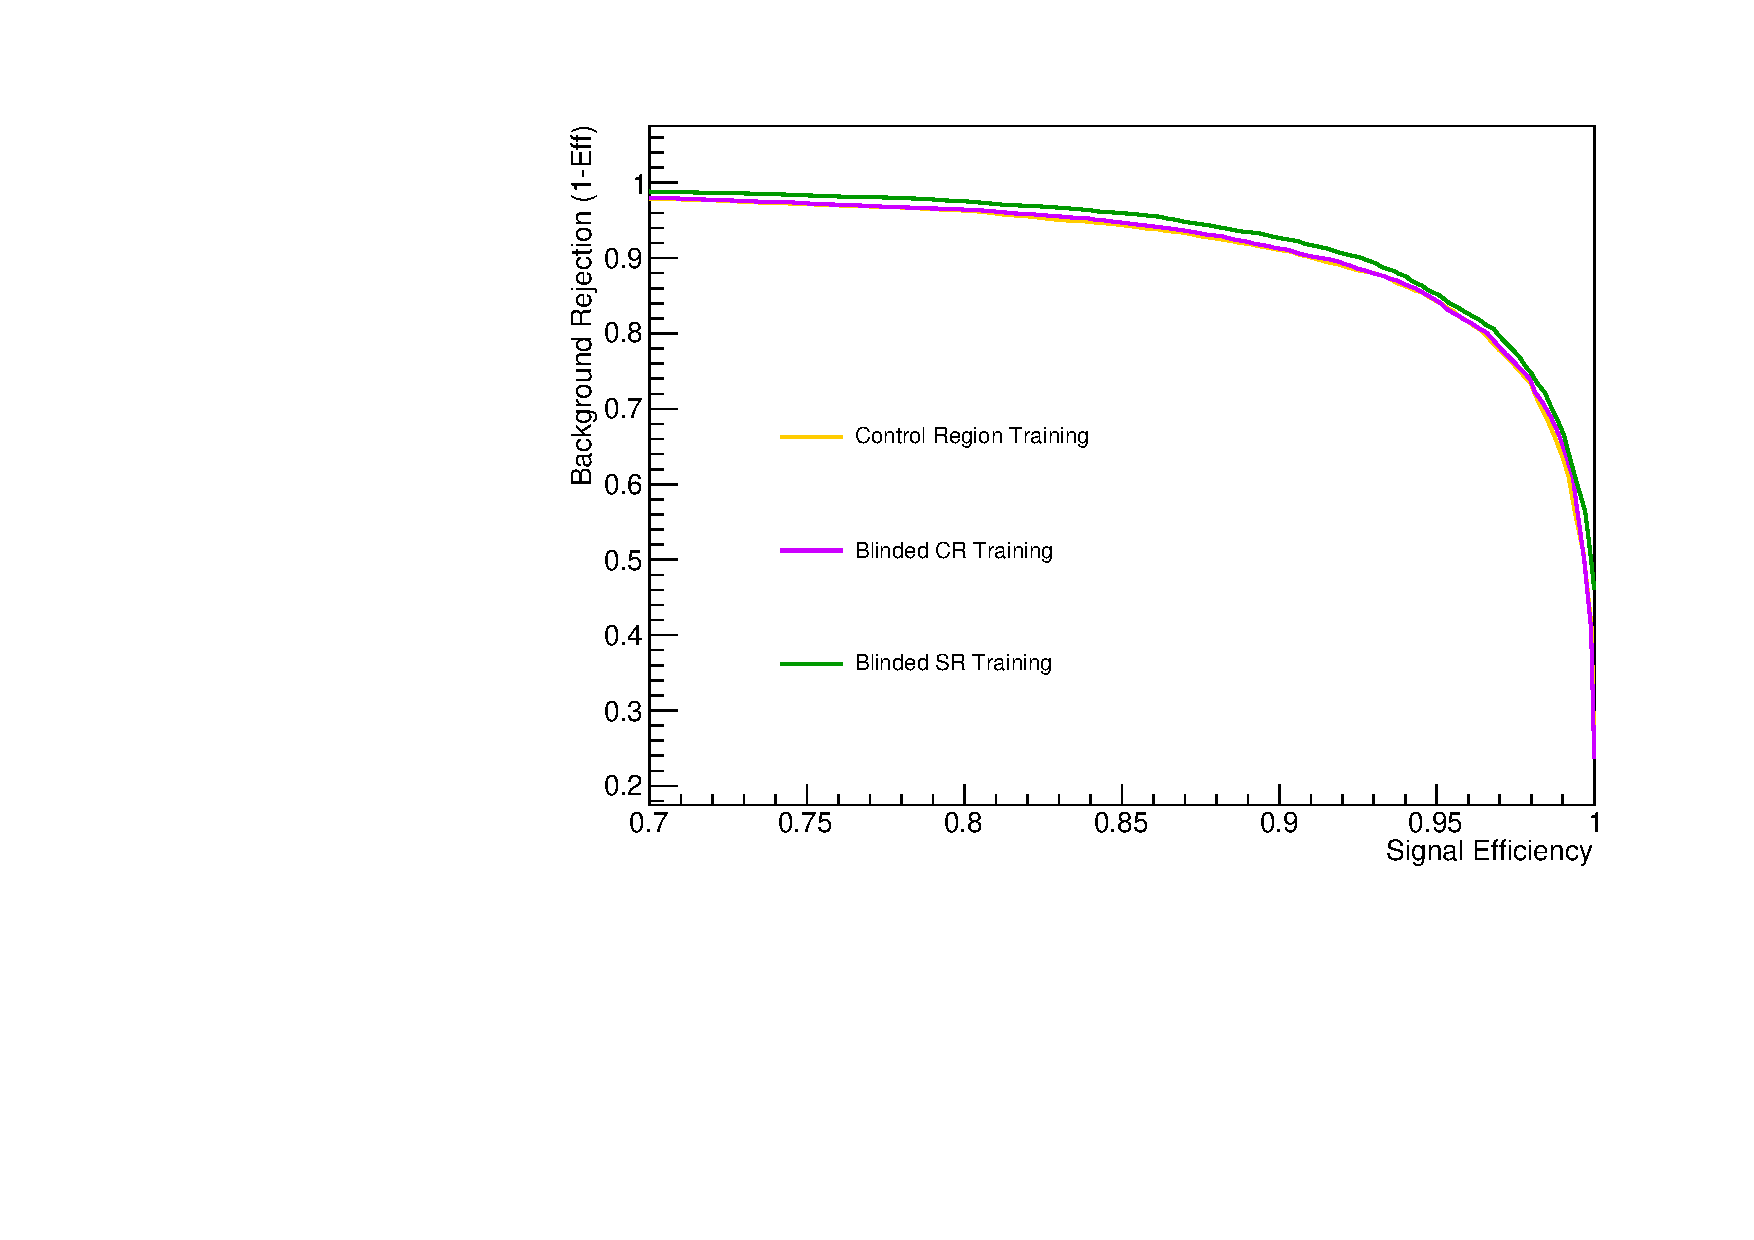
\includegraphics[width=0.7\textwidth]{figures/sec-cats/mva/ROC_BCR}\hfil
  \caption{ROC curves with different background hypotheses for training. The performance is evaluated on the high mass region, with the blinded signal region as background and SM HH as signal.}
  \label{fig:mva_cc_background}
\end{figure*}

\begin{itemize}
\item \textbf{Resonant Hypothesis}
\end{itemize}

While this MVA is trained with the non-resonant signal hypotheses, it can also be applied to the resonant search. 
We check, however, if a dedicated training with the resonant samples as signal hypothesis performs better, when applying the categorization to the resonant analysis.  
This is tested by comparing the categorization performance of the standard training versus a resonant training on a resonant signal point. 
The plot in Figure \ref{fig:mva_cc_res}, these two trainings are shown and no significant difference is seen. 
Therefore the standard, non-resonant training will be used also for the resonant analysis. 

\begin{figure*}[thb]
  \centering
  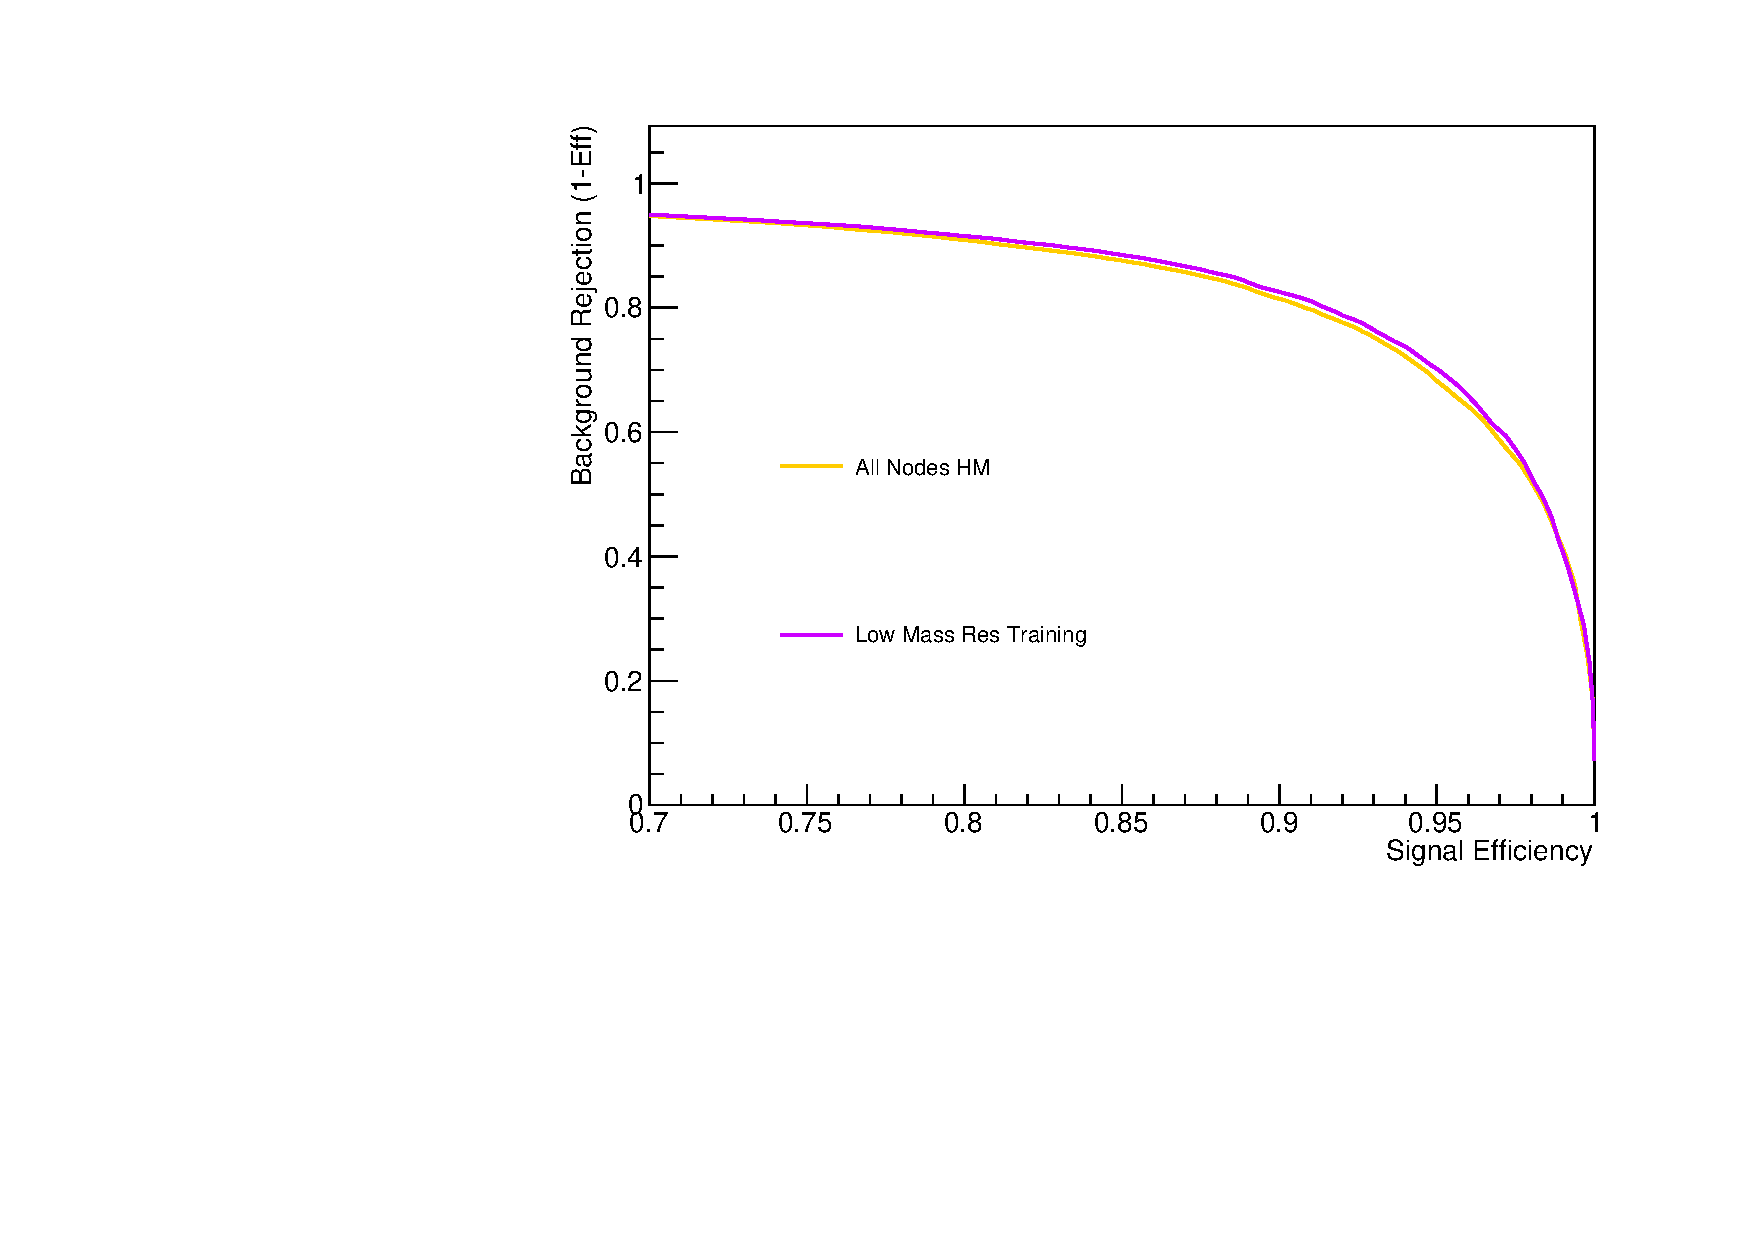
\includegraphics[width=0.7\textwidth]{figures/sec-cats/mva/ROC_res}\hfil
  \caption{ROC curves with different signal hypotheses for training. The performance is evaluated on the high mass region, with the photon control region as background and Radion 300 GeV as signal.}
  \label{fig:mva_cc_res}
\end{figure*}


